\documentclass[12pt twoside]{report}
\usepackage[utf8]{inputenc}
\usepackage{graphicx}
\usepackage{tcolorbox}
\usepackage{hyperref}
\usepackage{geometry}
\usepackage{multicol}
\usepackage{amsmath,tabularx}
\usepackage{subfig}
\usepackage{amsmath}
\usepackage{amssymb}

\newgeometry{
	top=1.5in,
	bottom=1.5in,
	outer=1.5in,
	inner=1.5in
}

\newtheorem{theorem}{Theorem}[section]
\newtheorem{corollary}{Corollary}[theorem]
\newtheorem{lemma}[theorem]{Lemma}

\newtheorem{definition}{Definition}[section]

\title{Notes of Machine Learning}
\author{Anh-Tien Nguyen}

\begin{document}

\maketitle
\chapter*{Abstract}
\tableofcontents

\chapter{Slope and Rates of Changes}

\section{The Slope of a Line}
The content of this section is come from \cite{precalculus}.
\begin{enumerate}
    \item measure the "steepness" of a line
    \item how quickly a line rises (or falls) as we move from left to right
    \item if a line lies in a coordinate plane, then the run is change in the x-coordinate and the rise is the corresponding change in the y-coordinate between any two points on the line.
\end{enumerate}

\begin{theorem}
The slope m of a non-vertical line that passes through the point $A(x_1, y_1)$ and $B(x_2, x_2)$ is 

\begin{equation}
\label{eq:1}
slope = \frac{rise}{run}=\frac{y_2 - y_1}{x_2 - x_1}
\end{equation}

\begin{flushleft}
The slope of a vertical line is not define.
\end{flushleft}

\end{theorem}

\begin{figure}[h]
    \centering
    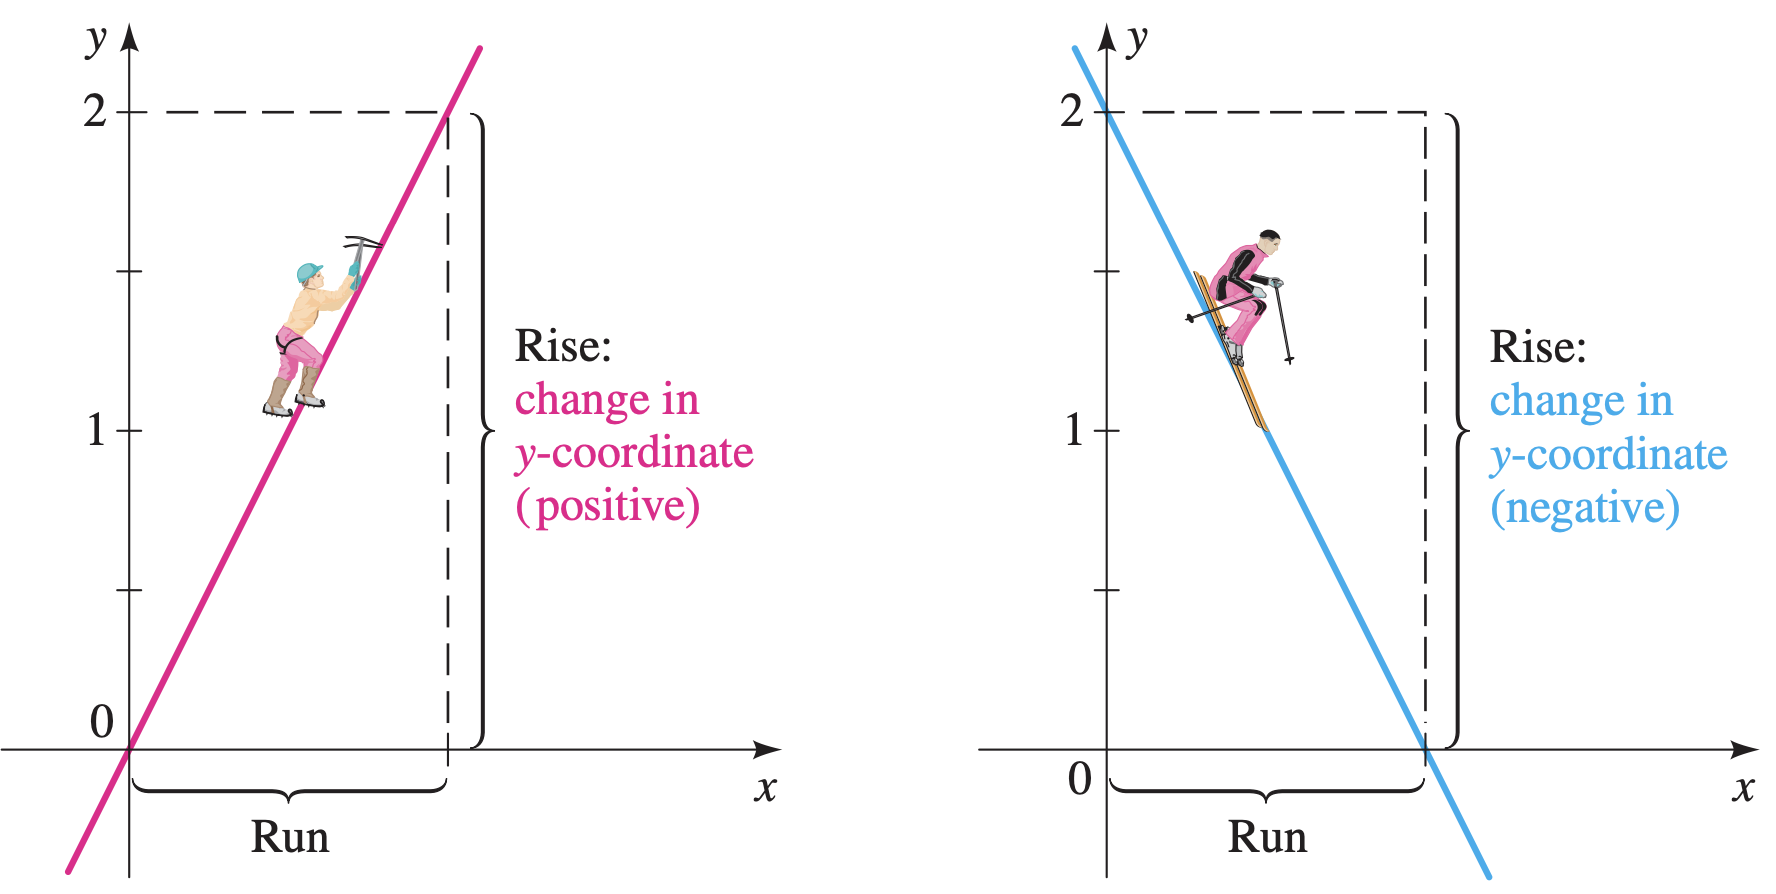
\includegraphics[scale=0.3]{chapter001/figures/fig001}
    \caption{Rise and Run}
    \label{fig:Fig1}
\end{figure}

\newtcolorbox{mybox}[1]{colback=blue!5!white,colframe=blue!75!black,fonttitle=\bfseries,title=#1}
\begin{mybox}{Warning}
The slope is independent of which two points are chosen on the line.
\end{mybox}

\begin{figure}[h]
    \centering
    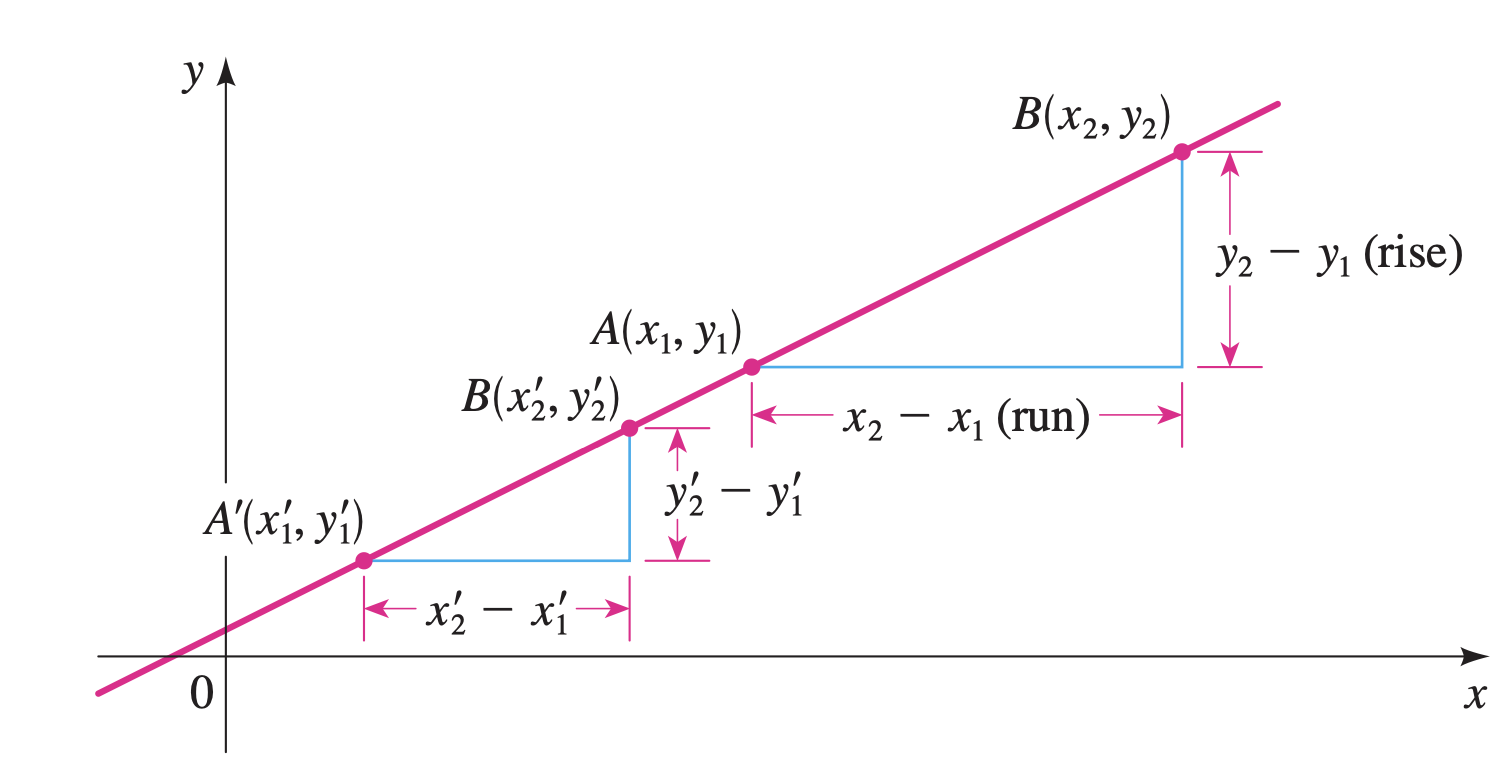
\includegraphics[scale=0.3]{chapter001/figures/fig002}
    \caption{The slope of a vertical line is not define}
    \label{fig:Fig2}
\end{figure}

\begin{figure}[h]
    \centering
    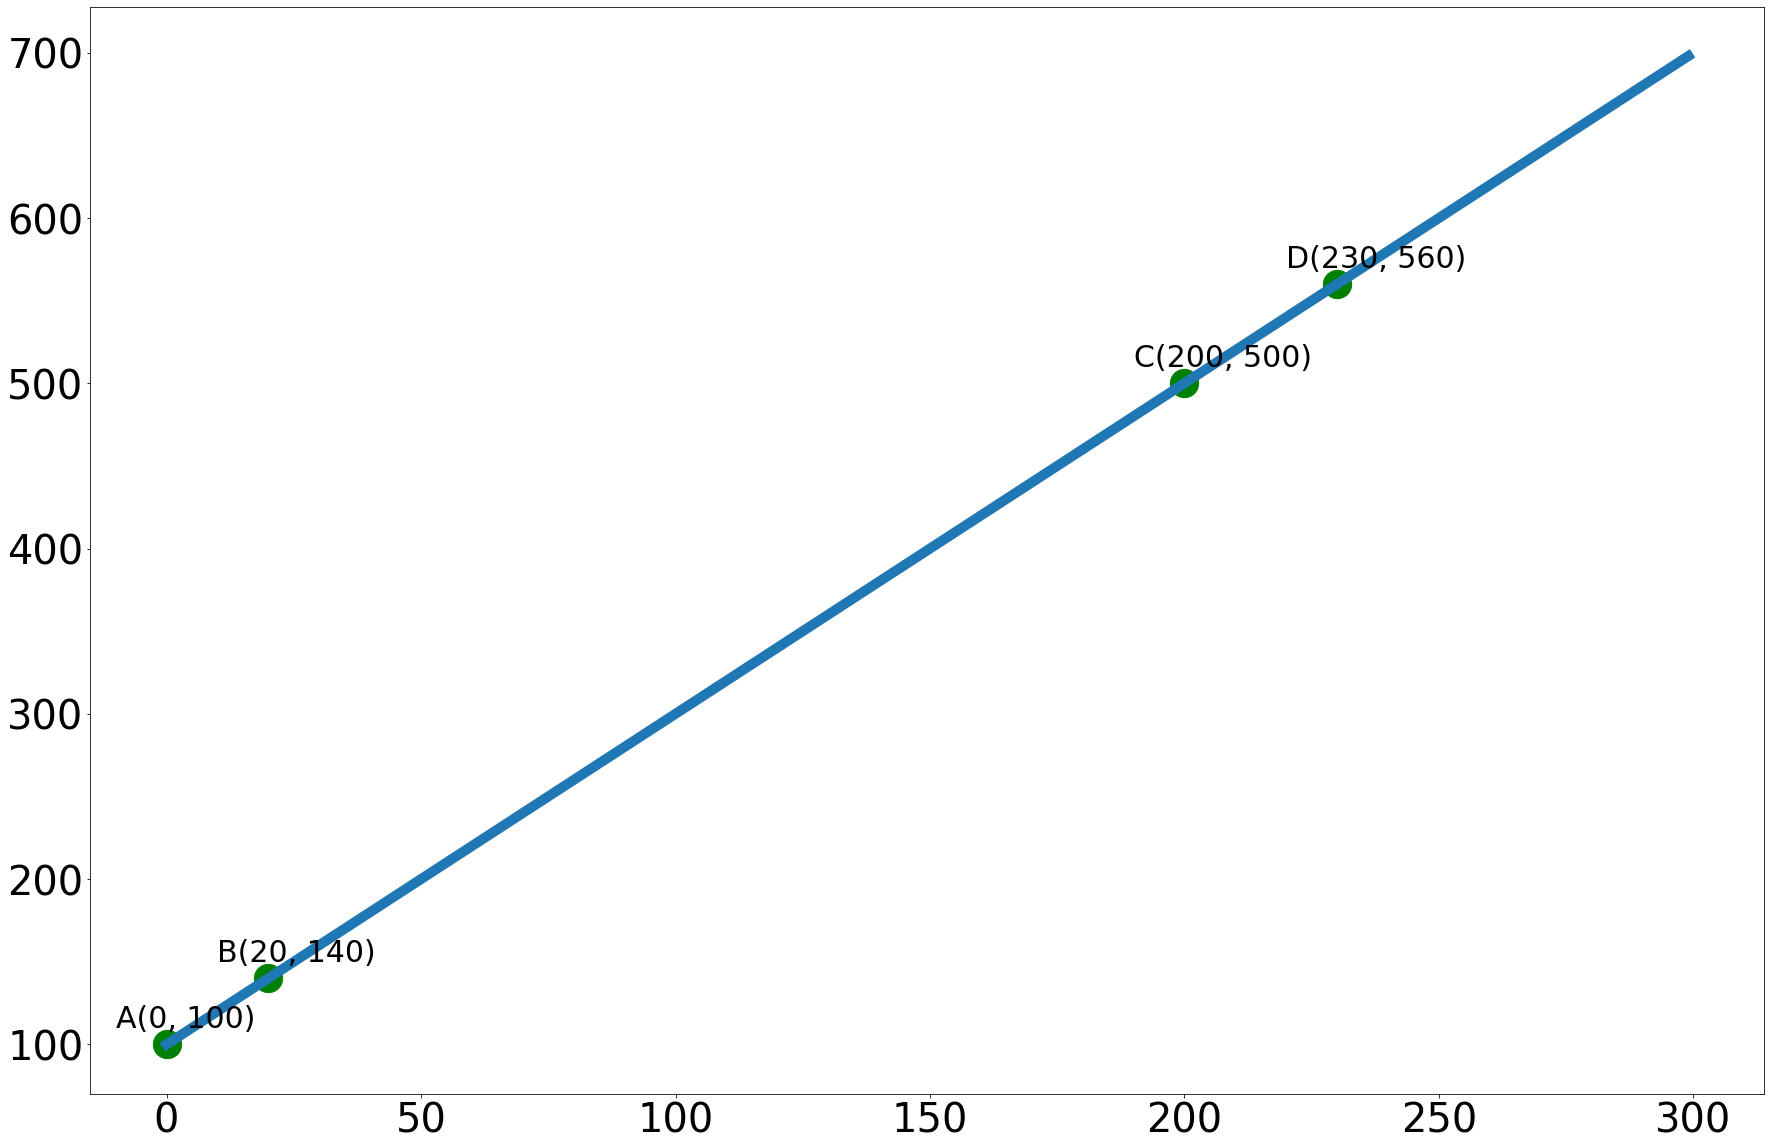
\includegraphics[scale=0.15]{chapter001/figures/fig003}
    \caption{The slope of A and B is the same as C and D}
    \label{fig:Fig3}
\end{figure}

\subsection{Example}
Given 2 lines which are represented by equations $f(x) = 5x + 3$ and $g(x) = 10x + 6$, respectively.

\begin{center}
	\begin{tabular}{ |p{3cm}||p{3cm}|p{3cm}|p{3cm}|}
 		\hline
 		\multicolumn{2}{|c|}{Investigating Steepness Values} \\
 		\hline
 		$f(x) = 5x + 3$ & $g(x) = 10x + 6$\\
 		\hline
 		$x=1, y=8$  & $x=1, y=16$\\
 		$x=2, y=13$ & $x=2, y=26$\\
 		$x=3, y=18$ & $x=3, y=36$\\
 		$x=4, y=23$ & $x=4, y=46$ \\
 		$x=5, y=28$ & $x=5, y=56$\\
 		\hline
	\end{tabular}	
\end{center}

The $g(x)$ is always rise faster than $f(x)$. The steepest lines are those for which the absolute value of the slope is the largest.

\section{Rates of Change} 
\begin{figure}[h]
    \centering
    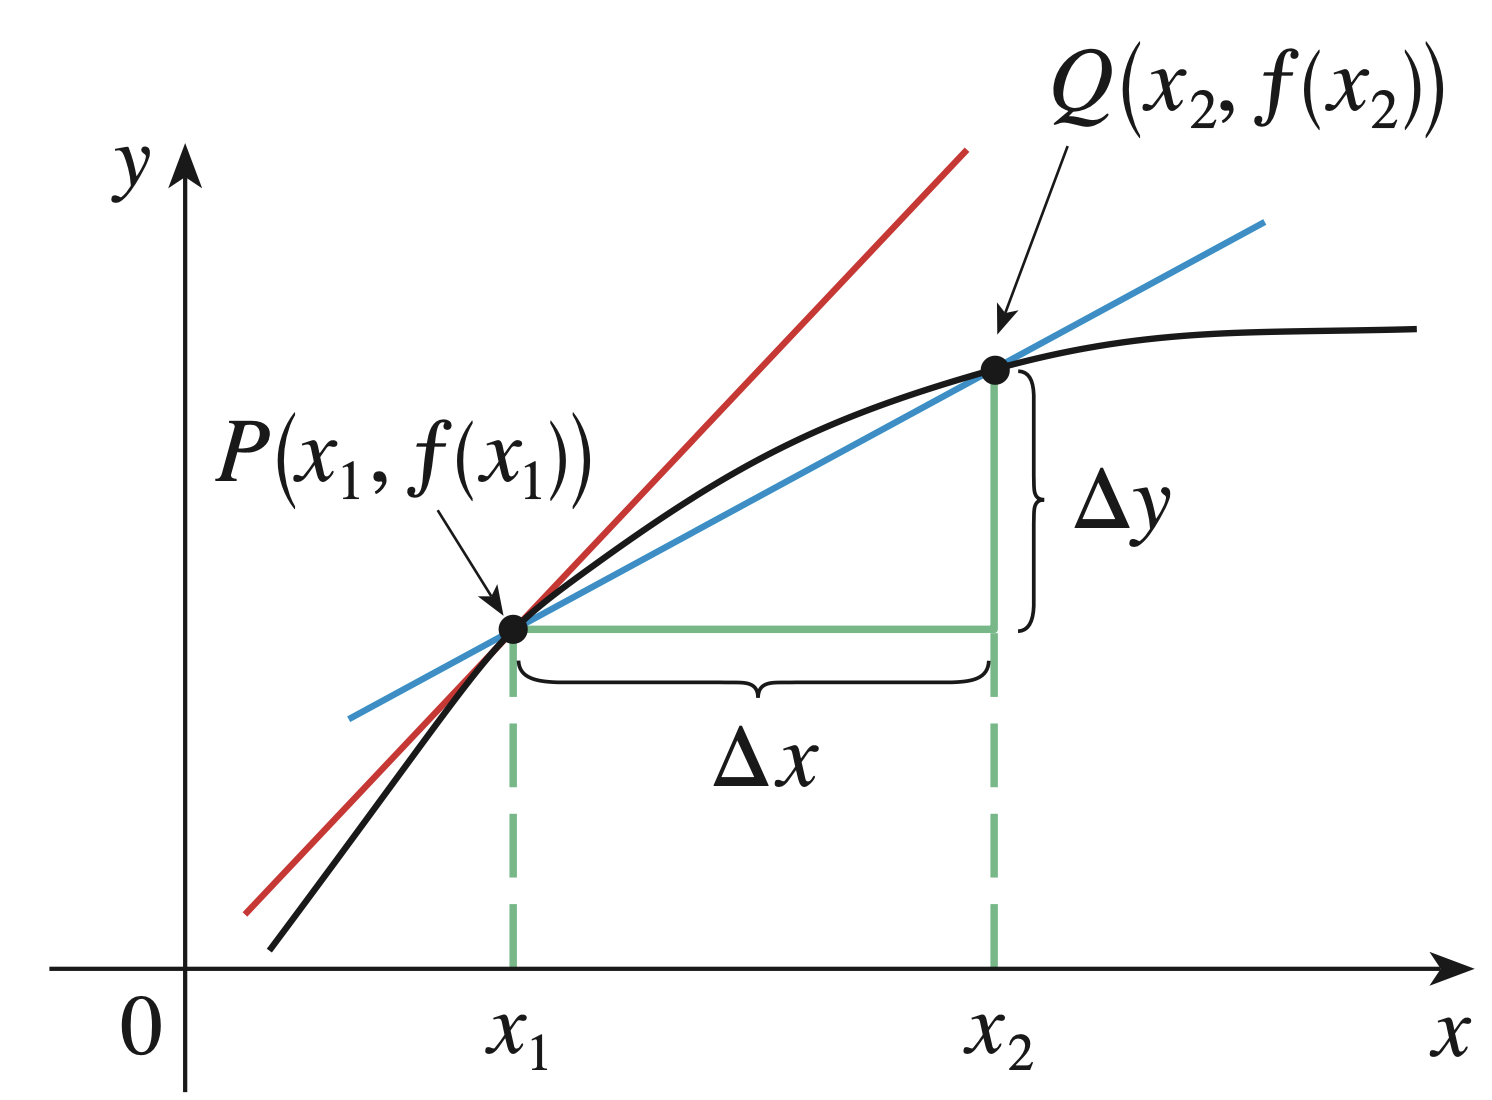
\includegraphics[scale=0.3]{chapter001/figures/fig004}
    \caption{Rates of Change}
    \label{fig:Fig4}
\end{figure}

\begin{flushleft}
\cite{calculus} Given a function $y=f(x)$, if $x$ changes from $x_1$ to $x_2$, then the change in $x$ is $\Delta x = x_2 - x_1$ and the corresponding change in $y$ is $\Delta y = f(x_2) - f(x_1)$.
\end{flushleft}

\begin{flushleft}
The difference quotient

\begin{equation}
\label{eq:2}
\frac{\Delta y}{\Delta x} = \frac{f(x_2) - f(x_1)}{x_2 - x_1}
\end{equation}

is called the \textbf{average rate of change of y with respect to x} over the interval $[x_1, x_2]$ and can be interpreted as the slope of the secant line $PQ$ in Figure \ref{fig:Fig4}

We now consider the average rate of change over smaller and smaller intervals by letting $x_2$ approach $x_1$ and therefore letting $\Delta x$ approach 0.

The limit of these average rates of change is called the (\textbf{instantaneous}) \textbf{rate of change of $y$ with respect to $x$} at $x = x_1$, which is interpreted as the slope of the tangent to the curve $y = f(x)$ at $P(x_1, f(x_1))$
\end{flushleft}

\begin{equation}
\label{eq:3}
instantaneous\ rate\ of\ change = \lim_{\Delta x \to 0} \frac{\Delta y}{\Delta x} = \lim_{x_2 \to x_1} \frac{f(x_2) - f(x_1)}{x_2 - x_1}
\end{equation}

\begin{flushleft}
We recognize this limit as being the derivative $f'(x_1)$.
we know the one interpretation of the derivative $f'(a)$ is as the slope of the tangent line to the curve $y=f(x)$ when $x=a$
\end{flushleft}

\begin{mybox}{Derivative}
The derivative $f'(a)$ is the instantaneous rate of change of $y=f(x)$ with respect to $x$ when $x = a$.
\end{mybox}

\begin{flushleft}
The connection with the first interpretation is that if we sketch the curve $y = f(x)$, then the instantaneous rate of change is the slope of the tangent to this curve at the point where $x = a$.

This means that when the derivative is large, the y-values change rapidly. When the derivative is small, the curve is relatively flat (as at point $Q$) and the y-values changes slowly.
\end{flushleft}

\section{Partial Derivative}
\begin{definition}
If $f$ is a function of two variables, its partial derivatives are the functions $f_x$ and $f_y$ defined by
\end{definition}
\begin{equation}
    \label{eq:7}
    f_x(x, y) = \lim_{\Delta h \to 0} \frac{f(x+h, y)-f(x, y)}{h}
    f_y(x, y) = \lim_{\Delta h \to 0} \frac{f(x, y + h)-f(x, y)}{h}
\end{equation}

\subsection{Example}
If $f(x, y)=x^3+x^2y^3-2y^2$, find $f_x(2,1)$ and $f_y(2,1)$.
\subsubsection{Solution}
$$
    f_x(x, y) = 3x^2 + 2xy^3
$$
and
$$
    f_x(x, y) = 3x^2y^2 - 4y
$$
therefore,
$$
    f_x(2, 1) = 12 + 4 = 16
$$
$$
    f_y(2, 1) = 12 - 4 = 8
$$

\section{Interpretations of Partial Derivatives}

Given an equation $z=f(x, y)$ which represents a surface $S$ (the graph of $f$). If $f(a, b)=c$, then the point $P(a, b, c)$ lies on $S$. As described in the Figure \ref{fig:Fig7}, by fixing $y=b$, we are restricting our attention to the curve $C_1$ in which the vertical plane $y=b$ intersects S. Likewise, the vertical plane $x=a$ intersect $S$ in a curve $C_2$. Both of the curves $C_1$ and $C_2$ pass through the Point $P$.

Note that the curve $C_1$ is the graph of the function $g(x)=f(x, b)$, so the slope of its tangent $T_1$ at $P$ is $g'(a)=f_x(a, b)$. The curve $C_2$ is the graph of the function $G(y)=f(a, y)$, so the slope of its tangent $T_2$ at $P$ is $G'(b)=f_y(a, b)$.

Thus the partial derivatives $f_x(a, b)$ and $f_y(a, b)$ can be interpreted geometrically as the slope of the tangent lines at $P(a, b, c)$ to the traces $C_1$ and $C_2$ of $S$ in the plane $y=b$ and $x=a$.

\subsection{Example}

\cite{calculus} The body mass index (BMI) of a person as

\begin{equation}
    \label{eq:8}
    B(m, h)=\frac{m}{h^2}
\end{equation}

Calculate the partial derivatives of $B$ for a young man with $m=64kg$ and $h=1.68m$ and interpret them.

\subsubsection{Solution}

$$
    \frac{\partial B}{\partial m}(m, h)=\frac{\partial}{\partial m}(\frac{m}{h^2})=\frac{1}{h^2}
$$
so
$$
    \frac{\partial B}{\partial m}(64, 1.68)=\frac{1}{(1.68)^2} \approx 0.35(kg/m^2)/kg
$$
This is the rate at which the man's BMI increases with respect to his weight when he weights $64kg$ and his height is $1.68m$. So if this weight increases by a small amount, one kilogram for instance, and his height remains unchanged, then his BMI will increase from $B(64, 1.68) \approx 22.68$ by about 0.35.

Now we regard $m$ as a constant. The partial derivative with respect to $h$ is 

$$
    \frac{\partial B}{\partial h}(m, h) = \frac{\partial }{\partial h}(\frac{m}{h^2})=m(-\frac{2}{h^3}) = -\frac{2m}{h^3}
$$
so
$$
    \frac{B}{h}(64, 1.68)=-\frac{2 \cdot 64}{(1.68)^3} \approx -27(kg/m^2)/m
$$
This is the rate at which the man's BMI increases with respect to his height when he weights $64kg$ and his height is $1.68m$. If the man is still growing and his weight stays unchanged while his height \textbf{increases} by a small amount, say 1 cm, then his BMI will \textbf{decrease} by about $27(0.01) = 0.27$.


\begin{figure}[h]
    \centering
    \cite{calculus}
    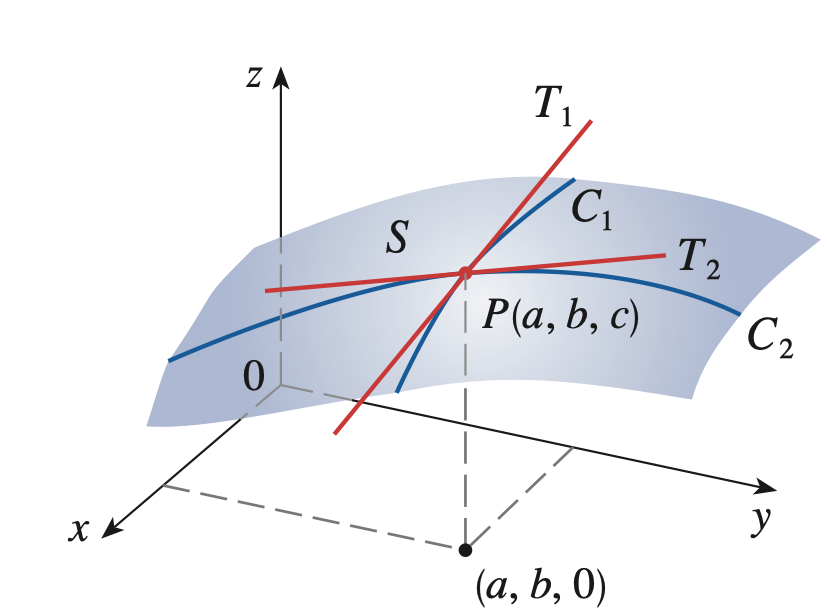
\includegraphics[scale=0.6]{chapter001/figures/fig007}
    \caption{The partial derivatives of $f$ at $(a, b)$ are the slope of the tangents to $C_1$ and $C_2$}
    \label{fig:Fig7}
\end{figure}

\section{The Chain Rule}

\begin{definition}
If $g$ is differentiable at $x$ and $f$ is differentiable at $g(x)$, then the composite function $F=f \circ g$ defined by $F(x)=f(g(x))$ is differentiable at $x$ and $F'$ is given by the product
    \begin{equation}
	   \label{eq:9}
	   F'(x) = f'(g(x)) \cdot g'(x)
    \end{equation}
In Leibniz notation, if $y=f(u)$ and $u=g(x)$ are both differentiable functions, then
    \begin{equation}
	   \label{eq:10}
	   \frac{dy}{dx}=\frac{dy}{du}\frac{du}{dx}
    \end{equation}
\end{definition}

\subsection{Example}

\cite{calculus}, page 202. Differentiate (a) $y=sin(x^2)$ and (b) $y=sin^2x$.

\subsubsection{Solution}
(a) If $y=sin(x^2)$, then the outer function is the sine function and the inner function is the squaring function, so the Chain Rule gives
$$
    \frac{dy}{dx}=\frac{d}{dx}sin(x^2)=2x \cdot cos(x^2)
$$
(b) Note that $sin^2x=(sinx)^2$,
$$
    \frac{dy}{dx}=\frac{d}{dx}(sinx)^2=2 \cdot sinx \cdot cosx
$$

\begin{definition}
Suppose that $z=f(x, y)$ is a differentiable function of $x$ and $y$, where $x=g(t)$ and $y=h(t)$ are both differentiable functions of t. Then z is a differentiable function of $t$ and

    \begin{equation}
        \label{Chain Rule Case 1}
        \frac{dz}{dt}=\frac{\partial f}{\partial x}\frac{\partial x}{\partial t} + \frac{\partial f}{\partial y}\frac{\partial y}{\partial t}
    \end{equation}
\end{definition}

\begin{definition}
    Suppose that $z=f(x, y)$ is a differentiable function of $x$ and $y$, where $x=g(s, t)$ and $y=h(s, t)$ are differentiable functions of $s$ and $t$.
\end{definition}
\noindent
\begin{tabularx}{\linewidth}{@{}XX@{}}
    \begin{equation}
        \label{Chain Rule Case 2}
        \frac{dz}{dt}=\frac{\partial z}{\partial x}\frac{\partial x}{\partial t} + \frac{\partial z}{\partial y}\frac{\partial y}{\partial t}
    \end{equation}
    &
    \begin{equation}
        \label{Chain Rule Case 2}
        \frac{dz}{ds}=\frac{\partial z}{\partial x}\frac{\partial x}{\partial s} + \frac{\partial z}{\partial y}\frac{\partial y}{\partial s}
    \end{equation}
\end{tabularx}

\begin{definition}
    Suppose that $u$ is a differentiable function of the $n$ variables $x_1, x_2, ..., x_n$ and each $x_j$ is a differentiable function of the $m$ variables $t_1, t_2, ..., t_m$. Then $u$ is a function of $t_1, t_2, ..., t_m$ and
    \begin{equation}
        \label{The General Chain Rule}
        \frac{\partial u}{\partial t_i} = \frac{\partial u}{\partial x_1}\frac{\partial x_1}{\partial t_i} + \frac{\partial u}{\partial x_2}\frac{\partial x_2}{\partial t_i} + ...+ \frac{\partial u}{\partial x_n}\frac{\partial x_n}{\partial t_i}
    \end{equation}
    for each $i=1, 2, ..., m$.
\end{definition}

\subsection{Example}
The pressure $P$ (in kilopascals), volume $V$ (in liters), and temperature $T$ (in kelvins) of a mole of an ideal gas are related by equation $PV=8.31T$. Find the rate at which the pressure is changing when the temperature is $300K$ and increasing at a rate of $0.1K/s$ and the volume is $100L$ and increasing at a rate of $0.2L/s$. (Finding the rate change of $P$)(\cite{calculus}, page 1024)

\subsubsection{Solution}
If $t$ represents the time elapsed in seconds, then at the given instant we have $T=300$, $\frac{dT}{dt}=0.1$, $V=100$, $\frac{dV}{dt}=0.2$. Since
$$
    P = 8.31\frac{T}{V}
$$
thus,
$$
    \Rightarrow \frac{\partial P}{\partial T} = \frac{8.31}{V}
$$
and
$$
    \Rightarrow \frac{\partial P}{\partial V}=-\frac{8.31T}{V^2}
$$
Therefore,
\begin{equation}
    \frac{\partial P}{\partial t}=\frac{\partial P}{\partial T}\frac{\partial T}{\partial t} + \frac{\partial P}{\partial V}\frac{\partial V}{\partial t}=\frac{8.31}{V}\frac{\partial T}{\partial t} - \frac{8.31 T}{V^2}\frac{\partial V}{\partial t}=\frac{8.31}{100}(0.1)-\frac{8.31(300)}{100^2}(0.2)=-0.04155
\end{equation}
The pressure is decreasing at a rate of about $0.042 kPa/s$.

\subsection{Example}
If $z=e^x \sin y$, where $x=st^2$ and $y=s^2t$, find $\partial z / \partial s$ and $\partial z / \partial t$.
\subsubsection{Solution}
$$
    \frac{\partial z}{\partial s}=\frac{\partial z}{\partial x}\frac{\partial x}{\partial s} + \frac{\partial z}{\partial y}\frac{\partial y}{\partial s} = (e^x \sin y)(t^2) + (e^x \cos y)(2st)
$$
$$
    \frac{\partial z}{\partial t}=\frac{\partial z}{\partial x}\frac{\partial x}{\partial t} + \frac{\partial z}{\partial y}\frac{\partial y}{\partial t} = (e^x \sin y)(2st) + (e^x \cos y)(s^2)
$$

\section{Derivatives of General Exponential Functions}
This content is recommended by \cite{calculus}, page 204.
\begin{theorem}
\begin{equation}
    \label{eq:11}
    \frac{d}{dx}(b^x)=b^x\ln b
\end{equation}    
\end{theorem}

\begin{theorem}
If $n$ is any real number and $u=g(x)$ is differentiable, then
\begin{equation}
    \label{eq:12}
     \frac{d}{dx}(u^n)=nu^{n-1}\frac{du}{dx}
\end{equation}
Alternatively,
\begin{equation}
    \label{eq:12}
     \frac{d}{dx}[(g(x)]^n=n[(g(x)]^{n-1} \cdot g'(x)
\end{equation}    
\end{theorem}

\subsection{Example}
Differentiate $y=(x^3 - 1)^{100}$
\subsubsection{Solution}
Taking $u=g(x)=x^3 - 1$ and $n=100$, we have
$$
    \frac{dx}{dy}=\frac{d}{dx}(x^3 - 1)^{100}=100(x^3 - 1)^{99}\frac{d}{dx}(x^3 - 1)=100(x^3-1)^{99} \cdot 3x^2=300 x^2(x^3-1)^{99}
$$

\subsection{Example}
Differentiate $h(x)=5^{x^2}$

\subsubsection{Solution}
$$
    \frac{dh}{dx}=\frac{d}{dx}(5^{x^2})=5^{x^2} \ln 5 \cdot \frac{d}{dx}(x^2)=2x \cdot 5^{x^2} \ln 5 
$$

\section{Applications in Medicine}

\subsection{Measuring the Rate of Increase of Blood Alcohol Concentration}

Biomedical scientists have studied the chemical and physiological changes in the body that result from alcohol consumption. The reaction in the human body occurs in two stages: a fairly rapid process of absorption and a more gradual one of metabolism. Biomedical scientists have studied the chemical and physiological changes in the body that result from alcohol consumption. The reaction in the human body occurs in two stages: a fairly rapid process of absorption and a more gradual one of metabolism.

Medical researchers measured the blood alcohol concentration (BAC) of eight fasting adult male subjects after rapid consumption of $15 mL$ of ethanol (corresponding to one alcoholic drink).1 The data they obtained were modeled by the concentration function. The graph of C is shown in Figure \ref{fig:Fig5}

\begin{equation}
\label{eq:4}
C(t) = 0.0225te^{-0.0467t}
\end{equation}

where $t$ is measured in minutes after consumption and $C$ is measured in $mg/mL$. How quickly is the BAC increasing after 10 minutes?

\begin{figure}[h]
    \centering
    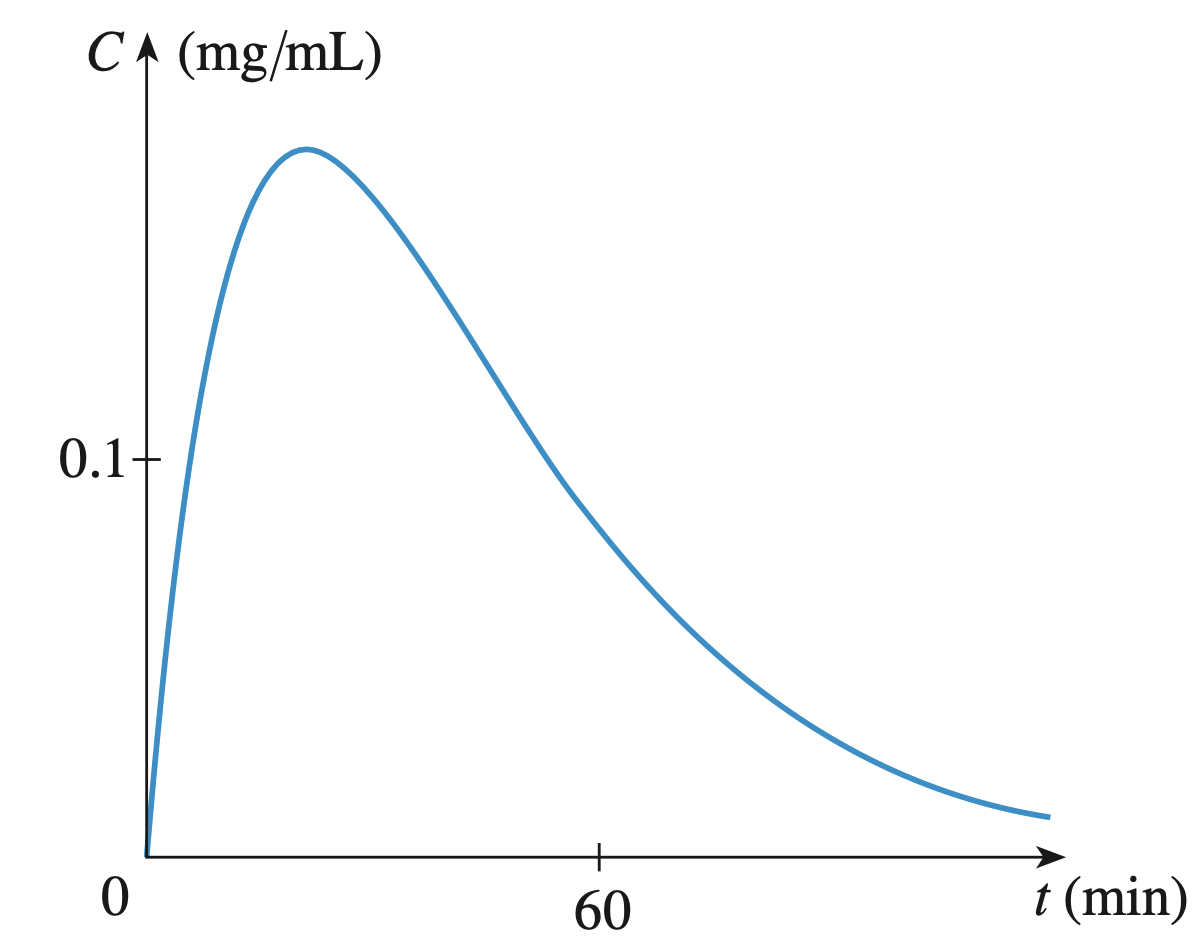
\includegraphics[scale=0.3]{chapter001/figures/fig005}
    \caption{Blood Alcohol Concentration}
    \label{fig:Fig5}
\end{figure}

\begin{center}
	\begin{tabular}{ |p{3cm}||p{3cm}|p{3cm}|p{3cm}|}
 		\hline
 		\multicolumn{2}{|c|}{Investigating Steepness Values} \\
		\hline
 		Time interval & Average rate of change\\
		\hline
 		$10 \leq t \leq 11$    & 0.00703\\
 		$10 \leq t \leq 10.5$  & 0.00727\\
 		$10 \leq t \leq 10.1$  & 0.00747\\
 		$10 \leq t \leq 10.01$ & 0.00751 \\
 		$9 \leq t \leq 10$     & 0.00804\\
 		$9.5 \leq t \leq 10$   & 0.00777\\
 		$9.9 \leq t \leq 10$   & 0.00757\\
 		$9.99 \leq t \leq 10$  & 0.00752\\
 		\hline
	\end{tabular}
\end{center}


\begin{flushleft}
It appears that as we shorten the time period, the average rate of change is becoming closer and closer to a number between 0.00752 and 0.00753 (mg/mL)/min. The instantaneous rate of change at t = 10 is defined to be the limiting value of these average rates of change over shorter and shorter time periods that start or end at t = 10. So we estimate that the BAC increased at a rate of about 0.0075 (mg/mL)/min.

we estimated that the rate of increase of the blood alcohol concentration when $t = 10$ is about 0.0075 (mg/mL)/min. The equation of the curve is \ref{eq:4} which gives $C(10) \approx 0.14105$. So, using the point-slope equation of a line, we get that an approximate equation of the tangent line at $t=10$ is 
\end{flushleft}

\begin{equation}
\label{eq:5}
C - 0.14105 = 0.0075(t - 10)
\Leftrightarrow C = 0.06605 + 0.0075t
\end{equation}

\subsection{Malarial parasites}
The following table, supplied by Andrew Read, shows experimental data involving malarial parasites. The time t is measured in days and N is the number of parasites per micro-liter of blood.

\begin{center}
	\begin{tabular}{ |p{3cm}||p{3cm}|p{3cm}|p{3cm}|}
 		\hline
 		\multicolumn{2}{|c|}{Investigating Steepness Values} \\
 		\hline
 		t & N\\
 		\hline
 		1    & 228\\
 		2    & 2,357\\
 		3    & 12,750\\
 		4    & 26,661\\
 		5    & 372,331\\
 		6    & 2,217,441\\
 		\hline
	\end{tabular}	
\end{center}


\begin{flushleft}
(a) Find the average rates of change of N with respect to t over the intervals [1, 3], [2, 3], [3, 4], and [3, 5].\\
(b) Interpret and estimate the value of the derivative N'(3).
\end{flushleft}

\subsubsection{Solution}

\begin{flushleft}
(a) The average rate of change over [1, 3] is
$$\frac{N(3) - N(1)}{3 - 1} = \frac{12,750 - 228}{2} = 6261 (parasites/\mu L)/day$$
Similar calculations give the average rates of change in the following table:
\end{flushleft}

\begin{center}
	\begin{tabular}{ |p{3cm}||p{3cm}|p{3cm}|p{3cm}|}
 		\hline
 		\multicolumn{2}{|c|}{Investigating Steepness Values} \\
 		\hline
 		Interval & Rate of change\\
 		\hline
 		$[1, 3]$ & 6,261\\
 		$[2, 3]$ & 10,393\\
 		$[3, 4]$ & 13,911\\
 		$[3, 5]$ & 179,791\\
 		\hline
	\end{tabular}	
\end{center}

\begin{flushleft}
(b) The derivative $N'(3)$ means the rate of change of N with respect to $t$ when $t=3$ days.
	$$
		N'(3) = \lim_{\Delta t \to 3} \frac{N(t) - N(3)}{t - 3}
	$$
\end{flushleft}

\subsection{\href{https://www.slideshare.net/ichazalia/derivative-application-in-medical-and-biology}{Growth Rate of Tumor}}

\begin{flushleft}
This example is recommended by \cite{azalia}.\\
There are 3 certain levels of a tumor regarding to its malignancy.
\begin{enumerate}
    \item The first level is benign tumor. It does not invade nearby or spread to other parts of the body.
    \item The second level is premalignant or precancerous tumor which is not yet malignant, but is about to become so.
    \item The last level is malignant tumors. These are cancerous tumors, they tend to become progressively worse, and can potentially result in death.
\end{enumerate}

The rate at which a tumor grows is directly proportional to its volume. Larger tumors grow faster and smaller tumors grow slower.
The volume of a tumor is found by using the exponential growth model which is
	$$
		V(t) = V_0 \cdot e^{kt}
	$$
	where
	
\begin{enumerate}
    \item $V_0$ = initial volume.
    \item e     = exponential growth (2.7182...)
    \item k     = growth constant
    \item t     = time
\end{enumerate}

(a) Find the rate of change of a tumor when its initial volume is $10cm^3$ with a growth constant of 0.075 over a time period of 7 years.\bigbreak
(b) Find the rate of change of a tumor when its initial volume is $2cm^3$ with a growth constant of 0.075 over a time period of 7 years.
\end{flushleft}

\subsubsection{Solution}

The rate of change of a tumor is the derivative of $V(t)$ with respect to $t$
$$
	\frac{\partial v}{\partial t}=\frac{\partial (V_0 \cdot e^{kt})}{\partial t} = k \cdot (V_0 \cdot e^{kt}) = k \cdot (V(t))
$$

(a) 
$$
V(7) = 10 \cdot e^{0.075 \cdot 7} = 16.905(cm^3)
$$
$$
V'(7) = 0.075 \cdot V(7) = 1.267875(cm^3)/year
$$

(b)
$$
V(7) = 2 \cdot e^{0.075 \cdot 7} = 3.3809(cm^3)
$$
$$
V'(7) = 0.075 \cdot V(7) = 0.2535675(cm^3)/year
$$

\begin{mybox}{Question}
What is the tumor growth constant $k$?
\end{mybox}

\subsection{Blood Flow}
This example is based on \cite{calculus} on the page 267.

When we consider the flow of blood through a blood vessel, such as a vein or artery, we can model the shape of the blood vessel by a cylindrical tube with radius R and length l as illustrated in the Figure \ref{fig:Fig6}

\begin{flushleft}
We can calculate the velocity of the blood flow and detect if there are something wrong with the blood pressure or the blood vessel wall.
In this case, we portrait the blood vessel as a cylindrical tube with radius $R$ and length $L$ as illustrated in the Figure \ref{fig:Fig6}
\end{flushleft}

\begin{figure}[h]
    \centering
    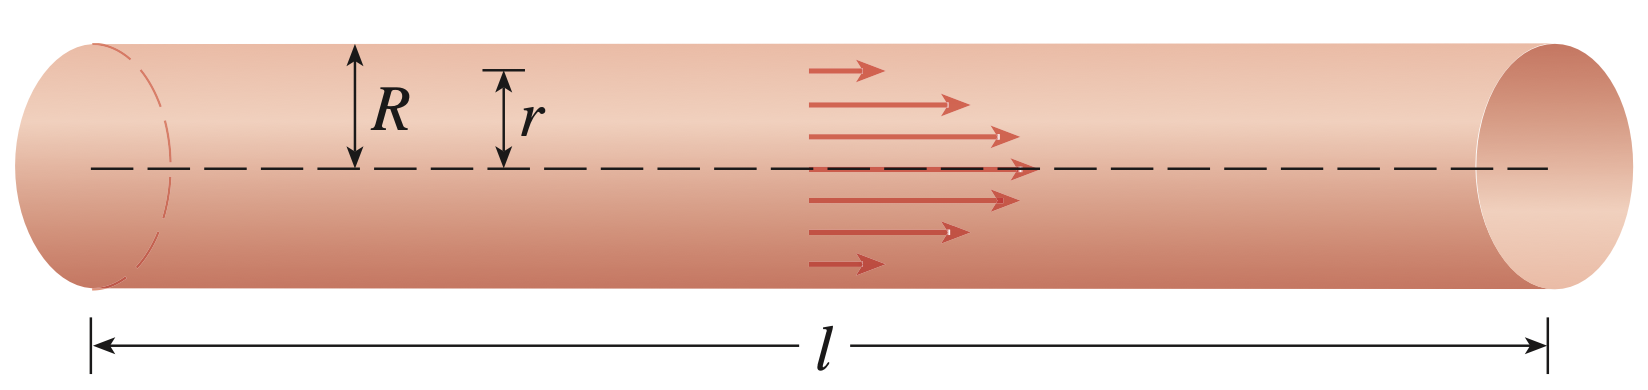
\includegraphics[scale=0.4]{chapter001/figures/fig006}
    \caption{Blood Vessel}
    \label{fig:Fig6}
\end{figure}

\begin{flushleft}
	Because of friction at the walls of the tube, the velocity v of the blood is greatest along the central axis of the tube and decreases as the distance r from the axis increases until v becomes 0 at the wall. The relationship between v and r is given by the law of laminar flow, which was experimentally derived by the French physicist Jean Léonard Marie Poiseuille in 1838. This law states that:
\end{flushleft}

\begin{equation}
	\label{eq:5}
	v = \frac{P}{4 \eta L}(R^2 - r^2)
\end{equation}
where\\
$\eta$ : viscosity of the blood.\\
$P$    : pressure difference between the ends of the blood vessel.\\
$L$    : length of the blood vessel.\\
$R$    : radius of the blood vessel.\\
$r$    : radius of the specific point inside the blood vessel that we want to know

\begin{flushleft}
If $P$ and $l$ are constant, then $v$ is a function of r with domain $[0, R]$. The average rate of change of the velocity as we move from $r=r_1$ outward to $r = r_2$ is given by
\end{flushleft}
$$
\frac{\Delta v}{\Delta r} = \frac{v(r_2) - v(r_1)}{r_2 - r_1}
$$
and if we let $\Delta r \rightarrow 0$, we obtain the velocity gradient, that is

\begin{equation}
	\label{eq:6}
	velocity\ gradient = \lim_{\Delta r \to 0} \frac{\Delta v}{\Delta r} = \frac{dv}{dr}
\end{equation}
Because $P$, $\eta$ and $L$ are constant, then we have
$$
	\frac{dv}{dr} = - \frac{Pr}{2 \eta L}
$$
Given $\eta=0.027$, $R=0.008cm$, $L=2cm$, and $P=4000 \ dynes/cm^2$, which gives
$$
    v = \frac{4000}{4\cdot(0.027)\cdot2} (0.000064 - r^2) \approx 1.85 \cdot 10^4(6.4 \cdot 10^{-5} - r^2)
$$
At $r=0.002cm$ the blood is flowing at a speed of
$$
    v(0.002) \approx 1.85 \cdot 10^4 (64 \cdot 10^{-6} - 4 \cdot 10^{-6}) = 1.11\ cm/s
$$
and the velocity gradient at that point is
$$
    \frac{dv}{dr}=-\frac{4000(0.002)}{2(0.027)2} \approx -74 (cm/s)/cm
$$
To get a feeling for what this statement means, let’s change our units from centimeters to micrometers ($1cm=10000 \mu m$). Then the radius of the artery is $80 \mu m$. The velocity at the center axis is $11,850 \mu m/s$, which decrease to $11,110 \mu m/s$ at a distance of $r=20 \mu m$. The fact that $\frac{dv}{dr}=-74(\mu m/s)/\mu m$ means that, when $r=20\mu m$, the velocity is decreasing at a rate of about $74\mu m/s$ for each micrometer that we proceed away from the center.

\subsection{Economics Cost Function}
Suppose $C(x)$ is the total cost that a company incurs in producing $x$ units of a certain commodity. The function $C$ is called a \textbf{cost function}. If the number of items produced is increased from $x_1$ to $x_2$, then the additional cost is $\Delta C=C(x_2) - C(x_1)$, and the average rate of change of the cost is 
$$
    \frac{\Delta c}{\Delta x}=\frac{C(x_2) - C(x_1)}{x_2 - x_1} = \frac{C(x_1 + \Delta x) - C(x_1)}{\Delta x}
$$
The limit of this quantity as $\Delta x \rightarrow 0$, that is, the instantaneous rate of change of cost with respect to the number of items produced, is called the \textbf{marginal cost} by economist:
$$
    marginal\ cost = \lim_{\Delta x \to 0} \frac{\Delta C}{\Delta x} = \frac{dC}{dx}
$$
Taking $\Delta x = 1$ and $n$ large (so that $\Delta x$ is small compared to $n$), we have
$$
    C'(n) \approx C(n+1) - C(n)
$$
Thus the marginal cost of producing $n$ units is approximately equal to the cost of the producing one more unit [the (n + 1)st unit].\\
It is often appropriate to represent a total cost function by a polynomial
$$
    C(x) = a + bx + cx^2 + dx^3
$$
where a represents the overhead cost (rent, heat, maintenance) and the other terms represent the cost of raw materials, labor, and so on.
For instance, suppose a company has estimated that the cost (in dollars) of producing $x$ items is
$$
    C(x) = 10000 + 5x + 0.01x^2
$$
Then the marginal cost function is
$$
    C'(x) = 5 + 0.02x
$$
The marginal cost at the production level of 500 items is
$$
    C'(500) = 5 + 0.02(500) = \$15/item
$$
This gives the rate at which costs are increasing with respect to the production level when $x=500$ and predicts the cost of the 501st item.\\
The actual cost of producing the 501st item is
$$
    C(501) - C(500) = \$15.01 \approx C'(500)
$$


\chapter{Directional Derivatives and Gradient Vector}

\section{Directional Derivatives}
\begin{definition}
    The \textbf{directional derivative} of $f$ at $(x_0, y_0) $ in the direction of a unit vector $\textbf{u}=<a, b>$ is
    \begin{equation}
        D_uf(x_0, y_0)= \lim_{h \to 0} \frac{f(x_0 + ha, y_0 + hb) - f(x_0, y_0}{h}
    \end{equation}
    if this limit exists.
\end{definition}

\begin{figure}[h]
    \centering
    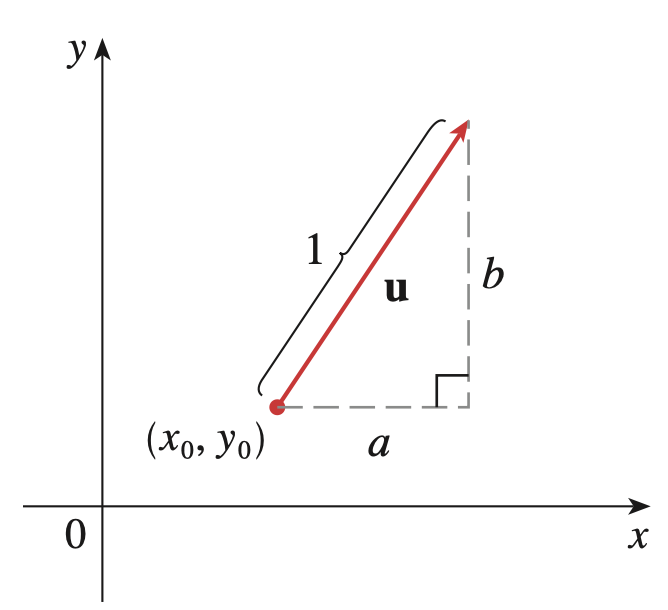
\includegraphics[scale=0.6]{chapter002/figures/fig002}
    \caption{Unit Vector}
    \label{fig:Unit Vector}
\end{figure}

\begin{figure}[h]
    \centering
    \cite{calculus}
    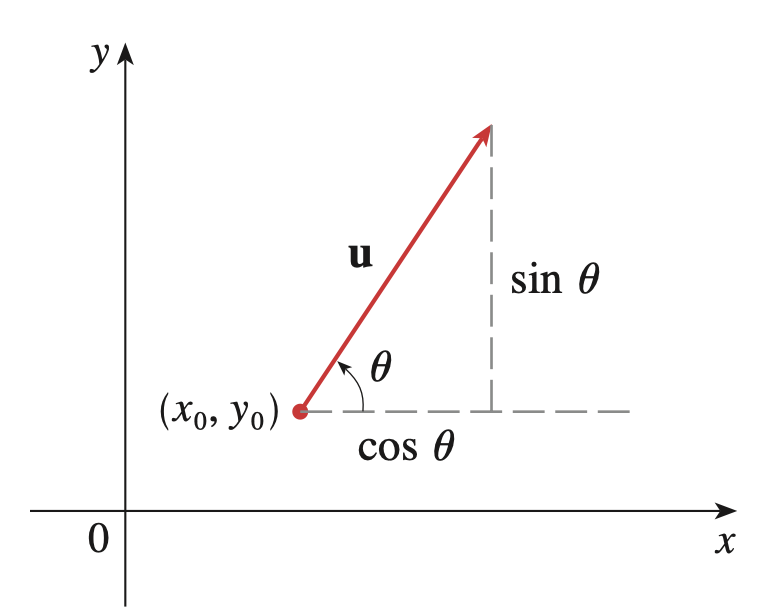
\includegraphics[scale=0.6]{chapter002/figures/fig003}
    \caption{Unit Vector}
    \label{fig:Unit Vector}
\end{figure}

\begin{figure}[h]
    \centering
    \cite{calculus}
    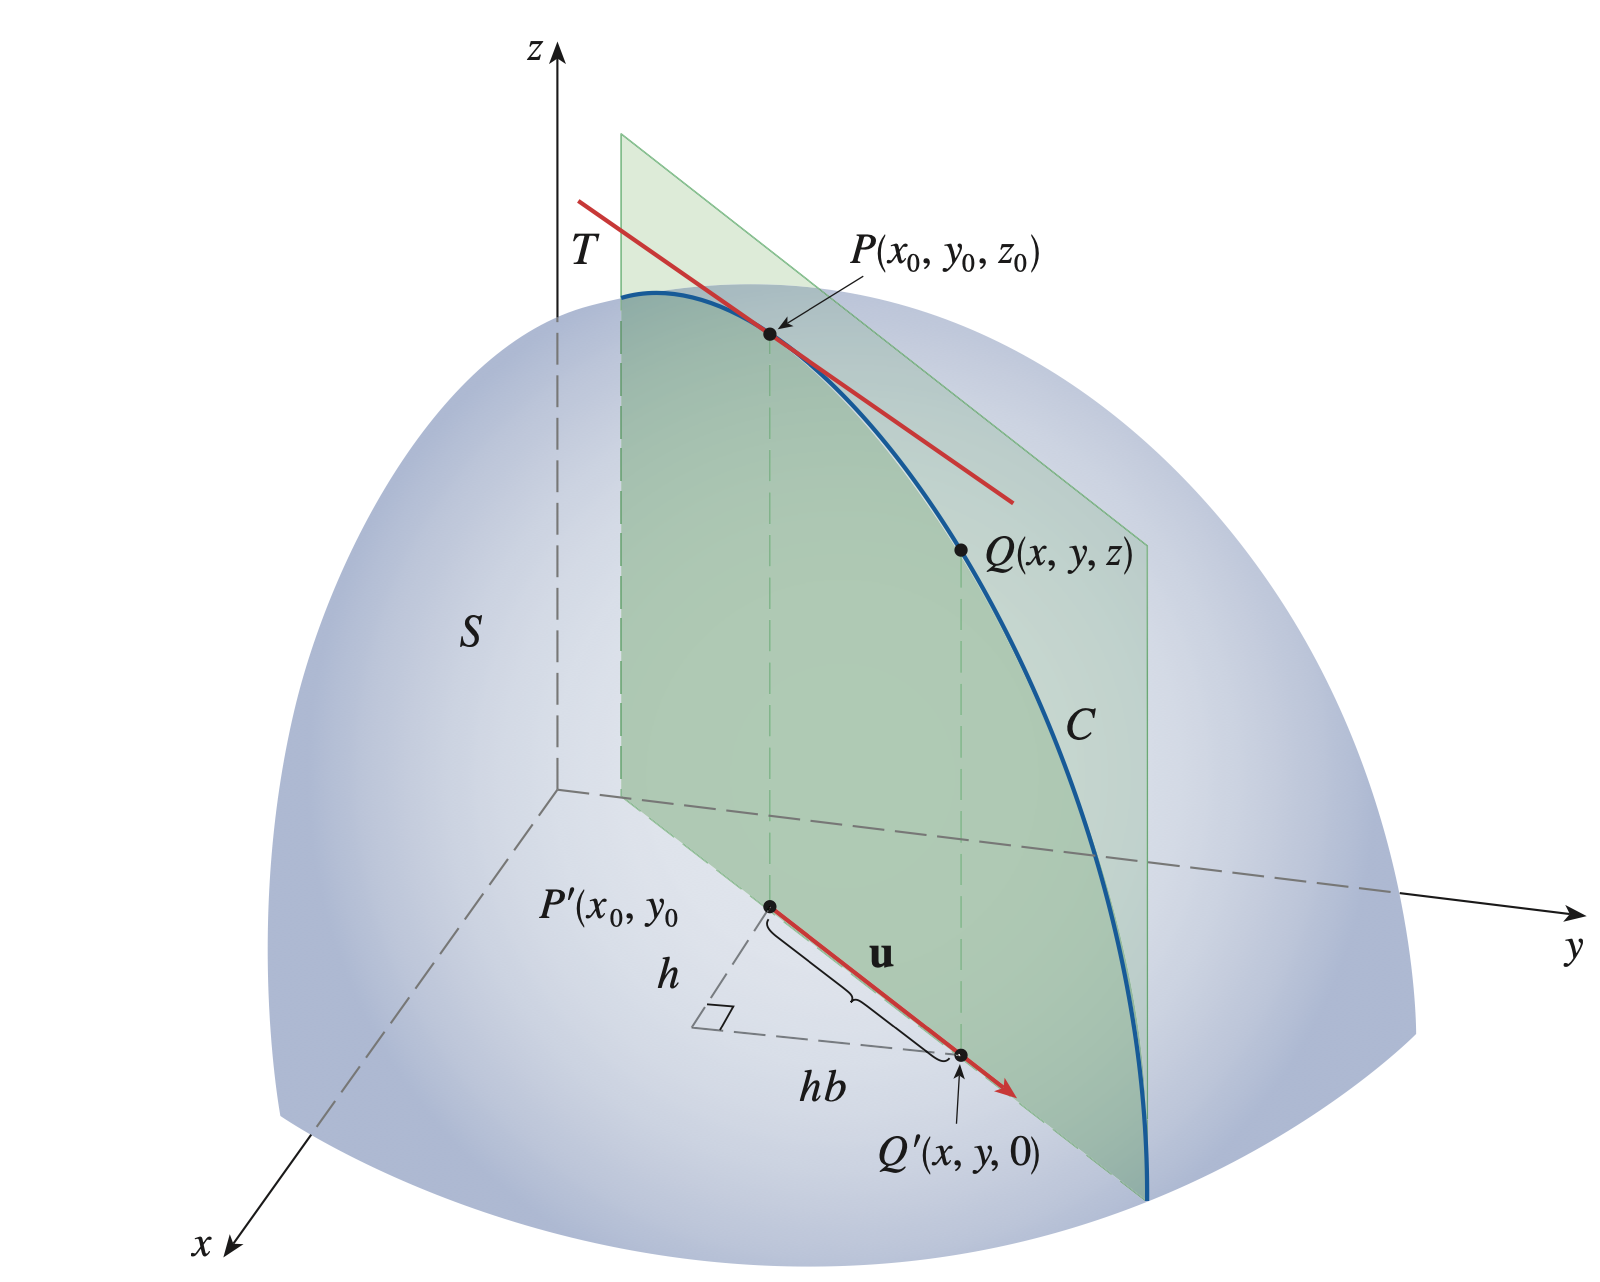
\includegraphics[scale=0.5]{chapter002/figures/fig001}
    \caption{Directional Derivative}
    \label{fig:Directional Derivative}
\end{figure}

\begin{theorem}
    If $f$ is a differentiable function of $x$ and $y$, then $f$ has a directional derivative in the direction of any unit vector $\textbf{u} = <a, b>$ and
    \begin{equation}
        D_uf(x, y) = f_x(x, y)a + f_y(x, y)b
    \end{equation}
\end{theorem}

\subsubsection{Proof}
If we define a function $g$ of the single variable $h$ by
$$
    g(h) = f(x_0 + ha, y_0 + hb)
$$
then, by the definition of a derivative, we have
$$
    g'(0) = \lim_{h \to 0}\frac{g(h) - g(0)}{h} = \lim_{h \to 0}\frac{f(x_0 + ha, y_0 + hb) - f(x_0, y_0)}{h} = D_uf(x_0, y_0)
$$
let,

\begin{tabularx}{\linewidth}{@{}XX@{}}
    $
        x = x_0 + ha
    $
    &
    $
        y = y_0 + hb
    $
\end{tabularx}

thus,
$$
    g(h) = f(x, y)
$$
$$
    g'(h) = \frac{\partial f}{\partial x}\frac{\partial x}{\partial h} + \frac{\partial f}{\partial y}\frac{\partial y}{\partial h} = f_x(x, y)a + f_y(x, y)b
$$
since,

\begin{tabularx}{\linewidth}{@{}XX@{}}
$$
    \frac{\partial x}{\partial h}=\frac{\partial (x_0 + ha)}{\partial h}=a
$$
&
$$
    \frac{\partial y}{\partial h}=\frac{\partial (y_0 + hb)}{\partial h}=b
$$
\end{tabularx}

\begin{theorem}
    If the unit vector $\textbf{u}$ makes an angle $\theta$ with the positive x-axis, then we can write $\textbf{u}=<\cos \theta, \sin \theta>$, then
    \begin{equation}
        \label{eq:Directional Derivative}
        D_uf(x, y)=f_x(x, y)\cos \theta + f_y(x, y) \sin \theta
    \end{equation}
\end{theorem}

\section{The Gradient Vector}
\begin{definition}
    The directional derivative of a differentiable function can be written as the dot product of two vectors.
    \begin{equation}
        D_uf(x, y)=f_x(x, y)a + f_y(x, y)b=<f_x(x, y), f_y(x, y)> \cdot <a, b> = <f_x(x, y), f_y(x, y)> \cdot u
    \end{equation}
\end{definition}
$<f_x(x, y), f_y(x, y)>$ is called gradient vector and noted as $\nabla f$

\subsection{Example 1}
Find the directional derivative of the function $f(x, y)=x^2y^3-4y$ at the point $(2, -1)$ in the direction of the vector $\vec{v}=2\vec{i} + 5\vec{j}$

\subsubsection{Solution}
$$
    \nabla f(x, y)=<f_x(x, y), f_y(x, y)>=<2xy^3, 3x^2y^2 - 4>
$$
$$
    \nabla f(2, -1)=<-4, 8>
$$
Note that $v$ is not a unit vector, but since $|\vec{v}|=\sqrt{29}$, the unit vector in the direction of $\vec{v}$ is
$$
    \vec{u}=\frac{\vec{v}}{|\vec{v}|}=\frac{2}{\sqrt{29}}\vec{i} + \frac{5}{\sqrt{29}}\vec{j}
$$
Therefore, we have
$$
    D_uf(2, -1)=\nabla f(2, -1) \cdot \vec{u} = (-4 \vec{i} + 8 \vec{j}) \cdot (\frac{2}{\sqrt{29}}\vec{i} + \frac{5}{\sqrt{29}}\vec{j})=\frac{-4 \cdot 2 + 8 \cdot 5}{\sqrt{29}} = \frac{32}{\sqrt{29}}
$$

\begin{figure}[h]
    \centering
    \cite{calculus}
    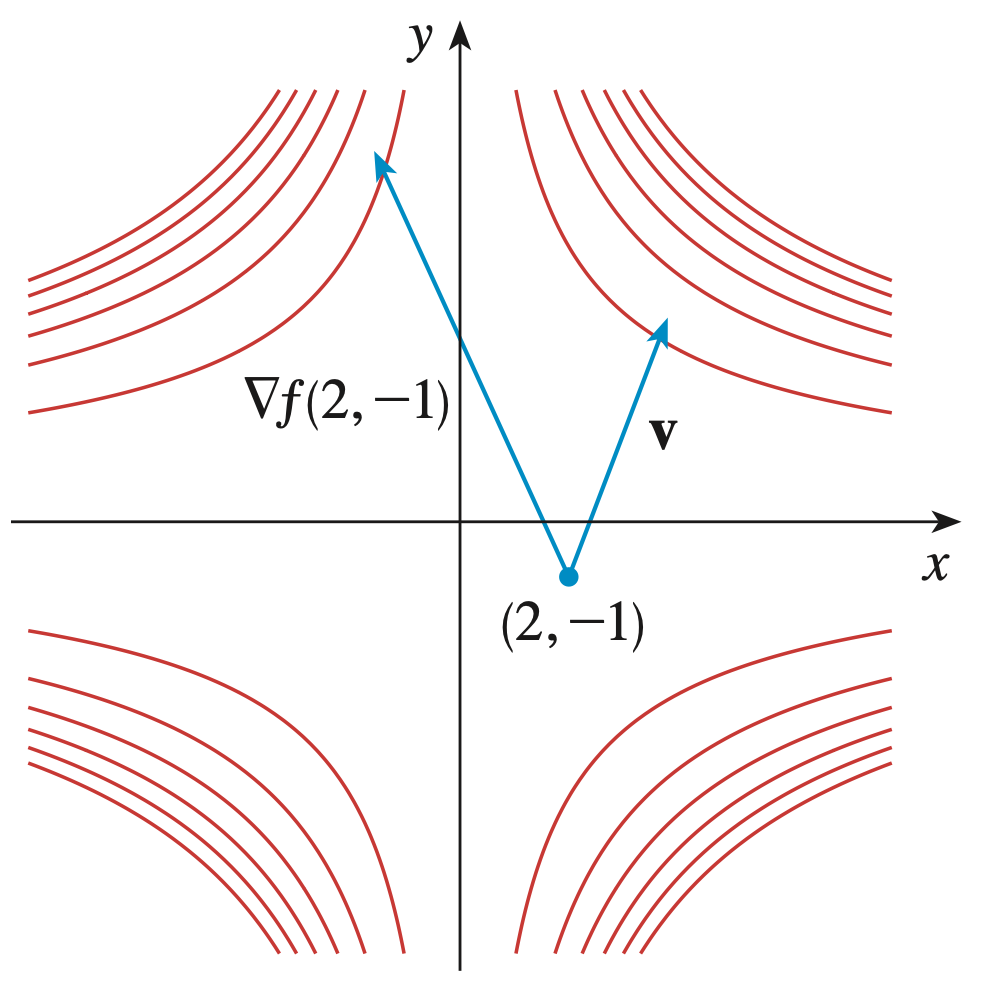
\includegraphics[scale=0.6]{chapter002/figures/fig004}
    \caption{Gradient Vector}
    \label{fig:Gradient Vector}
\end{figure}

\section{Maximizing the Directional Derivative}

\begin{theorem}
    Suppose $f$ is a differentiable function of two or three variables. The maximum value of the directional derivative $D_uf(x)$ is $| \nabla f(x)|$ and it occurs when $\vec{u}$ has the same direction as the gradient vector $\nabla f(x)$
\end{theorem}
\subsubsection{Proof}
\begin{equation}
    D_uf=\nabla f \cdot \vec{u}=|\nabla f||\vec{u}|\cos \theta = |\nabla f| \cos \theta
\end{equation}
where $\theta$ is the angle between $\nabla f$ and $\vec{u}$. The maximum value of $\cos \theta$ is 1 and this occurs when $\theta=0$. Therefore the maximum value of $D_uf$ is  $|\nabla f|$ and it occurs when $\theta=0$, that is, when $\vec{u}$ has the same direction as $\nabla f$.

\subsection{Example 2}
(a) If $f(x, y)=xe^y$, find the rate of change of $f$ at the point $P(2, 0)$ in the direction from $P$ to $Q(\frac{1}{2}, 2)$.
(b) In what direction does $f$ have the maximum rate of change? What is this maximum rate of change?

\subsubsection{Solution}
$$
    \nabla f(x, y)=<f_x, f_y>=<e^y, xe^y>
$$
$$
    \nabla f(2, 0)=<1, 2>
$$
(a)
The unit vector in the direction of $\vec{PQ}=<-\frac{3}{2}, 2>$ is $\vec{u}=<-\frac{3}{5}, \frac{4}{5}>$, so the rate of change of $f$ in the direction from $P$ to $Q$ is
$$
    D_uf(2, 0)=\nabla f(2, 0) \cdot \vec{u} = <1, 2> \cdot <-\frac{3}{5}, \frac{4}{5}> = 1
$$ 
(b)
$f$ increases fastest in the direction of the gradient vector $\nabla f(2, 0)=<1, 2>$. The maximum rate of change is
$$
    |\nabla f(2, 0)| = |<1, 2>| = \sqrt{5}
$$
\begin{figure}[h]
    \centering
    \cite{calculus}
    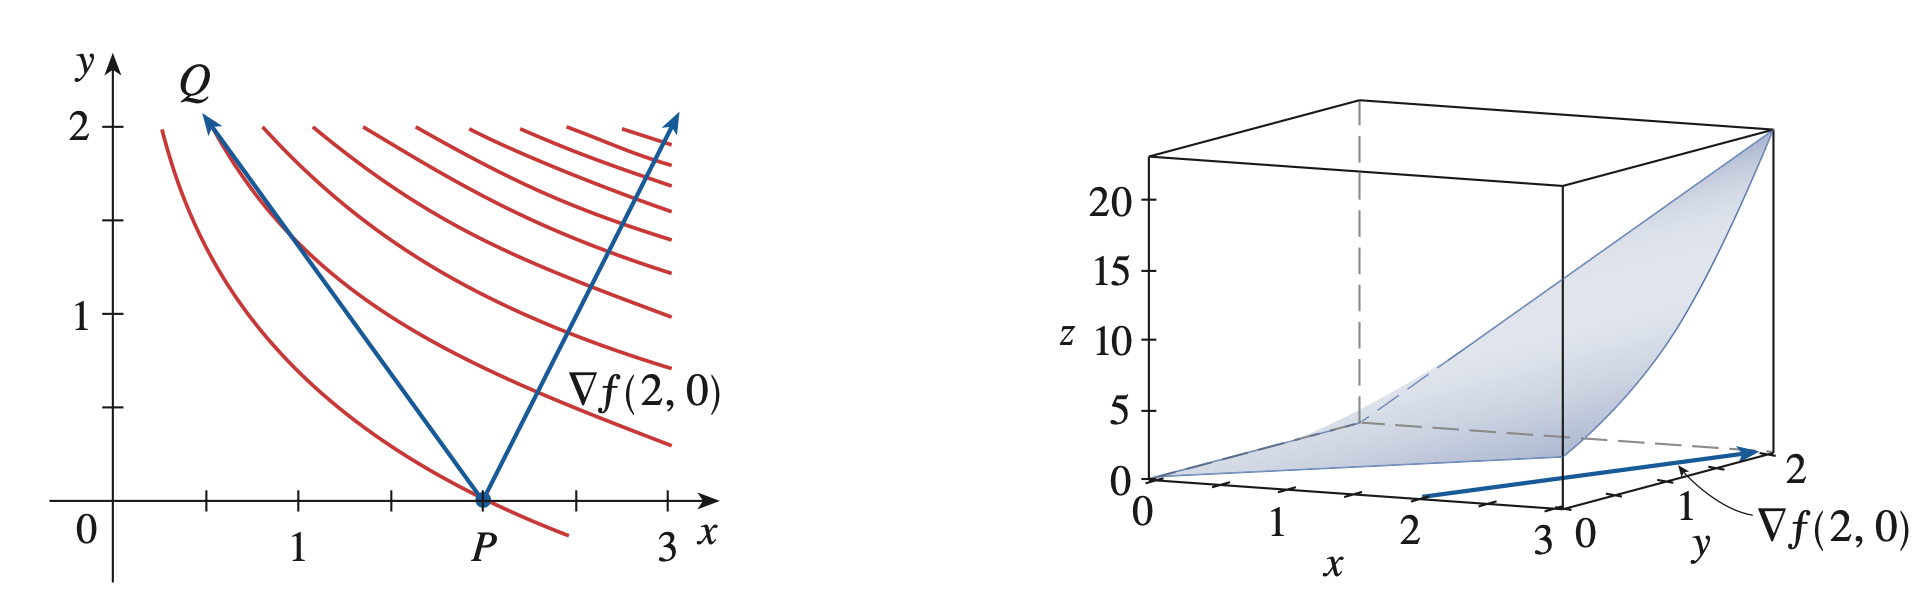
\includegraphics[scale=0.45]{chapter002/figures/fig005}
    \caption{Gradient Vector Example}
    \label{fig:Gradient Vector Example}
\end{figure}

\section{Applications}
\subsection{Snake reversals and stripes}
In a study of the survivorship of juvenile garter snakes, a researcher arrived at the model (\cite{calculus}, page 614)
$$
    F = 4.2 + 0.008R + 0.102S + 0.017R^2 - 0.034S^2 - 0.268RS
$$
where $F$ is a measure of the fitness of the snake, $R$ measures the number of reversals of direction during flight from a predator, and $S$ measures the degree of stripedness in the color pattern of the snake. How does $F$ change when $R=3$ and $S=2$ if the phenotype changes so that $R$ and $S$ increased by equal amounts?

The gradient vector of $F$ is
$$
    \nabla F(R, S) = [F_R, F_S] = [0.008 + 0.034R - 0.268S, 0.102 - 0.068S - 0.268R]
$$
and when $R=3$ and $S=2$ this becomes
$$
    \nabla F(3, 2) = [-0.426, -0.838]
$$
We want the derivative in the direction halfway between $\vec{i}$ and $\vec{j}$, that is, in the direction $\vec{v}=[1, 1]$. The unit vector in this direction is $\vec{u}=(1/\sqrt{2})[1, 1]$, so the directional derivative is
$$
    D_{\vec{u}}F(3, 2)=\nabla F(3, 2) \cdot \vec{u}=[-0.426, -0.838] \cdot [\frac{1}{\sqrt{2}}, \frac{1}{\sqrt{2}}]
    \approx 0.894
$$
This means that the fitness function at (3, 2) decreases at a rate of 0.894 units when $R$ and $S$ increase by equal amount.
\chapter{Probability Theory}

\section{Random Variables}
Given a random variable $X$, one may generate other random variables by applying various transformations on $X$. As an example, Y is a \textbf{linear} function of $X$, of the form

\begin{equation}
    Y = g(x) = aX + b
\end{equation}

where $a$ and $b$ are given scalars.

If $Y = g(X)$ is a function of a random variable $X$, then $Y$ is also a random variable, since it provides a numerical value for each possible outcomes. This is because every outcome in the sample space defines a numerical value $x$ for $X$ and hence also the numerical value $y = g(x)$ for $Y$.

If $X$ is discrete with PMF $p_X$, then $Y$ is also discrete, and its PMF $p_Y$ can be calculated using the PMF of $p_X$. To obtain $p_Y(y)$ for any $y$, we add the probabilities of all value $x$ such that $g(x) = y$

\begin{equation}
    p_Y(y) = \sum_{x | g(x) = y} p_X(x)
\end{equation}



\section{Conditional Probability}

Imagine we have two boxes, one red and one blue, and in the red box we have 2 apples and 6 oranges, and in the blue box we have 3 apples and 1 orange.

Now suppose we randomly pick one of the boxes and from that box we randomly select an item of fruit.

Let us suppose that in so doing we pick the red box 40\% of the time and we pick the blue box 60\% of the time.

The identity of the box that will be chosen is a random variable, which we shall denote by $B$. This random variable can take one of two possible values, namely $r$ (red box) or $b$ (blue box).

The identity of the fruit is also a random variable and will be denoted by $F$.  It can take either of the values $a$ (apple) or $o$ (orange).

The probability of selecting the red box is $\frac{4}{10}$ and the probability of selecting the blue box is $\frac{6}{10}$. In other words, $p(B = r) = \frac{4}{10}$ and $p(B = b) = \frac{6}{10}$.

By definition, probabilities must lie in the interval $[0, 1]$. If the events are mutually exclusive and if they include all possible outcomes, then we see that the probabilities for those events must sum to one.

\begin{enumerate}
    \item What is the overall probability that the selection procedure will pick an apple?
    \item Given that we have chosen an orange, what is the probability that the box we chose was the blue one?
\end{enumerate}

\begin{figure}
    \centering
    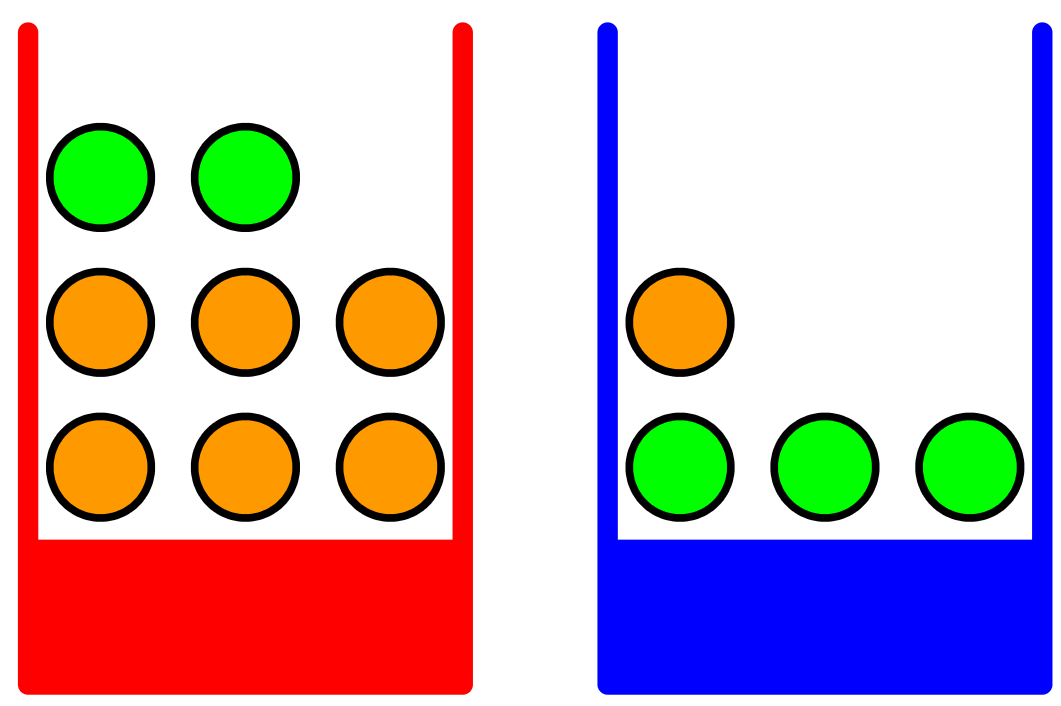
\includegraphics[width=5cm]{chapter008/figures/fig001.png}
    \caption{Line representation}
\end{figure}

We shall suppose that $X$ can take any of the values $x_i$ where $i = 1, ..., M$, and $Y$ can take the values $y_j$ where $j=1, ..., L$.

Consider a total of $N$ trials in which we sample both of the variables $X$ and $Y$, and let the number of such trials in which $X=x_i$ and $Y = y_j$ be $n_{ij}$.

Let the number of trials in which $X$ takes the value $x_i$ be denoted by $c_i$, and similarity let the number of trials in which $Y$ takes the value $y_j$ be denoted by $r_j$

The probability that $X$ will take the value $x_i$ and $Y$ will take the value $y_j$ is written $p(X = x_i, Y = y_j)$ and is called the \textbf{joint probability} of $X = x_i$ and $Y = y_j$, and hence

\begin{equation}
    p(X = x_i, Y = y_j) = \frac{n_{ij}}{N}
\end{equation}

Here we are implicitly considering the limit $N \rightarrow \infty$. Similarity, the probability that $X$ takes the value $x_i$ irrespective of the value of $Y$ is written as $p(X = x_i)$, so that

\begin{equation}
    p(X = x_i) = \frac{c_{ij}}{N}
\end{equation}

\begin{equation}
    p(X = x_i) = \sum_{j=1}^L p(X = x_i, Y = y_j)
\end{equation}

\begin{figure}
    \centering
    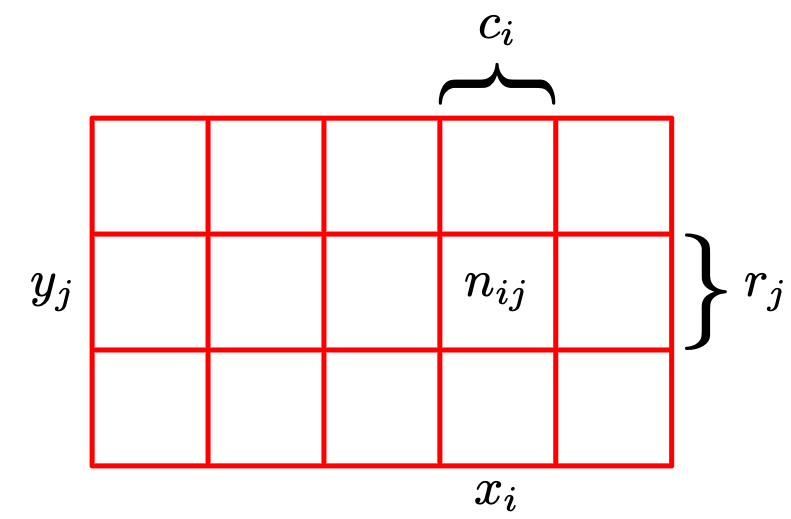
\includegraphics[width=5cm]{chapter008/figures/fig002.png}
    \caption{Join Probability}
\end{figure}

which is the sum rule of probability.  Note that $p(X=x_i)$ is sometimes called the $marginal$ probability, because it is obtained by marginalizing, or summing out.

If we consider only those instances for which $X = x_i$, then the fraction of such instances for which $Y=y_j$ is written $p(Y = y_j | X = x_i)$ and is called the \textbf{conditional} probability of $Y=y_j$ given $X=x_i$. It is obtained by finding the fraction of those points in column $i$ that fall in cell $i,j$ and hence is given by

\begin{equation}
    p(Y = y_j | X = x_i) = \frac{n_{ij}}{c_i}
\end{equation}

then,

\begin{equation}
    \begin{split}
        p(X = x_i, Y = y_j) & = \frac{n_{ij}}{N}\\
        & = \frac{n_{ij}}{c_i} \cdot \frac{c_i}{N}\\
        & = p(Y = y_j | X = x_i)p(X = x_i)
    \end{split}
\end{equation}

which is the \textbf{product rule} of probability.

Here $p(X, Y)$ is a joint probability and is verbalized as "the probability of $X$ and $Y$". The quantity $p(Y | X)$ is a conditional probability and is verbalized as "the probability of $Y$ given $X$", whereas the quantity $p(X)$ is marginal probability and is simply "the probability of $X$"

We have seen that the probabilities of selecting either the red or the blue boxes are given by

\begin{equation}
    p(B = r) = \frac{4}{10}\ \ \ 
    p(B = b) = \frac{6}{10}
\end{equation}

so, $p(B = r) + b(B = b) = 1$. 

Suppose that we pick a box at random, and it turns out to be the blue box. Then the probability of selecting an apple is just the fraction of apples in the blue box which is $3/4$, and so $p(F = a | B = b) = 3/4$. In fact,

$$
    p(F = a | B = r) = \frac{1}{4}\\
    p(F = o | B = r) = \frac{3}{4}\\
    p(F = a | B = b) = \frac{3}{4}\\
    p(F = o | B = b) = \frac{1}{4}\\
$$

and

\begin{equation}
    \begin{split}
        p(F = a) & = p(F = a | B = r)p(B = r) + p(F = a | B = b)p(B = b)\\
        & = \frac{1}{4} \times \frac{4}{10} + \frac{3}{4} \times \frac{6}{10} = \frac{11}{20}
    \end{split}
\end{equation}

if $p(X, Y) = p(X)p(Y)$, then $X$ and $Y$ are said to be independent. If each box contained the same fraction of apples and oranges, then $p(F|B) = P(F)$.


\section{Total Probability Theorem}
Let $A_1, ..., A_n$ be disjoint events that form a partition of the sample space and assume that $P(A_i) > 0$, for all $i$. Then, for any event B, we have

\begin{equation}
    \begin{split}
        P(B) & = P(A_1 \cap B) + ... + P(A_n \cap B)\\
        & = P(A_1)P(B | A_1) + ... + P(A_n)P(B | A_n)
    \end{split}
\end{equation}


\begin{equation}
    B = (A_1 \cap B) \cup ... \cup (A_n \cap B)
\end{equation}

Using the additivity axiom, it follows that

\begin{equation}
    P(B) = P(A_1 \cap B) + ... + P(A_n \cap B)
\end{equation}

by the definition of conditional probability, we have
\begin{equation}
    P(A_i \cap B) = P(A_i)P(B | A_i)
\end{equation}

then,
\begin{equation}
   P(B) = P(A_1)P(B | A_1) + ... + P(A_n)P(B | A_n)
\end{equation}


\section{Bayes' Theorem}

\begin{equation}
    p(Y|X) = \frac{p(X|Y)p(Y)}{p(X)}
\end{equation}

where

\begin{equation}
    p(X) = \sum_{Y} p(X|Y)p(Y)
\end{equation}

Suppose we are told that a piece of fruit has been selected and it is an orange, and we would like to know which box it came from. This requires that we evaluate the probability distribution over boxes conditioned on the identity of the fruit.

We can solve the problem of reversing the conditional probability by using Bayes's theorem to give

\begin{equation}
    p(B = r | F = 0) = \frac{p(F = o | B = r)p(B = r)}{p(F = o)} = \frac{3}{4} \times \frac{4}{10} \times \frac{20}{9} = \frac{2}{3}
\end{equation}

If we had been asked which box had been chosen before being told the identity of the selected item of fruit, then the most complete information we have available is provided by the probability $p(B)$ which is called \textbf{prior probability} because it is the probability available \textbf{before} we observe the identity of the fruit. Once we are told that the fruit is an orange, we can then use Bayes' theorem to compute the probability $p(B | F)$, which is shall call the \textbf{posterior probability}, because it is the probability obtained  \textbf{after} we have observed F.

Let $A_1, A_2, ..., A_n$ be disjoint events that form a partition of the sample space, and assume that $P(A_i) > 0$, for all $i$. Then, for any event B such that $P(B) > 0$, we have

\begin{equation}
    \begin{split}
        P(A_i | B) & = \frac{P(A_i)P(B | A_i)}{P(B)}\\
        & = \frac{P(A_i)P(B | A_i)}{P(A_1)P(B | A_1) + ... + P(A_n)P(B|A_n)}
    \end{split}
\end{equation}

\section{Exercise}

\subsection{Exercise 1}
You enter a chess tournament where your probability of winning a game is $0.3$ against half the players (call them type 1), 0.4 against a quarter of the players (call them type 2), and 0.5 against the remaining quarter of the players (call them type 3). You play a game against a randomly chosen opponent. What is the probability of wining?

Let $A_i$ be the \textbf{event of playing with} an opponent of type $i$. We have
$$
    P(A_1) = 0.5, P(A_2) = 0.25, P(A_3) = 0.25
$$

Also, let B be the event of winning. We have

$$
    P(B | A_1) = 0.3, P(B | A_2) = 0.4, P(B | A_3) = 0.5
$$

Thus, the probability of winning is

\begin{equation}
    \begin{split}
        P(B) & = P(A_1)P(B | A_1) + P(A_2)P(B|A_2) + P(A_3)P(B|A_3)\\
        & = 0.5 \cdot 0.3 + 0.25 \cdot 0.4 + 0.25 \cdot 0.5\\
        & = 0.375
    \end{split}
\end{equation}

\section{Expectations}

One of the most important operations involving probabilities is that of finding weighted averages of functions. The average value of some function $f(x)$ under a probability distribution $p(x)$ is called the \textbf{expectation} of $f(x)$ and will be denoted by $\mathbb{E}[f]$

\begin{equation}
    \mathbb{E}[f] = \sum_x p(x)f(x)
\end{equation}

so that the average is weighted by the relative probabilities of the different values of $x$.

\begin{equation}
    \mathbb{E}[f] = \int p(x)f(x)dx
\end{equation}

In either case, if we are given a finite number $N$ of points drawn from the probability distribution or probability density, then the expectation can be approximated as a finite sum over these points. 

\begin{equation}
       \mathbb{E}[f] \simeq \frac{1}{N}\sum_{n=1}^N f(x_n) 
\end{equation}

The approximation becomes exact in the limit $N \rightarrow \infty$.

\section{Conditional Expectation}

\begin{equation}
    \mathbb{E}[f | y] = \sum_x p(x | y)f(x)
\end{equation}

\section{Properties of Mean and Variance}

Given $a$ and $b$ are scalars,

\begin{equation}
    \begin{split}
        \mathbb{E}[aX + b] & = \sum_x (ax + b)p_X(x)\\
         & = a \sum_x xp_X(x) + b\sum_x p_X(x)\\
         & = a \mathbb{E}[X] + b
    \end{split}
\end{equation}

because $\sum_x p_X(x) = 1$

\section{Variance}

\begin{equation}
    \begin{split}
        var[X] & = \mathbb{E}[(X - \mu])^2]\\
        & = \sum_x (x - \mu)^2p_X(x)\\
        & = \sum_x(x^2 -2x\mu + \mu^2)p_X(x)\\
        & = \sum_xx^2p_X(x) - \sum_x 2x \mu p_X(x) + \sum_x \mu^2p_X(x)\\
        & = \sum_xx^2p_X(x) - 2\mu \sum_x x p_X(x) + \mu^2\sum_x p_X(x)\\
        & = E[X^2] - 2\mu^2 + \mu^2\\
        & = E[X^2] - \mu^2
    \end{split}
\end{equation}

because $\mu = \mathbb{E}[f(x)$ is just a number and $\sum_x p_X(x) = 1$.

The variance of f(x) provides a measure of how much variability there is in $f(x)$ around its mean value $\mathbb{E}$.

\section{Covariance}
\begin{equation}
    \begin{split}
        cov[x, y] & = \mathbb{E}_{x, y}[\{x - \mathbb{E}[x]\}\{y - \mathbb{E}[y]\}]\\
        & = \mathbb{E}_{x, y}[xy - x\mathbb{E}[y] - y\mathbb{E}[x] + \mathbb{E}[x]\mathbb{E}[y]]\\
        & = \mathbb{E}_{x, y}[xy] - \mathbb{E}_{x, y}[x\mathbb{E}[y]] - \mathbb{E}_{x, y}[y\mathbb{E}[x]] +  \mathbb{E}_{x, y}[\mathbb{E}[x]\mathbb{E}[y]]\\
        & = \mathbb{E}_{x, y}[xy] - \mathbb{E}[y]\mathbb{E}_{x, y}[x] - \mathbb{E}[x]\mathbb{E}_{x, y}[y] + \mathbb{E}[x]\mathbb{E}[y]\\
        & = \mathbb{E}_{x, y}[xy] - 2\mathbb{E}[x]\mathbb{E}[y] + \mathbb{E}[x]\mathbb{E}[y]\\
        & = \mathbb{E}_{x, y}[xy] - \mathbb{E}[x]\mathbb{E}[y]
    \end{split}
\end{equation}

if $x$ and $y$ are independent, then their covariance vanishes.

In the case of two vectors of random variables $x$ and $y$, the covariance is a matrix

\begin{equation}
    \begin{split}
        cov[x, y] & = \mathbb{E}_{x, y}[\{x - \mathbb{E}[x]\}\{y^T -  \mathbb{E}[y^T]\}]\\
        & = \mathbb{E}_{x, y}[xy^T] - \mathbb{E}[x]\mathbb{E}[y^T]
    \end{split}
\end{equation}

Note that each data point is a vector, then average of multiple vectors is also a vector.

\section{The Gaussian Distribution}
It is also called \textbf{normal} distribution. For the case of a single real-valued variable $x$, the Gaussian distribution is defined by

\begin{equation}
    \mathcal{N}(x | \mu, \sigma^2) = \frac{1}{(2\pi \sigma ^2)^{1/2}} e^{-\frac{1}{2\sigma^2}(x - \mu)^2}
\end{equation}

which is governed by two parameters: $\mu$, called \textbf{mean}, and $\sigma^2$, called the \textbf{variance}. The square root of the variance, given by $\sigma$, is called the \textbf{standard deviation}, and the reciprocal of the variance, written as $\beta = \frac{1}{\sigma^2}$, is called the precision.

The Gaussian distribution satisfies

\begin{equation}
    \mathcal{N}(x | \mu, \sigma^2) > 0
\end{equation}

Let 

\begin{equation}
    I = \int_{- \infty}^{\infty} exp(- \frac{1}{2 \sigma^2}x^2)dx 
\end{equation}

then,

\begin{equation}
    \begin{split}
        I^2 & = \int_{- \infty}^{\infty} \int_{- \infty}^{\infty} exp(- \frac{1}{2 \sigma^2}x^2) exp(- \frac{1}{2 \sigma^2}y^2)dxdy\\
        & = \int_{- \infty}^{\infty} \int_{- \infty}^{\infty} exp(- \frac{1}{2 \sigma^2}x^2 - \frac{1}{2 \sigma^2}y^2 )dxdy\\
        & = \int_{- \infty}^{\infty} \int_{- \infty}^{\infty} exp(- \frac{1}{2 \sigma^2}(x^2 + y^2) )dxdy\\
    \end{split} 
\end{equation}

Let
$$
    x = rcos \theta, y = r sin \theta
$$
 
then,

\begin{align*}
    \frac{\partial(x, y)}{\partial (r, \theta)} = 
    \begin{vmatrix}
        \frac{\partial x}{\partial r} & \frac{\partial x}{\partial \theta}\\
        \frac{\partial y}{\partial r} & \frac{\partial y}{\partial \theta}
    \end{vmatrix}dr d\theta
    =
    \begin{vmatrix}
        \cos \theta & -r\sin \theta\\
        \sin \theta & r \cos \theta
    \end{vmatrix} dr d \theta = 
    r (\cos \theta)^2 + r (\sin \theta)^2drd \theta = rdrd\theta
\end{align*}

based on the fact:

\begin{equation}
    \begin{split}
        \int_{- \infty}^{\infty} exp(-\frac{r^2}{2\sigma^2})rdr
    \end{split}
\end{equation}

let $u = -\frac{r^2}{2\sigma^2}$, then

\begin{equation}
    du = -\frac{r}{\sigma^2}dr \Leftrightarrow -\sigma^2du = rdr
\end{equation}

then,

\begin{equation}
    \begin{split}
        \int_{- \infty}^{\infty} exp(-\frac{r^2}{2\sigma^2})rdr = -\sigma^2\int_{- \infty}^{\infty} exp(u)du = - \sigma^2 exp(u) |_0^{+\infty} = - \sigma^2 exp(-\frac{r^2}{2\sigma^2}) |_0^{+\infty}
    \end{split}
\end{equation}

because

$$
    exp(-\frac{r^2}{2\sigma^2}) = e^{-\frac{r^2}{2\sigma^2}} = \frac{1}{e^{\frac{r^2}{2\sigma^2}}} = 0 \ when\ r \rightarrow \infty
$$

thus

$$
    - \sigma^2 exp(-\frac{r^2}{2\sigma^2}) |_0^{+\infty} = -\sigma^2(0 - 1) = \sigma^2
$$

Note that in the trigonometry circle, the radius=1 and $cos \theta = r$, then

\begin{equation}
    \begin{split}
        y & = rsin\theta\\
        \Leftrightarrow dy & = sin \theta dr\\
        \Leftrightarrow dxdy & = cos \theta drd\theta\\
        \Leftrightarrow dxdy & = r drd\theta
    \end{split}
\end{equation}

\begin{equation}
    \begin{split}
        I^2 & = \int_{0}^{2 \pi} \int_{- \infty}^{\infty} exp(- \frac{1}{2 \sigma^2}(x^2 + y^2) )dxdy\\
        & = \int_{0}^{2 \pi} \int_{- \infty}^{\infty} exp(- \frac{1}{2 \sigma^2}r^2 )r drd\theta\\
        & = \int_{0}^{2 \pi} \sigma^2 d\theta\\
        & = \theta \sigma^2 |_{0}^{2\pi} = 2 \pi \sigma^2\\
        \Leftrightarrow I & = \sqrt{2 \pi}\sigma
    \end{split}
\end{equation}

Finally, let $y = x - \mu \Leftrightarrow dy = dx$

\begin{equation}
    \begin{split}
        \int_{- \infty}^{\infty} \mathcal{N}(x | \mu, \sigma^2)dx & = \int_{- \infty}^{\infty} \frac{1}{(2\pi \sigma ^2)^{1/2}} e^{-\frac{1}{2\sigma^2}(x - \mu)^2}dx\\
        & = \int_{- \infty}^{\infty} \frac{1}{(2\pi \sigma ^2)^{1/2}} e^{-\frac{1}{2\sigma^2}y^2}dy\\
        & = \frac{1}{(2\pi \sigma ^2)^{1/2}} \int_{- \infty}^{\infty} e^{-\frac{1}{2\sigma^2}y^2}dy\\
        & = \frac{I}{(2\pi \sigma ^2)^{1/2}}\\
        & = 1
    \end{split}
\end{equation}

Because the parameter $\mu$ represents the average value of $x$ under the distribution, it is referred as the mean

\begin{equation}
    \mathbb{E}[x] = \int_{- \infty}^{\infty} \mathcal{N}(x | \mu, \sigma^2)xdx = \mu
\end{equation}

To proof that, we need to know that

\begin{align}
    \begin{split}
        \int_{-a}^{a} f(x)dx & = \int_{-a}^{0} f(x)dx + \int_{0}^{a} f(x)dx\\
        & = - \int_{0}^{-a} f(x)dx + \int_{0}^{a} f(x)dx
    \end{split}
\end{align}

Let $u = -x$, then $du = -dx$ and $x = -a$, then $u = a$. Thus,

\begin{align}
    \begin{split}
        - \int_{0}^{-a} f(x)dx & = - \int_{0}^{a}  f(-u)(-du)\\
        & = \int_{0}^{a} f(-u)du
    \end{split}
\end{align}

In other words,

\begin{align}
    \begin{split}
        \int_{-a}^{a} f(x)dx & = \int_{0}^{a}  f(-u)(du) + \int_{0}^{a} f(x)dx\\
    \end{split}
\end{align}

If $f$ is odd, then $f(-u) = -f(u)$

\begin{align}
    \begin{split}
        \int_{-a}^{a} f(x)dx & = -\int_{0}^{a}  f(u)(du) + \int_{0}^{a} f(x)dx\\
        & = 0
    \end{split}
\end{align}

So we have,

\begin{align}
    \begin{split}
        \mathbb{E}[x] & = \int_{- \infty}^{\infty} \mathcal{N}(x | \mu, \sigma^2)xdx\\
        & = \int_{- \infty}^{\infty} \frac{1}{(2\pi \sigma ^2)^{1/2}} e^{-\frac{1}{2\sigma^2}(x - \mu)^2}xdx
    \end{split}
\end{align}

Let $y = x - \mu$,  then $x = y + \mu$ and $dy = dx$. We have

\begin{align}
    \begin{split}
        \mathbb{E}[x] & = \int_{- \infty}^{\infty} \mathcal{N}(x | \mu, \sigma^2)xdx\\
        & = \int_{- \infty}^{\infty} \frac{1}{(2\pi \sigma ^2)^{1/2}} e^{-\frac{1}{2\sigma^2}(y)^2}(y + \mu)dy\\
        & = \int_{- \infty}^{\infty} \frac{1}{(2\pi \sigma ^2)^{1/2}} e^{-\frac{1}{2\sigma^2}(y)^2}ydy + \int_{- \infty}^{\infty} \frac{1}{(2\pi \sigma ^2)^{1/2}} e^{-\frac{1}{2\sigma^2}(y)^2}\mu dy\\
    \end{split}
\end{align}

Because

\begin{align}
    \begin{split}
        \frac{1}{(2\pi \sigma ^2)^{1/2}} e^{-\frac{1}{2\sigma^2}(-y)^2}(-y) = - \frac{1}{(2\pi \sigma ^2)^{1/2}} e^{-\frac{1}{2\sigma^2}(y)^2}(y)
    \end{split}
\end{align}

so $\frac{1}{(2\pi \sigma ^2)^{1/2}} e^{-\frac{1}{2\sigma^2}(y)^2}y$ is an odd function. Thus,


$$
    \int_{- \infty}^{\infty} \frac{1}{(2\pi \sigma ^2)^{1/2}} e^{-\frac{1}{2\sigma^2}(y)^2}ydy = 0
$$

We have

$$
    \int_{- \infty}^{\infty} \frac{1}{(2\pi \sigma ^2)^{1/2}} e^{-\frac{1}{2\sigma^2}(y)^2}dy = 1
$$
so,

\begin{equation}
    \mathbb{E}[x] = \int_{- \infty}^{\infty} \mathcal{N}(x | \mu, \sigma^2)xdx = \mu
\end{equation}

Next,

\begin{align}
    \begin{split}
        \mathbb{E}[(x - \mu)^2] & = \int_{- \infty}^{\infty} (x - \mu)^2 \mathcal{N}(x | \mu, \sigma^2)dx\\
        & = \frac{1}{\sigma\sqrt{2\pi}}\int_{- \infty}^{\infty} (x - \mu)^2 exp(- \frac{1}{2 \sigma^2}(x - \mu)^2)dx
    \end{split}
\end{align}

Let
\begin{align}
        y = x - \mu \Leftrightarrow dy = dx  \qquad    x = y + \mu
\end{align}

so,

\begin{align}
    \begin{split}
        \mathbb{E}[(x - \mu)^2] & = \int_{- \infty}^{\infty} (x - \mu)^2 \mathcal{N}(x | \mu, \sigma^2)dx\\
        & = \frac{1}{\sigma\sqrt{2\pi}}\int_{- \infty}^{\infty} y^2 exp(- \frac{1}{2 \sigma^2}y^2)dx
    \end{split}
\end{align}

let

\begin{equation}
    \begin{cases}
      u & = y\\
      v & = - \sigma ^ 2 e^{- \frac{y^2}{2 \sigma^2}}\\
    \end{cases}
    \Leftrightarrow
    \begin{cases}
      du & = dy\\
      dv & = - \sigma ^ 2 (-\frac{2y}{2 \sigma ^2}) e^{- \frac{y^2}{2 \sigma^2}}dy\\
    \end{cases}
    \Leftrightarrow
    \begin{cases}
      du & = dy\\
      dv & = y e^{- \frac{y^2}{2 \sigma^2}}dy\\
    \end{cases}
\end{equation}

Applying Formula for Integration by Parts, we have
\begin{equation}
    \begin{split}
        \int u dv & = u v - \int v du\\
        & = y (- \sigma ^ 2 e^{- \frac{y^2}{2 \sigma^2}})|_{- \infty}^{\infty} - \int - \sigma ^ 2 e^{- \frac{y^2}{2 \sigma^2}}du\\
        & = y (- \sigma ^ 2 e^{- \frac{y^2}{2 \sigma^2}})|_{- \infty}^{\infty} + \int \sigma ^ 2 e^{- \frac{y^2}{2 \sigma^2}}dy
    \end{split}
\end{equation}

then,

\begin{align}
    \begin{split}
        \mathbb{E}[(x - \mu)^2] & = \frac{1}{\sigma\sqrt{2\pi}}y (- \sigma ^ 2 e^{- \frac{y^2}{2 \sigma^2}})|_{- \infty}^{\infty} + \frac{1}{\sigma\sqrt{2\pi}}\int \sigma ^ 2 e^{- \frac{y^2}{2 \sigma^2}}dy\\
        & = \frac{1}{\sigma\sqrt{2\pi}}y (- \sigma ^ 2 e^{- \frac{y^2}{2 \sigma^2}})|_{- \infty}^{\infty} + \sigma ^ 2\int \frac{1}{\sigma\sqrt{2\pi}} e^{- \frac{y^2}{2 \sigma^2}}dy\\
        & = 0 + \sigma ^ 2 \cdot 1\\
        & = \sigma^2
    \end{split}
\end{align}

Note that 
$$
    \frac{1}{\sigma\sqrt{2\pi}}y (- \sigma ^ 2 e^{- \frac{y^2}{2 \sigma^2}})
$$

approach to $0$ when $y$ approach to $\infty$.

Given a $D$-dimensional vector $x$ of continuous variables, we have

\begin{equation}
    \mathcal{N}(x | \mu, \Sigma) = \frac{1}{(2\pi)^{D/2}} \frac{1}{|\Sigma|^{1/2}}exp\{-\frac{1}{2}(x - \mu)^T\Sigma^-1(x - \mu)\}
\end{equation}

where the $D$-dimensional vector $\mu$ is called the mean, the $D \times D$ matrix $\Sigma$ is called the covariance, and $|\Sigma|$ denotes the determinant of $\Sigma$.

\section{Maximum Likelihood}

Now suppose that we have a data set of observations $X = (x_1, ..., X_N)^T$, representing $N$ observations of the scalar variable $x$. We suppose that the observations are drawn independent from a Gaussian distribution whose $\mu$ and $\sigma^2$ are unknown, and we would like to determine these parameters from the dataset.

Data points that are drawn independently from the same distribution are said to be \textbf{independent and identically distributed (iid)}.

Because our data set $X$ is $i.i.d$, we can therefore write the probability of the data set, given $\mu$ and $\sigma^2$, in the form

\begin{equation}
    p(X|\mu, \sigma^2) = \prod_{n=1}^N \mathcal{N}(x_n|\mu, \sigma^2)
\end{equation}

One common criterion for determining the parameters in a probability distribution using an observed data set is to find the parameter values that maximize the likelihood function. This might seem like a strange criterion because, it would seem more natural to maximize the probability of the parameters given the data, not the probability of the data given the parameters.

In practice, it is more convenient to maximize the log of the likelihood function. because the logarithm is a \textbf{monotonically increasing} function of its argument, maximization of the log of a function is equivalent to maximization of the function itself.

\begin{align}
    \begin{split}
        p(X|\mu, \sigma^2) & = \prod_{n=1}^N \mathcal{N}(x_n|\mu, \sigma^2)\\
        \Leftrightarrow ln\{p(X|\mu, \sigma^2)\} & = \sum ln \{\mathcal{N}(x_n|\mu, \sigma^2)\}\\
        & = \sum_{n=1}^N ln(\frac{1}{(2\pi \sigma^2)^{1/2}}exp\{-\frac{1}{2\sigma ^ 2}(x_n - \mu)^2\})\\
        & = \sum_{n=1}^N ln(\frac{1}{(2\pi \sigma^2)^{1/2}} + \sum_{n=1}^N ln(exp\{-\frac{1}{2\sigma ^ 2}(x_n - \mu)^2\}))\\
        & = \sum_{n=1}^N ln(1) - \sum_{n=1}^N ln((2\pi \sigma^2)^{1/2}) + \sum_{n=1}^N -\frac{1}{2\sigma ^ 2}(x_n - \mu)^2\ ln(e)\\
        & = - \frac{1}{2} \sum_{n=1}^N ln((2\pi \sigma^2) - \sum_{n=1}^N \frac{1}{2\sigma ^ 2}(x_n - \mu)^2\\
        & = - \frac{1}{2} \sum_{n=1}^N ln(2 \pi) - \frac{1}{2} \sum_{n=1}^N ln(\sigma^2) - \sum_{n=1}^N \frac{1}{2\sigma ^ 2}(x_n - \mu)^2\\
        & = - \frac{1}{2\sigma ^ 2}\sum_{n=1}^N (x_n - \mu)^2 - \frac{N}{2} ln(2 \pi) - - \frac{N}{2} ln(\sigma^2)
    \end{split}
\end{align}

The $lnp(X|\mu, \sigma^2)$ is maximized $\Leftrightarrow \frac{\partial ln\{p(X|\mu, \sigma^2)\}}{\partial \mu} = 0$, then we have

\begin{align}
    \begin{split}
        \frac{\partial ln\{p(X|\mu, \sigma^2)\}}{\partial \mu} & = 0\\
        \Leftrightarrow - \frac{1}{2\sigma ^ 2} \sum_{n=1}^N (-2x_n + 2\mu) & = 0\\
        \Leftrightarrow \sum_{n=1}^N (-2x_n + 2\mu) & = 0\\
        \Leftrightarrow \sum_{n=1}^N \mu & = \sum_{n=1}^N x_n\\
        \Leftrightarrow N \mu & = \sum_{n=1}^N x_n\\
        \Leftrightarrow \mu_{ML} & = \frac{1}{N}\sum_{n=1}^N x_n
    \end{split}
\end{align}

$\mu_{ML}$ is the \textbf{sample mean}, the mean of the observed values $\{x_n\}$.

Maximizing $lnp(X|\mu, \sigma^2)$ with respect to $\sigma$, we have

\begin{align}
    \begin{split}
        \frac{\partial ln\{p(X|\mu, \sigma^2)\}}{\partial \mu} & = 0\\
        \Leftrightarrow - \frac{-2}{2 \sigma^3} \sum_{n=1}^N (x_n - \mu)^2 - \frac{N}{2} \frac{2\sigma}{\sigma^2} & = 0\\
        \Leftrightarrow \frac{1}{\sigma^3} \sum_{n=1}^N (x_n - \mu)^2 & = \frac{N}{\sigma}\\
        \Leftrightarrow \sum_{n=1}^N (x_n - \mu)^2 & = N \sigma ^ 2\\
        \Leftrightarrow \sigma^2 & = \frac{1}{N} \sum_{n=1}^N (x_n - \mu)^2\\
        \Rightarrow \sigma^2 & = \frac{1}{N} \sum_{n=1}^N (x_n - \mu_{ML})^2 
    \end{split}
\end{align}

which is the sample variance measured with respect to the sample mean $\mu_{ML}$.

\begin{align}
    \begin{split}
        \mathbb{E}[\mu_{ML}] & = \mathbb{E}[\frac{1}{N}\sum_{n=1}^N x_n]\\
        & = \frac{1}{N}\mathbb{E}[\sum_{n=1}^N x_n]\\
        & = \frac{1}{N}\mathbb{E}[x_1 + x_2 + ... + x_N]\\
        & = \frac{1}{N}(\mathbb{E}[x_1] + \mathbb{E}[x_2] + ... + \mathbb{E}[x_N])\\
        & = \frac{N}{N}(\mathbb{E}[x_n])\\
        & = \mathbb{E}[x_n]\\
        & = \mu
    \end{split}
\end{align}


\begin{align}
    \begin{split}
        \mathbb{E}[\sigma^2_{ML}] & = \mathbb{E}[\frac{1}{N}\sum_{n=1}^N (x_n - \mu_{ML})^2]\\
        & = \frac{1}{N}\mathbb{E}[\sum_{n=1}^N (x_n - \mu_{ML})^2]\\
        & = \frac{1}{N}\mathbb{E}[\sum_{n=1}^N x_n^2 - 2x_n\mu_{ML} + \mu_{ML}^2]\\
        & = \frac{1}{N}\mathbb{E}[\sum_{n=1}^N x_n^2] - \frac{1}{N}\mathbb{E}[\sum_{n=1}^N 2x_n\mu_{ML}] + \frac{1}{N}\mathbb{E}[\sum_{n=1}^N\mu_{ML}^2]\\
        & = \frac{1}{N}\mathbb{E}[\sum_{n=1}^N x_n^2] - \frac{2}{N}\mathbb{E}[\sum_{n=1}^N x_n\mu_{ML}] + \frac{1}{N}\mathbb{E}[N\mu_{ML}^2]\\
        & = \frac{1}{N}\mathbb{E}[\sum_{n=1}^N x_n^2] - \frac{2}{N}\mathbb{E}[\sum_{n=1}^Nx_n\mu_{ML}] + \mathbb{E}[(\frac{1}{N} \sum_{n=1}^N x_n)^2]\\
        & = \frac{1}{N}\mathbb{E}[\sum_{n=1}^N x_n^2] - \frac{2}{N}\mathbb{E}[\sum_{n=1}^Nx_n\mu_{ML}] + (\frac{1}{N})^2 \mathbb{E}[(\sum_{n=1}^N x_n)^2\\
        & = \frac{1}{N}\mathbb{E}[\sum_{n=1}^N x_n^2] - \frac{2}{N}\mathbb{E}[\sum_{n=1}^Nx_n \frac{1}{N}\sum_{n=1}^Nx_n] + (\frac{1}{N})^2 \mathbb{E}[(\sum_{n=1}^N x_n)^2\\
        & = \frac{1}{N}\mathbb{E}[\sum_{n=1}^N x_n^2] - \frac{2}{N^2}\mathbb{E}[\sum_{n=1}^Nx_n \sum_{n=1}^Nx_n] + (\frac{1}{N})^2 \mathbb{E}[(\sum_{n=1}^N x_n)^2\\
        & = \frac{1}{N}\mathbb{E}[\sum_{n=1}^N x_n^2] - \frac{2}{N^2}\mathbb{E}[(\sum_{n=1}^Nx_n)^2] + (\frac{1}{N})^2 \mathbb{E}[(\sum_{n=1}^N x_n)^2]\\
        & = \frac{1}{N}\mathbb{E}[\sum_{n=1}^N x_n^2] - \frac{1}{N^2}\mathbb{E}[(\sum_{n=1}^Nx_n)^2]\\
        & = \frac{1}{N}(N(\mu^2 + \sigma^2)) - \frac{1}{N^2}\mathbb{E}[(\sum_{n=1}^Nx_n)^2]\\
        & = (\mu^2 + \sigma^2) - \frac{1}{N^2}\mathbb{E}[(\sum_{n=1}^Nx_n)^2]\\
    \end{split}
\end{align}

Note that, given $N = 3$

\begin{align}
    \begin{split}
        \sum_{n=1}^3\sum_{m=1}^3 a_na_m & = (a_1 + a_2 + a_3)(a_1 + a_2 + a_3)\\
        & = a_1^2 + a_2^2 + a_3^2 + 2a_1a_3 + 2a_2a_3 + 2a_1a_2\\
    \end{split}
\end{align}

therefore,

\begin{align}
    \begin{split}
        \mathbb{E}[\sum_{n=1}^3\sum_{m=1}^3 a_na_m] & = (\mathbb{E}[a_1^2] + \mathbb{E}[a_2^2] + \mathbb{E}[a_3^2]) + (2\mathbb{E}[a_1a_3] + 2\mathbb{E}[a_2a_3] + 2\mathbb{E}[a_1a_2])\\
        & = 3\mu^2 + 3\sigma^2 + 2\mu^2 + 2\mu^2 + 2\mu^2\\
        & = 9\mu^2 + 3\sigma^2
    \end{split}
\end{align}

thus,
\begin{align}
    \begin{split}
        \mathbb{E}[\sum_{n=1}^N\sum_{m=1}^N a_na_m] & = N^2\mu^2 + N\sigma^2
    \end{split}
\end{align}

so we have

\begin{align}
    \begin{split}
        \mathbb{E}[\sigma^2_{ML}] & = (\mu^2 + \sigma^2) - \frac{1}{N^2}\mathbb{E}[(\sum_{n=1}^Nx_n)^2]\\
        & = (\mu^2 + \sigma^2) - \frac{1}{N^2}(N^2 \mu^2 + N \sigma^2)\\
        & = \sigma^2 - \frac{\sigma^2}{N}\\
        & = \frac{N - 1}{N}\sigma^2
    \end{split}
\end{align}
\chapter{Supervised Learning}

\section{What is Supervised Learning}

Consider the example of recognizing handwritten digits, illustrated in the following figure.

\begin{figure}[h]
    \centering
    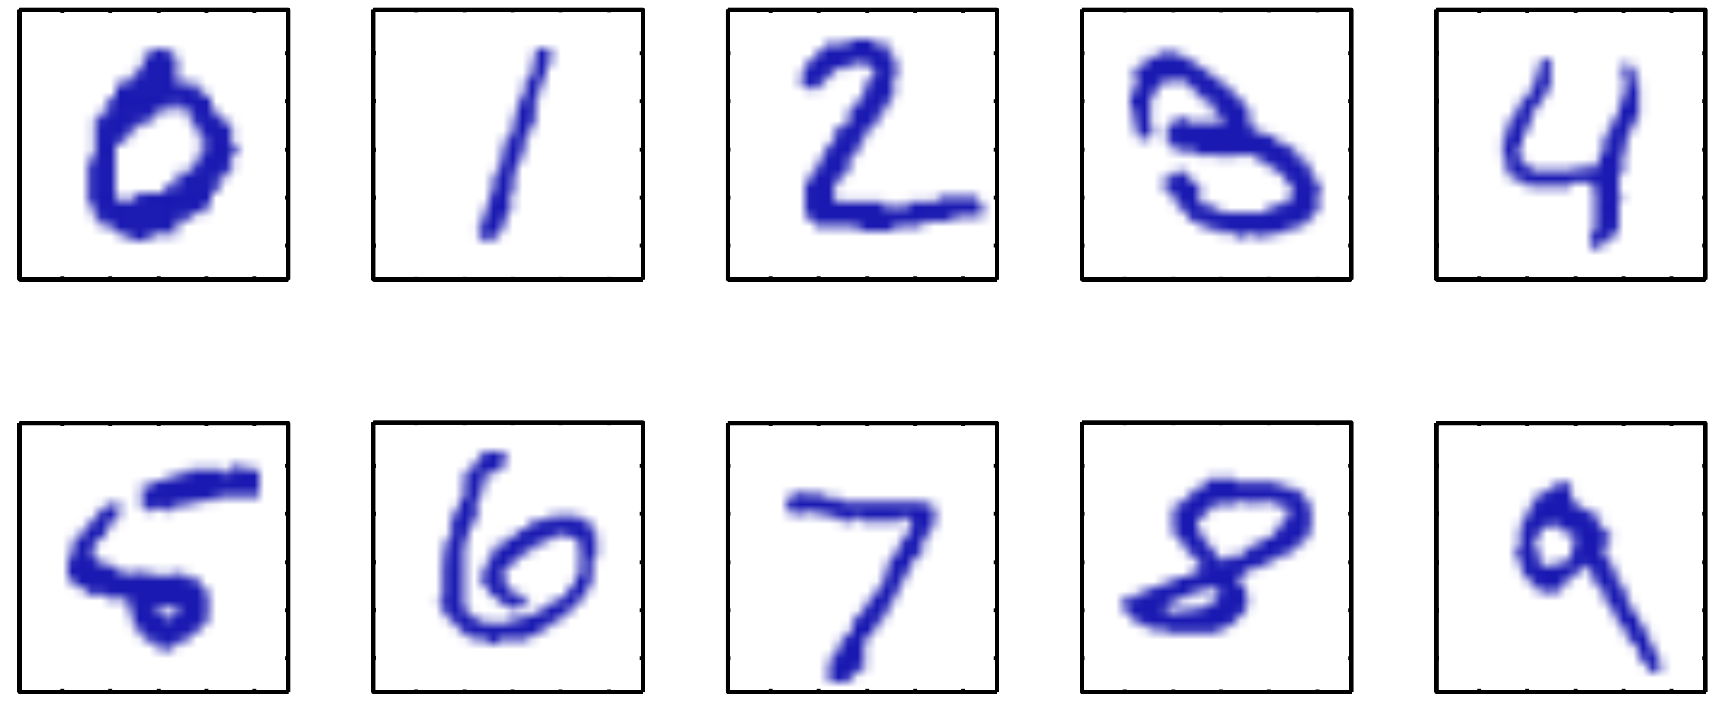
\includegraphics[scale=0.2]{chapter006/figures/fig001}
    \caption{handwritten digits}
    \label{handwritten digits}
\end{figure}

Each digit correspond to a $28 \times 28$ pixel image and so can be represented by a vector $x$ comprising $784$ real numbers. The goal is to build a machine that will take such a vector $x$ as input and that will produce the identity of the digit $0, ..., 9$ as the output.

In machine learning approach, given a large set of $N$ digits $\{x_1, ..., x_N\}$ called a \textit{training set} is used to tune the parameters of an adaptive model.

The categories of the digits in the training set are known in advance, typically by inspecting them individually and hand-labelling them.

We can express the category of a digit using \textit{target vector} $t$, which represents the identity of the corresponding digit. Note that there is one such target vector $t$ for each digit image $x$.

The result of running the machine algorithm can be expressed as a function $y(x)$ which takes a new digit image $x$ as input and that generates an output vector $y$, encoded in the same way as the target vectors.

The precise form of the function $y(x)$ is determined during the \textit{training phase}, also know as \textit{learning} phase, on the basic of the training data.

Once the model is trained it can then determine the identity of new digit images, which are said to comprise a \textit{test set}.

The ability to categorize new examples that differ from those used for training is known as \textit{generalization}.

For most practical applications, the original input variables are typically \textit{preprocessed} to transform them into some new space of variables where it is hoped, the pattern recognition problem will be easier to solve.

This pre-processing stage is sometimes also called \textit{feature extraction}. Note that new test data must be pre-processed using the same steps as the training data.

Pre-processing might also be performed in order to speed up computation or \textit{dimensionality reduction}.

Applications in which the training data comprises examples of the input vectors along with their corresponding target vectors are known as \textit{supervised learning} problems.

Assign each input vector to one of a finite number of \textbf{discrete categories}, are called \textit{classification}.

If the desired output consists of one or more continuous variables, then the task is called \textit{regression}.

\section{Polynomial Curve Fitting}

Suppose we observe a real-value input variable $x$ and we wish to use this observation to predict the value of a real-valued target variable $t$.

The data for this example is generated from the function $sin(2 \pi x)$ with random noise included in the target values.

Suppose that we are given a training set comprising $N$ observation of $x$. written $X \equiv (x_1, ..., x_N)^T$, together with corresponding observations of the values of $t$, denoted $T \equiv (t_1, ..., t_n)^T$

Our goal is to exploit this training set in order to make predictions of the value $\hat{t}$ of the target variable for some new value $\hat{x}$ of the input variables.

For the moment, we shall proceed rather informally and consider a simple approach based on curve fitting. In particular, we shall fit the data using a polynomial function of the form

\begin{equation}
    \label{Polynomial}
    y(x, \pmb{w}) = w_0 + w_1x + w_2x^2 + ... + w_Mx^M = \sum_{j=0}^Mw_jx^j
\end{equation}

where $M$ is the \textit{order} of the polynomial, and $x^j$ denotes $x$ raised to the power of $j$.

The polynomial coefficients $w_0, ..., w_M$ are collectively denoted by the vector $\pmb{w}$.

Note that, although the polynomial function $y(x, \pmb{w})$ is a nonlinear function of $x$, it is a linear function of the coefficients $\pmb{w}$. Functions, such as the polynomial, which are linear in the unknown parameters have important properties and are called \textit{linear models}.

The values of the coefficients will be determined by fitting the polynomial to the training data. This can be done by minimizing an \textit{error function} that measures the misfit between the function $y(x, \pmb{w})$, for any given value of $\pmb{w}$, and the training set data points.

One simple choice of error function, which is widely used, is given by the sum of the squares of the errors between the predictions $y(x_n, \pmb{w})$ for each data point $x_n$ and the corresponding target values $t_n$, so that we minimize

\section{Loss function}
\begin{equation}
    \label{Loss function}
    E(\pmb{w}) = \frac{1}{2} \sum_{n=1}^N \{y(x_n, \pmb{w})) - t_n \}^2
\end{equation}

where the factor of $\frac{1}{2}$ is included for later convenience.

We can solve the cure fitting problem by choosing the value of $\pmb{w}$ for which $E(\pmb{w})$ is as small as possible. Because the error function is a quadratic function of the coefficients $\pmb{w}$, its derivatives with respect to the coefficients will be linear in the elements of $\pmb{w}$, and so the minimization of the error function has a unique solution, denoted by $\pmb{w}*$, which can be found in closed form. The resulting polynomial is given by the function $y(x, \pmb{w}*)$.

There remains the problem of choosing the order $M$ of the polynomial.

We notice that the constant $(M = 0)$ and first order $(M = 1)$ polynomials give rather poor fits to the data and consequently rather poor representations of the training data.

The third order$(M = 3)$ polynomial seems to give the best fit to the data. When we go to a much higher order polynomial $(M = 9)$, we obtain an excellent fit to the training data. In fact, the polynomial passes exactly through each data point and $E(\pmb{w*}) = 0$. However, the fitted curve oscillates wildly and gives a very poor representation of the function $sin(2 \pi x)$. This latter behavior is known as \textbf{over-fitting}.




As we have noted earlier, the goal is to achieve good generalization by making accurate predictions for new data. We can obtain some quantitative insight into the dependence of the generalization performance on $M$ by considering a separate test comprising 100 data points generated using exactly the same procedure used to generate the training set points but with new choices for the random noise values included in the target values. For each choice of $M$, we can then evaluate the residual value of $E(\pmb{w*})$ for the training data, and we can also evaluate $\pmb{w*}$ for the test data set.


\begin{figure}[h]
    \centering
    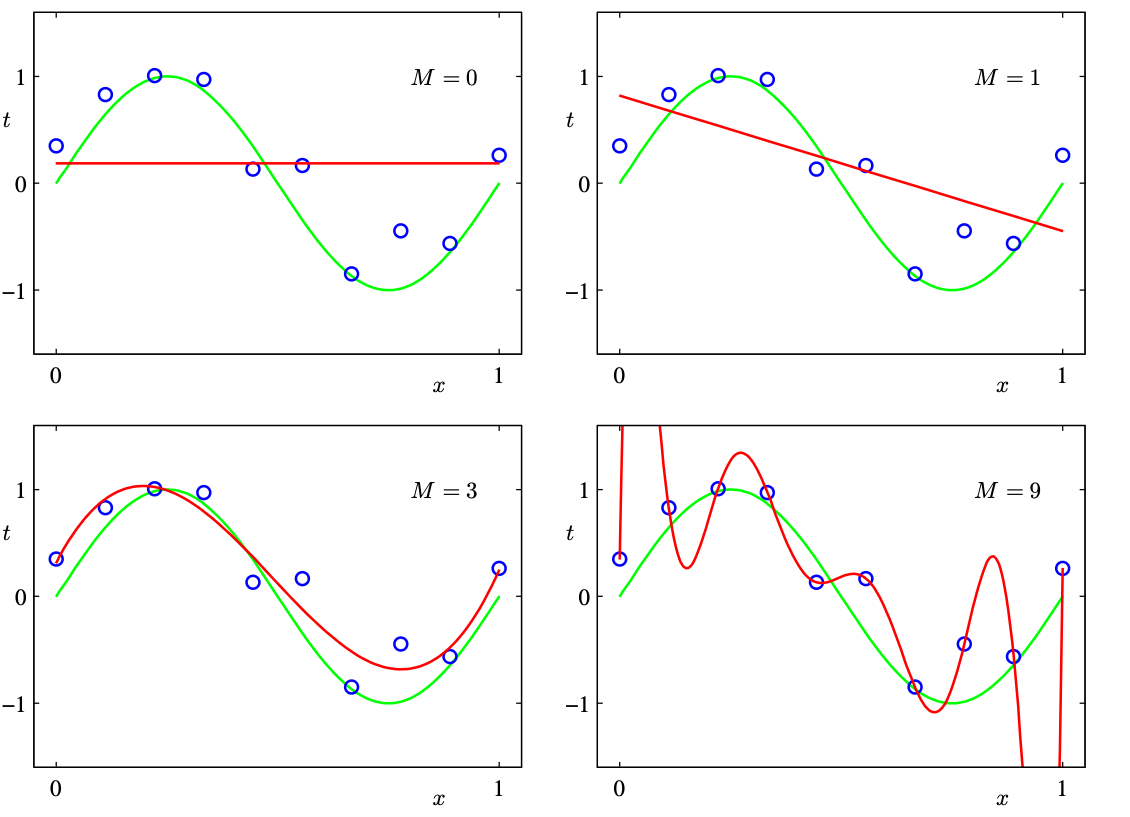
\includegraphics[scale=0.25]{chapter006/figures/fig002}
    \caption{handwritten digits}
    \label{handwritten digits}
\end{figure}

It is also interesting to examine the behavior of a given model as the size of the data set is varied. For a given model complexity, the over-fitting problem because less severe as the size of the data set increases.

It would seem more reasonable to choose the complexity of the model according to the complexity of the problem being solved.

\section{Regularization}

One technique that is often used to control the over-fitting phenomenon in such cases is that of $regularization$, which is involves adding a penalty term to the error function in order to discourage the coefficients from reaching large values.

\begin{equation}
    \tilde{E}(\pmb{w}) = \frac{1}{2}\sum_{n=1}^M \{y(x_n, \pmb{w}) - t_n \}^2 + \frac{\lambda}{2}||\pmb{w}||^2
\end{equation}

where $||\pmb{w}||^2 = \pmb{w}^T\pmb{w} = w_0^2 + w_1^2 + ... + w_M^2$, and the coefficient $\lambda$ governs the relative importance of the regularization term compared with the sum-of-squares error term. Reduces the value of the coefficients. In the context of neural networks, this approach is known as \textbf{weight decay}.

\section{Exercises}

\subsection{Exercise 1}

Consider the sum-of-squares error function given by \ref{Loss function} in which the function  $y(x, \pmb{w})$\ref{Polynomial}. Show that the coefficients $w=\{w_i\}$ that minimize this error function are given by the solution to the following set of linear equations

\begin{equation}
    \sum_{j=0}^M A_{ij}w_j = T_i
\end{equation}

where

\begin{equation}
    A_{ij} = \sum_{n=1}^N (x_n)^{i + j}
\end{equation}

and

\begin{equation}
    T_i = \sum_{n=1}^N (x_n)^it_n
\end{equation}

Here a suffix $i$ and $j$ denotes the index of a component, whereas $(x)^i$ denotes x raised to the power of $i$.

\subsubsection{Solution}

Loss function is

\begin{equation}
    E(\pmb{w}) = \frac{1}{2} \sum_{n=1}^M \{y(x_n, \pmb{w}) - t_n\}^2
\end{equation}

\begin{equation}
    \frac{\partial E(\pmb{w})}{\partial w_i} = \frac{\partial \sum_{n=1}^M \{y(x_n, \pmb{w}) - t_n\}}{\partial w_i} = \sum_{n=1}^M \frac{\partial \{y(x_n, \pmb{w}) - t_n \}}{\partial w_i}
\end{equation}

since,

\begin{equation}
    \frac{\partial \{y(x_n, \pmb{w}) - t_n \}}{\partial w_i} = \frac{\partial (w_0x_n^0 + ... + x_ix_n^i + ... + w_M x_n^M)}{\partial w_i} = x_n^i
\end{equation}

thus,


\begin{equation}
    \frac{\partial E(\pmb{w})}{\partial w_i} = \sum_{n=1}^M \{y(x_n, \pmb{w}) - t_n\} x_n^i
\end{equation}

\begin{equation}
    \frac{\partial E(\pmb{w})}{\partial w_i} = 0 \Leftrightarrow \sum_{n=1}^N \{y(x_n, \pmb{w}) - t_n\}x_n^i = 0 \Leftrightarrow \sum_{n=1}^N \{y(x_n, \pmb{w})x_n^i = \sum_{n=1}^N t_n x_n^i
\end{equation}

\begin{equation}
    \sum_{n=1}^N \{y(x_n, \pmb{w})x_n^i = \sum_{n=1}^N t_n x_n^i \Leftrightarrow \sum_{n=1}^N (\sum_{j=0}^M w_jx_n^j) x_n^i = \sum_{n=1}^N t_n x_n^i
\end{equation}

\begin{equation}
    \sum_{n=1}^N (\sum_{j=0}^M w_jx_n^j) x_n^i = \sum_{n=1}^N t_n x_n^i \Leftrightarrow \sum_{j=0}^M \sum_{n=1}^N (x_n^{(i + j)}w_j) = \sum_{n=1}^N t_nx_n^i
\end{equation}

Intuitively, given N = 2, M = 2

\begin{equation}
    \begin{split}
        \sum_{n=1}^N \sum_{j=0}^M (w_jx_n^i)x_n^i & = \sum_{n=1}^N (w_0x_n^0 + w_1x_n^1 + w_2x_n^2)x_n^i\\
        & = \sum_{n=1}^N (w_0x_n^0x_n^i + w_1x_n^1x_n^i + w_2x_n^2x_n^i)\\
        & = (w_0x_1^1x_1^i + w_1x_1^1x_1^i + w_2x_1^2x_1^i) + (w_0x_2^1x_2^i + w_1x_2^1x_2^i + w_2x_2^2x_2^i)\\
        & = \sum_{j=0}^M (w_jx_1^jx_1^i) + \sum_{j=0}^M (w_jx_2^jx_2^i)\\
        & = \sum_{j=0}^M (w_jx_1^{(i+j)}) + \sum_{j=0}^M (w_jx_2^{(i+j)})\\
        & = \sum_{j=0}^M \sum_{n=1}^N x_i^{(i + j)}w_j
    \end{split}    
\end{equation}


If $A_{ij} = \sum_{n=1}^N x_n^{(i + j)}$ and $T_i = \sum_{n=1}^N x_n^it_n$, then

\begin{equation}
    \sum_{j=0}^M A_{ij}w_j = T_i
\end{equation}


\subsection{Exercise 2}

Similar to the exercise 1, but now apply to the loss function

\begin{equation}
    E(\pmb{w}) = \frac{1}{2} \sum_{n=1}^M \{y(x_n, \pmb{w}) - t_n\}^2 +  \frac{\lambda}{2} ||w_i||^2
\end{equation}

since $||w_i||^2 = w_i^2 $, we have

\begin{equation}
    \frac{\partial E(\pmb{w})}{\partial w_i} = \sum_{n=1}^N \{y(x_n, \pmb{w}) - t_n\} x_n^i + \lambda w_i = \sum_{n=1}^N \{y(x_n, \pmb{w})x_n^i - \sum_{n=1}^N t_nx_n^i + \lambda w_i
\end{equation}

\begin{equation}
    \frac{\partial E(\pmb{w})}{\partial w_i} = 0 \Leftrightarrow \sum_{n=1}^N \{y(x_n, \pmb{w})x_n^i + \lambda w_i = \sum_{n=1}^N t_n x_n^i 
\end{equation}


\begin{equation}
    \frac{\partial E(\pmb{w})}{\partial w_i} = 0 \Leftrightarrow \sum_{j=0}^M (\sum_{n=1}^N x_n^{(i + j)}w_j) + \lambda w_i = \sum_{n=1}^N t_n x_n^i 
\end{equation}

Intuitively, given $M = 2$ and $N = 2$, then $\sum_{j=0}^M \sum_{n=1}^N (x_n^{(i + j)})w_j + \lambda w_i$ equals

\begin{equation}
    \begin{split}
        & = \sum_{j=0}^M (x_1^{(i + j)} + x_2^{(i + j)})w_j + \lambda w_i\\
        & = (x_1^{(i + j)} + x_2^{(i + j)})w_0 + (x_1^{(i + j)} + x_2^{(i + j)})w_1 + (x_1^{(i + j)} + x_2^{(i + j)})w_2 + \lambda w_i
    \end{split}
\end{equation}

since $0 \leq i \leq M$, if $i=1$, then 

\begin{equation}
    \begin{split}
        & = (x_1^{(i + j)} + x_2^{(i + j)})w_0 + (x_1^{(i + j)} + x_2^{(i + j)})w_1 + (x_1^{(i + j)} + x_2^{(i + j)})w_2 + \lambda w_1\\
        & = (x_1^{(i + j)} + x_2^{(i + j)})w_0 + (x_1^{(i + j)} + x_2^{(i + j)} + \lambda)w_1 + (x_1^{(i + j)} + x_2^{(i + j)})w_2\\
        & = (x_1^{(i + j)} + x_2^{(i + j)} + \delta \lambda)w_0 + (x_1^{(i + j)} + x_2^{(i + j)} + \delta \lambda)w_1 + (x_1^{(i + j)} + x_2^{(i + j)} + \delta \lambda)w_2
    \end{split}
\end{equation}

where $\delta = 0$ if $i \neq j$, otherwise $\delta = 1$. So

 \begin{equation}
     \begin{split}
         \sum_{j=0}^M (\sum_{n=1}^N x_n^{(i + j)}w_j) + \lambda w_i = \sum_{j=0}^M (\sum_{n=1}^N x_n^{(i + j)}w_j + \delta \lambda)
     \end{split}
 \end{equation}
 
 or
 
 \begin{equation}
     \frac{\partial E(\pmb{w})}{\partial w_i} = 0 \Leftrightarrow \sum_{j=0}^M (\sum_{n=1}^N x_n^{(i + j)}w_j + \delta \lambda) = \sum_{n=1}^N t_n x_n^i
 \end{equation}
\chapter{Linear Models for Regression}

\section{Linear Basis Function Models}

Given a training data set comprising $N$ observations $\{x_n\}$, where $n=1, ..., N$, together with corresponding target values $\{t_n\}$, the goal is to predict the value of $t$ for a new value of $x$. In the simplest approach, this can be done by directly constructing an appropriate function $y(x)$ whose values for new inputs $x$ constitue the predictions for the corresponding values of $t$.

The simplest linear model for regression is one that involves a linear combination of the input variables

\begin{equation}
    y(x, \pmb{w}) = w_0 + w_1x_1 + ... + w_Dx_D
\end{equation}

where $x = (x_1, ..., x_D)^T$. This is often simply known as \textbf{linear regression}. It is also a linear function of the input variables $x_i$, and this imposes significant limitations on the model. We therefore extend the class of models by considering linear combinations of fixed nonlinear functions of the input variables, of the form

\begin{equation}
    y(x, \pmb{w}) = w_0 + \sum_{j=1}^{M - 1}w_j \phi_j (x)
\end{equation}

where $\phi_j(x)$ are known as \textbf{basic functions}. By denoting the maximum value of the index $j$ by $M - 1$, the total number of parameters in this model will be $M$.

The parameter $w_0$ allows for any fixed offset in the data and is sometimes called a bias parameter (not to be confused with " bias" in a statistical sense).

It is often convenient to define an additional dummy "basic function" $\phi_0 (x) = 1$ so that

\begin{equation}
    y(x, \pmb{w}) = \sum_{j=1}^{M - 1}w_j \phi_j (x) = \pmb{w}^T \phi (x)
\end{equation}

where $\pmb{w} = (w_0, ..., w_{M - 1})^T$ and $\phi = (\phi_0, ..., \phi _{M - 1})^T$.

For example $\phi_j(x) = x^j$. One limitation of polynomial basic functions is that they are global functions of the input variable, so that changes in one region of input space affect all other regions.

In many practical applications of pattern recognition, we will apply some form of fixed pre-processing, of feature extraction, to the original data variables.

If the original variables comprise the vector $x$, then the features can be expressed in terms of the basis functions $\{\phi_j (x)\}$.

\textbf{By using nonlinear basis functions}, we allow the function $y(x, \pmb{w})$ to be a non-linear of the input vector $x$.

\section{Maximum likelihood and Least Squares}
we assume that the target variable $t$ is given by a deterministic function $y(x, \pmb{w})$ with additive Gaussian noise so that

\begin{equation}
    t = y(x, \pmb{w}) + \epsilon
\end{equation}

where $\epsilon$ is a zero mean Gaussian random variable with precision $\beta^{-1} = \sigma^2 \Leftrightarrow \beta = \frac{1}{\sigma^2}$, $\beta$ is maximum when $\sigma^2$ is minimum.

We assume that, given the value of $x$, the corresponding value of $t$ has a Gaussian distribution with a mean equal to the value $y(x, \pmb{w})$.

\begin{equation}
    p(t|x, \pmb{w}, \beta) = \mathcal{N}(t | y(x, \pmb{w}), \beta^{-1})
\end{equation}

If we assume a squared loss function, then the optimal prediction, for a new value of $x$, will be given by the conditional mean of the target variable.

\begin{equation}
    \mathbb{E}[t|x] = \int tp(t|x)dt = y(x, \pmb{w}) 
\end{equation}

Now consider a data set of inputs $X = \{x_1, ..., x_N\}$ with corresponding target values $t_1, ..., t_N$. We group the target variables $\{t_n\}$ into a column vector that we denote by $\pmb{t}$.

Making the assumption that these data points are drawn independently from the distribution

\begin{equation}
    \mathbb{E}[t|x] = \int tp(t|x)dt = y(x, \pmb{w}) 
\end{equation}

we obtain

\begin{equation}
    p(\pmb{t} | \pmb{X}, \pmb{w}, \beta) = \prod_{n=1}^N \mathcal{N}(t_n | \pmb{w}^T \phi(x_n), \beta^{-1})
\end{equation}

Note that in supervised learning problems, we are not seeking to model the distribution of the input variables. Thus $x$ will always appear in the set of conditioning variables, and so from now on we will drop the explicit $x$ from expressions such as $p(\pmb{t}|x, \pmb{w}, \beta)$ in order to keep the notation uncluttered.

\begin{equation}
    \begin{split}
        ln (p(\pmb{t} | \pmb{w}, \beta)) & = \sum_{n=1}^N ln \mathcal{N}(t_n| \pmb{w}^T \phi(x_n), \beta^{-1})\\
        & = \sum_{n=1}^N ln [ \frac{1}{(2\pi \sigma^2)^{1/2}} exp \{ - \frac{1}{2\sigma^2} (t_n - \pmb{w}^T \phi (x_n))^2\}]\\
        & = \sum_{n=1}^N ln [ \frac{1}{(2\pi \sigma^2)^{1/2}}] + \sum_{n=1}^N ln[exp \{ - \frac{1}{2\sigma^2} (t_n - \pmb{w}^T \phi (x_n))^2\}]]\\
        & = \sum_{n=1}^N ln (1) - \sum_{n=1}^N ln(2\pi \sigma^2)^{1/2}) - \sum_{n=1}^N \frac{1}{2\sigma^2} (t_n - \pmb{w}^T \phi (x_n))^2\\
        & = - \frac{1}{2}\sum_{n=1}^N ln(2\pi \sigma^2) - \sum_{n=1}^N \frac{1}{2\sigma^2} (t_n - \pmb{w}^T \phi (x_n))^2\\
        & = - \frac{1}{2}\sum_{n=1}^N ln(2\pi) - \frac{1}{2}\sum_{n=1}^N ln(\sigma^2) - \sum_{n=1}^N \frac{1}{2\sigma^2} (t_n - \pmb{w}^T \phi (x_n))^2\\
        & = - \frac{1}{2}\sum_{n=1}^N ln(2\pi) + \frac{1}{2}\sum_{n=1}^N ln(\sigma^{-2}) - \frac{1}{2\sigma^2}\sum_{n=1}^N (t_n - \pmb{w}^T \phi (x_n))^2\\
        & = - \frac{1}{2}\sum_{n=1}^N ln(2\pi) + \frac{1}{2}\sum_{n=1}^N ln(\frac{1}{\sigma^{2}}) - \frac{1}{2\sigma^2}\sum_{n=1}^N (t_n - \pmb{w}^T \phi (x_n))^2\\
        & = - \frac{1}{2}\sum_{n=1}^N ln(2\pi) + \frac{1}{2}\sum_{n=1}^N ln(\beta) - \beta\frac{1}{2}\sum_{n=1}^N (t_n - \pmb{w}^T \phi (x_n))^2\\
    \end{split}
\end{equation}

Let the sum-of-squares error function is defined by

\begin{equation}
    E_D(w) = \frac{1}{2}\sum_{n=1}^N (t_n - w^T \phi (x_n))^2
\end{equation}

\textbf{Maximization of the likelihood function under a conditional Gaussian noise distribution for a linear model is equivalent to minimizing a sum-of-squares error function given by} $E_D(\pmb{w})$. The gradient of the log likelihood function takes the form

\begin{align}
    \begin{split}
        \nabla ln (p(\pmb{t} | \pmb{w}, \beta)) & = 
    \end{split}
\end{align}

\chapter{Lagrange Multipliers}

\section{Method of Lagrange Multipliers}

\begin{theorem}
    To find the maximum and minimum values of $f(x, y, z)$ subject to the constraint $g(x, y, z) = k$ [assuming that these extreme values exist and $\nabla g \neq 0$ on the surface $g(x, y, z)=k$]:
    \begin{enumerate}
        \item Find all values of $x, y, z$ and $ \lambda $ such that
            \begin{equation}
                \label{eq: Lagrange Multipliers}
                \nabla f(x, y, z) = \lambda \nabla g(x, y, z)
            \end{equation}
            and
            \begin{equation}
                \label{eq: Lagrange Multipliers}
                \nabla g(x, y, z) = k
            \end{equation}
        \item Evaluate $f$ at all the points $(x, y, z)$ that result from step 1. The largest of these values is the maximum value of $f$; the smallest is the minimum value of $f$.
    \end{enumerate}
\end{theorem}

\begin{flushleft}
    If we write the vector equation $\nabla f = \lambda \nabla g$ in terms of components, then the equations in step 1 become
    \begin{equation}
        \label{eq: Lagrange Multipliers}
        f_x = \lambda g_x \ \ \ f_y=\lambda g_y \ \ \ f_z=\lambda g_z \ \ \ g(x, y, z) = k
    \end{equation}
\end{flushleft}

\begin{flushleft}
    This is a system of four equations in the four unknowns $x, y, z$ and $\lambda$, and we must find all possible solutions (although the explicit values of $\lambda$ are not needed for the conclusion of the method).
\end{flushleft}

\begin{flushleft}
    Given $x=x_0, y=y_0, z=z_0$ is a solution to this system of equations, we have
    
    \begin{enumerate}
        \item if the value of $\lambda$ is 0, then $\nabla f(x_0, y_0, z_0)=0$ and so  $(x_0, y_0, z_0)$ is a critical point of $f$.
        \item if $\lambda$ is not 0, then $\lambda f(x_0, y_0, z_0)$ and $\lambda f(x_0, y_0, z_0)$ are parallel.
        \end{enumerate}
\end{flushleft}

\subsection{Example 1}

Find the extreme values of the function $ f(x, y)=x^2 + 2y^2 $ on the circle $ x^2 + y^2=1 $

\begin{figure}
    \centering
    \subfloat
        \centering
        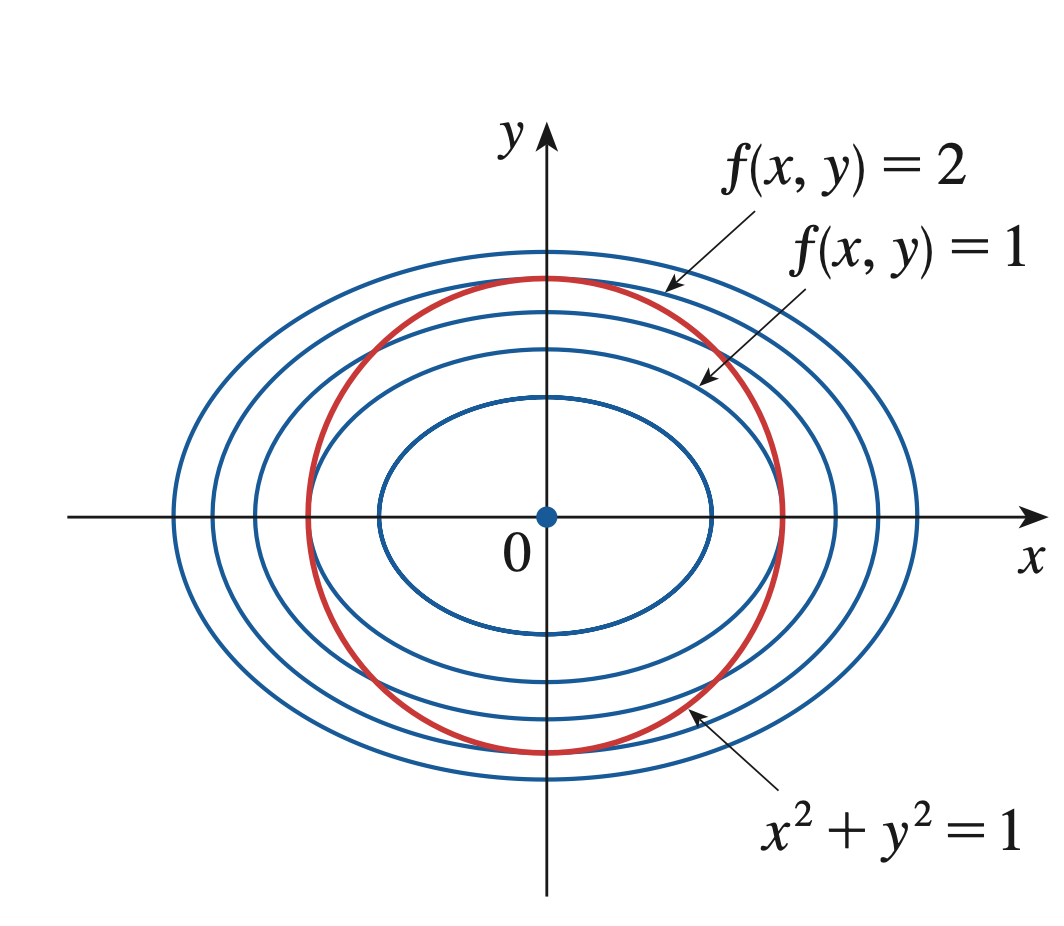
\includegraphics[width=5cm]{chapter003/figures/fig002}
    \qquad
    \subfloat
        \centering
            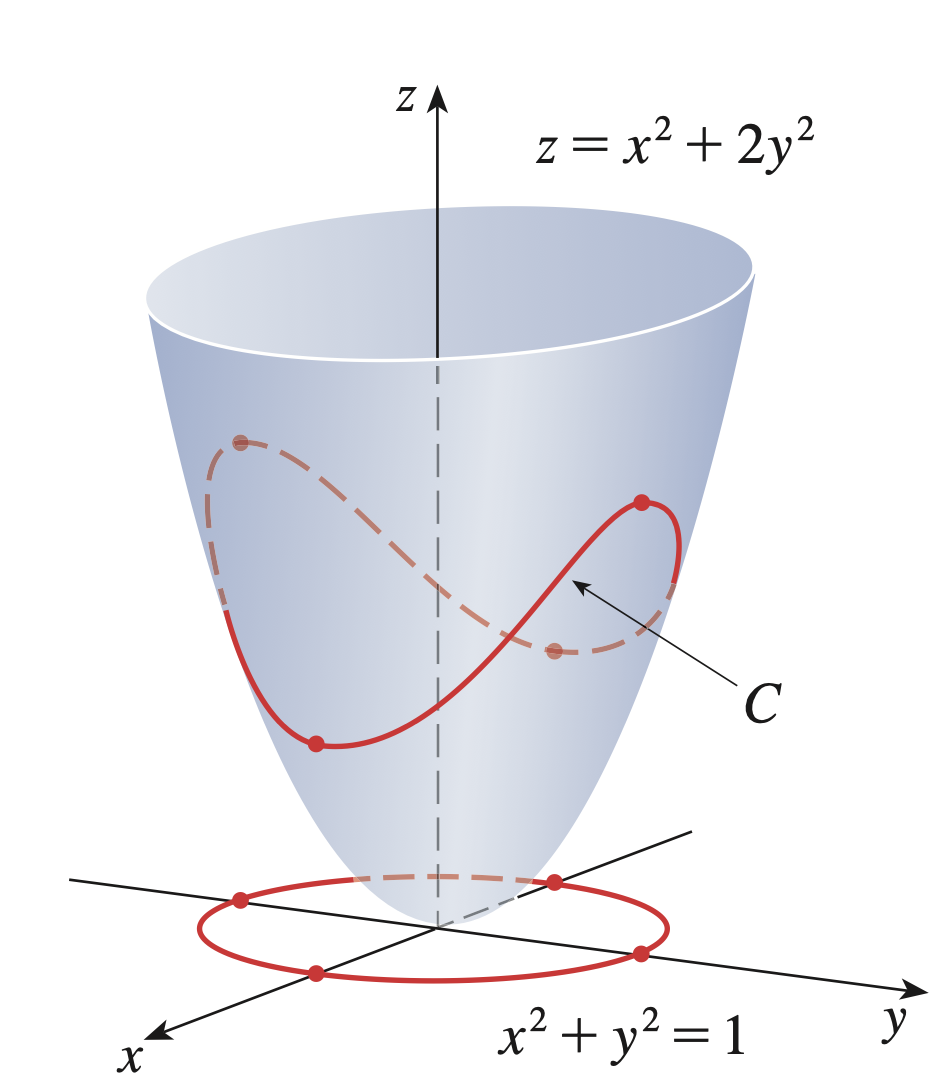
\includegraphics[width=5cm]{chapter003/figures/fig001}
    \label{fig:example}
\end{figure}

\subsubsection{Solution}
We are asked for the extreme values of $f$ subject to the constraint $g(x, y)=x^2 + y^2=1$. Using Lagrange multipliers, we solve the equations $g(x, y)=x^2 + y^2=1$. Using Lagrange multipliers, we solve the equations $\nabla f = \lambda \nabla g$ and $g(x, y)=1$, which can be written as
\begin{equation}
    f_x = \lambda g_x \ \ \ f_y = \lambda g_y \ \ \ g(x, y)=1
\end{equation}
where
\begin{equation}
    f_y = 2x \ \ \ f_y = 4y \ \ \ g_x = 2x \ \ \ g_y = 2y
\end{equation}
then,
\begin{equation}
    2x = \lambda 2x \ \ \ 4y = \lambda 2y \ \ \ x^2 + y^2 = 1
\end{equation}
thus,

\begin{equation}
    2x(1 - \lambda) = 0 \Leftrightarrow
  \left\{
    \begin{aligned}
      & \lambda = 1 \Leftrightarrow y = 0 \Leftrightarrow x= \pm 1\\
      & x = 0 \Leftrightarrow y = \pm 1\ (x^2 + y^2=1)
    \end{aligned}
  \right.
\end{equation}

Therefore, $f$ has possible extreme values at the points $(0, 1), (0, -1)$ and $(1, 0)$ and $(-1, 0)$. Evaluating $f$ at these four points, we find that
\begin{equation}
    f(0, 1) = 2 \ \ \ f(0, -1) = 2 \ \ \ f(1, 0) = 1 \ \ \ f(-1, 0) = 1
\end{equation}
thus, the maximum value of $f$ on the circle $x^2 + y^2=1$ is $f(0, \pm 1)=2$ and the minimum value is $f(\pm 1, 0)=1$

\section{Applications in Machine Learning}
Consider a $D-$dimensional variable \textbf{$x$} with components $x_1, ..., x_D$.

\begin{align}
    x &= \begin{bmatrix}
           x_{1} \\
           x_{2} \\
           \vdots \\
           x_{D}
         \end{bmatrix}
\end{align}

\begin{flushleft}
The constraint equation $g(x)=0$ then represents a $(D-1)$-dimensional surface in x-space. For example, 3-D function $z=x^2+y^2$ and 2-D function $1=x^2+y^2$ are represented in the following figure. In the latter function, $z$ is now a constant.
\end{flushleft}

\begin{figure}
    \centering
    \subfloat
        \centering
        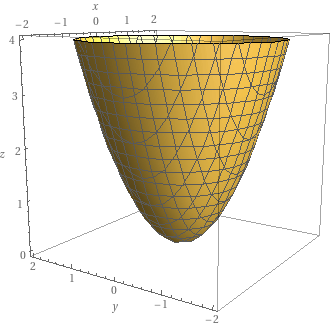
\includegraphics[width=5cm]{chapter003/figures/fig003}
    \qquad
    \subfloat
        \centering
            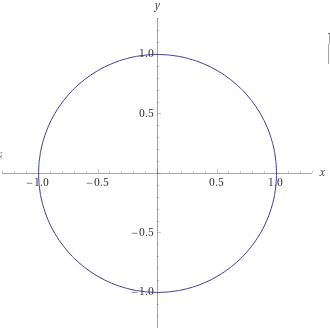
\includegraphics[width=5cm]{chapter003/figures/fig004}
    \label{fig:example}
\end{figure}

According to the equation \ref{eq: Lagrange Multipliers}, we have

\begin{equation}
    \nabla f = \lambda \nabla g \Leftrightarrow \nabla f + \lambda \nabla g = 0
\end{equation}
where $\lambda \neq 0$ is known as a Lagrange multiplier. Note that $\lambda$ can have either sign.

\subsection{Lagrangian function}
\begin{equation}
    \label{eq: Lagrangian function}
    L(x, \lambda) \equiv f(x) + \lambda g(x)
\end{equation}

\begin{flushleft}
Since $\partial L / \partial \lambda = g(x)$, the condition $\partial L / \partial \lambda = 0$ leads to the constraint equation $g(x)=0$.

To find the maximum of a function $f(x)$ subject to the constraint $g(x)=0$, we define the \ref{eq: Lagrangian function} and then find the stationary point of $L(x, \lambda)$ with respect to both $x$ and $\lambda$.
\end{flushleft}

For a $D-$dimensional vector $x$, this gives $D+1$ equations that determine both the stationary point $x*$ and the value $\lambda$. (Why $D+1$ equations? $D$-equations from $x$ and $g(x)=0$)

If we are only interested in $x*$, then we can eliminate $\lambda$ from the stationarity equations without needing to find its value.

As a simple example, suppose we wish to find the stationary point of the function $f(x_1. x_2)=1 - x_1^2 - x_2^2$ subject to the constraint $g(x_1, x_2)=x_1 + x_2 -1 = 0$. The corresponding Lagrangian function is given by 
\begin{equation}
    L(x, \lambda) = 1 - x_1^2 - x_2^2 + \lambda (x_1 + x_2 - 1) = 1 - x_1^2 - x_2^2 + \lambda x_1 + \lambda x_2 - \lambda
\end{equation}

The conditions for this Lagrangian to be stationary with respect to $x_1$, $x_2$ and $\lambda$ give the following coupled equations:

 
\begin{equation}
  \left\{
    \begin{aligned}
      & \frac{\partial L}{\partial x_1} = -2x_1 + \lambda\\
      & \frac{\partial L}{\partial x_2} = -2x_2 + \lambda\\
      & x_1 + x_2 - 1= 0
    \end{aligned}
  \right.
  \Leftrightarrow
  \left\{
    \begin{aligned}
      & x_1 = \frac{1}{2}\\
      & x_2 = \frac{1}{2}\\
      & \lambda = 1
    \end{aligned}
  \right.
\end{equation}

Solution of these equations then gives the stationary point as $(x_1*, x_2*)=(\frac{1}{2}, \frac{1}{2})$ and $\lambda = 1$.







\chapter{Principal Component Analysis}
\section{Maximum variance formulation}

\begin{itemize}
    \item A dataset of observations $\{X_n\}$ where $n = 1, ..., N$, and $X_n$ is a Euclidean variable with dimensionality $D$.
    \item Projecting the data onto a space having dimensionality $M<D$ \textbf{while maximizing the variance} of the projected data
\end{itemize}
 
 \begin{flushleft}
 Consider the projection onto a one-dimensional space ($M=1$).
 Defining the direction of this space using a $D-dimensional$ vector $u_1$ such that $u_1^Tu_1=1$ (unit vector)
 \end{flushleft}

\begin{equation}
    \label{eq:PCA_mean_vector}
    \overline{x} = \frac{1}{N}\sum_{n=1}^{N} x_n
\end{equation}

and the variance of the projected data is given by

\begin{equation}
    \label{eq:PCA_variance}
    \frac{1}{N}\sum_{n=1}^{N} \{u_1^Tx_n - u_1^T \overline{x}\}^2=u_1^TSu_1
\end{equation}

where $S$ is the data covariance matrix defined by

\begin{equation}
    \label{eq:PCA_covariance_matrix}
    \frac{1}{N}\sum_{n=1}^{N} \{u_1^Tx_n - u_1^T \overline{x}\}^2=u_1^TSu_1
\end{equation}

\subsubsection{Proof}
\begin{equation}
    \label{eq:PCA_covariance_proof}
    \frac{1}{N}\sum_{n=1}^{N} \{u_1^Tx_n - u_1^T \overline{x}\}^2=\frac{1}{N}\sum_{n=1}^{N}\{u_1^T(x_n - \overline{x})\}^2=\frac{1}{N}\sum_{n=1}^{N}\{u_1^T(x_n - \overline{x})u_1^T(x_n - \overline{x})\}
\end{equation}
\begin{equation}
    \label{eq:PCA_covariance_proof}
    \frac{1}{N}\sum_{n=1}^{N}\{u_1^T(x_n - \overline{x})u_1^T(x_n - \overline{x})\}=\frac{1}{N}\sum_{n=1}^{N}\{u_1^T(x_n - \overline{x})(x_n - \overline{x})^Tu_1\}=u_1^T\frac{1}{N}\sum_{n=1}^{N}\{(x_n - \overline{x})(x_n - \overline{x})^T\}u_1
\end{equation}

We now maximize the projected variance $u_1^TSu_1$ with respect to $u_1$. Clearly, this has to be a constrained maximization to prevent $||u_1|| \rightarrow \infty$. The appropriate constraint comes from the normalization condition $u_1^Tu_1=1$. To enforce this constraint, we introduce a Lagrange multiplier that we shall denote by $\lambda_1$, and then make an unconstrained maximization of

\begin{equation}
    \label{eq:PCA_optimize}
    L = u_1^TSu_1 + \lambda_1(1 - u_1^Tu_1)
\end{equation}

where $f(x)=u_1^TSu_1$ and $g(x)=1 - u_1^Tu_1$ and the equation \ref{eq: Lagrangian function}.

By setting the derivative with respect to $u_1$ equal to zero, we see that this quantity will have a stationary point when

\begin{equation}
    \label{eq:PCA_stationary_point}
    Su_1 = \lambda_1u_1
\end{equation}

which says that $u_1$ must be an eigenvector of $S$.

\subsubsection{Proof}
\begin{equation}
    \frac{\partial L}{\partial u_1}=u_1^TS - \lambda_1u_1^T
\end{equation}

$$\frac{\partial L}{\partial u_1} = 0 \Leftrightarrow (u_1^TS - \lambda_1u_1^T)=0 \Leftrightarrow u_1^TS = \lambda_1u_1^T \Leftrightarrow Su_1=\lambda u_1$$

If we left-multiply by $u_1^T$ and make use of $u_1^Tu_1=1$, we see that the variance is given by $$u_1^TSu_1=\lambda_1$$. Because $$Su_1=\lambda u_1 \Leftrightarrow u_1^TSu_1=u_1^T\lambda u_1 \Leftrightarrow u_1^TSu_1=\lambda_1 u_1^T u_1 \Leftrightarrow u_1^TSu_1=\lambda_1$$
Notice that the $\lambda_1$ is a constant number.

The variance will be maximum when we set $u_1$ equal to the eigenvector having the largest eigenvalue $\lambda_1$. This eigenvector is known as the first principal component.


\chapter{Support Vector Machines}

\section{Discriminant Functions}
A discriminant is a function that takes an input vector $x$ and assigns it to one of $K$ classes, denoted $C_k$
The simplest representation of a linear discriminant function is obtained by taking a linear function of the input vector so that
\begin{equation}
    \label{eq: discriminant classifier}
    y(x) = w^Tx + w_0    
\end{equation}

where $w=(w_0, ..., w_{M-1})^T$ and $x=(x_1, ..., x_D)^T$. $w$ is called a weight vector, and $w_0$ is a bias. An input vector $x$ is assigned to class $C_1$ if $y(x) \geq 0$ and to class $C_2$ otherwise. The corresponding decision boundary is therefore defined by the relation $y(x)=0$, which corresponds to a $(D-1)$

Consider two points $x_A$ and $x_B$ both of which lie on the decision surface. Because $y(x_A) = y(x_B) = 0$, we have $w^T(x_A - x_B)=w^TA - w^TB=0$ and hence the vector $w$ is orthogonal to every vector lying within the decision surface.

If $x$ is a point on the decision surface, then $y(x) = 0$, then
\begin{equation}
    y(x) = 0 \Leftrightarrow w^Tx + w_0 = 0 \Leftrightarrow w^Tx = -w_0 \Leftrightarrow \frac{w^Tx}{||w||} = - \frac{w_0}{||w||}
\end{equation}

The bias parameter $w_0$ determines the location of the decision surface.
Consider an arbitrary point $x$ and let $x_\bot$ be its orthogonal projection onto the decision surface, so that
\begin{equation}
    x = x_\bot + r \frac{w}{||w||} \Leftrightarrow w^T x = w^Tx_\bot + r w^T \frac{w}{||w||} = w^Tx_\bot + r\frac{w^2}{||w||} = w^Tx_\bot + r||w||
\end{equation}

If we add $w_0$ to both sides of the above equation, we have
\begin{equation}
    w^T + x_0 = w^Tx_\bot + w_0 + r||w|| \Leftrightarrow y(x) = r||w|| \Leftrightarrow r = \frac{y(x)}{||w||}
\end{equation}

The value of $y(x)$ gives a signed measure of the perpendicular distance $r$ of the point $x$ from the decision surface. $r$ is called \textbf{perpendicular distance}.

\begin{figure}
    \centering
    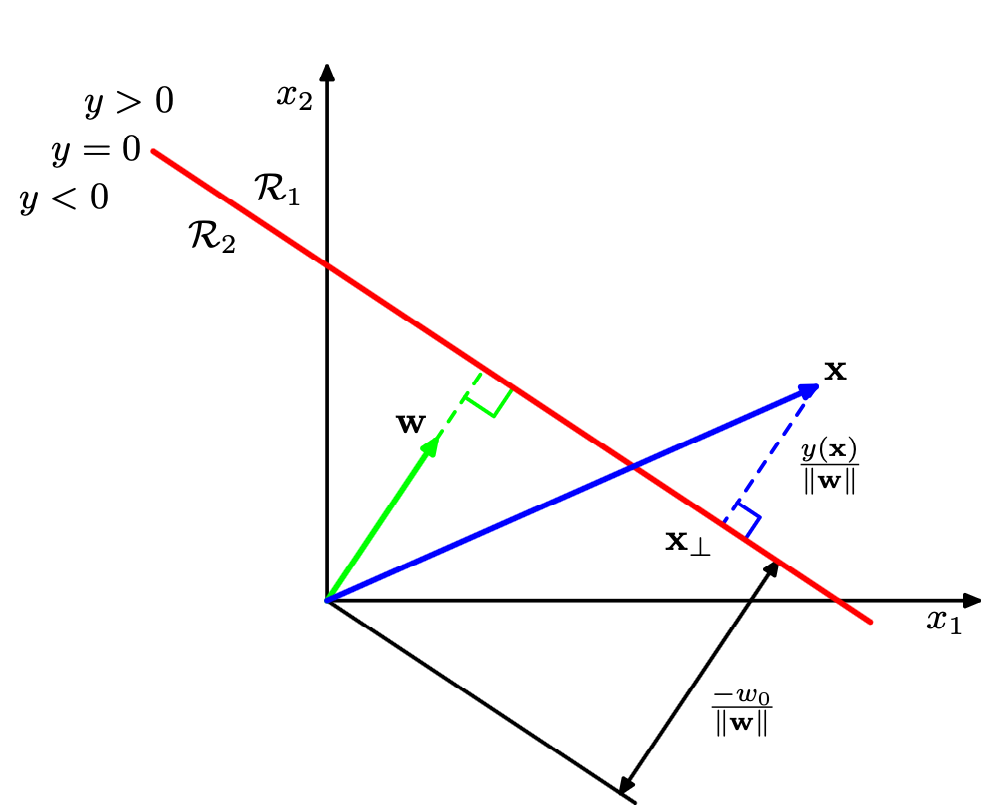
\includegraphics[scale=0.3]{chapter005/figures/fig003}
    \label{fig: geometry of a linear discriminant function}
    \caption{Illustration of the geometry of a linear discriminant function in two dimensions}
\end{figure}

\section{Maximum Margin Classifiers}

\begin{definition}
    Two-class classification problem using linear models of the form
    \begin{equation}
        \label{svm linear model}
        y(x)=w^T \phi (x) + b
    \end{equation}
    where $\phi (x)$ denotes a fixed feature-space transformation, and we have made the bias parameter $b$ explicit.
\end{definition}

The training data set comprises $N$ input vectors $x_1, ..., x_N$, with corresponding target values $t_1, ..., t_N$ where $t_n \in \{-1, 1\}$, and new data points $x$ are classified according to the sign of $y(x)$.

We shall assume for the moment that the training data set is linearly separable in feature space, so that by definition there exits at least one choice of the parameters $w$ and $b$ such that \ref{svm linear model} satisfies $y(x_n) > 0$ for points having $t_n = +1$ and $y(x_n) < 0$ for points having $t_n=-1$, so that $t_ny(x_n) > 0$ for all training data points.

The support vector machine minimize the generalization error through the concept of the $margin$, which is defined to be the smallest distance between the decision boundary and any of the samples.

\begin{figure}
    \centering
    \subfloat
        \centering
        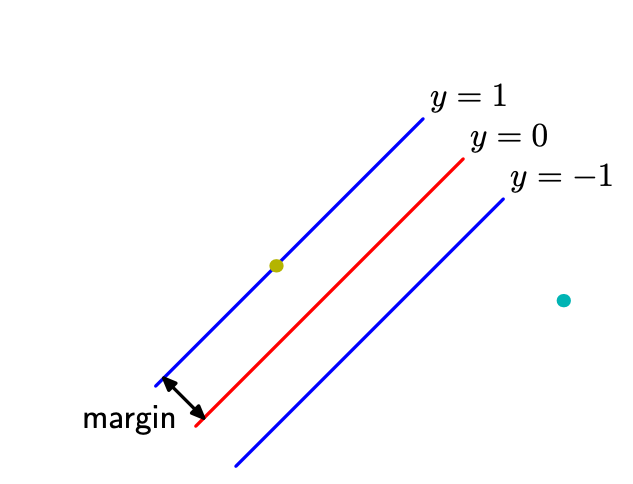
\includegraphics[width=5cm]{chapter005/figures/fig001}
    \qquad
    \subfloat
        \centering
            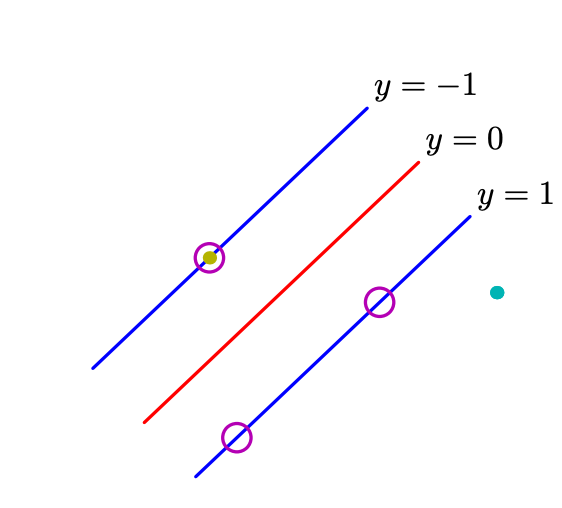
\includegraphics[width=5cm]{chapter005/figures/fig002}
    \label{fig:example}
    \caption{The margin is defined as the perpendicular distance between the decision boundary and the closest of the data points.}
\end{figure}

\textbf{In support vector machines, the decision boundary is chosen to be the one for which the margin is maximized}.

The perpendicular distance of a point $x$ from a hyperplane defined by $y(x)=0$ is given by $\frac{|y(x)|}{||w||}$.
We are only interested in solutions for which all data points are correctly classified, so that $t_ny(x_n)>0$ for all $n$.

Thus the distance of a point $x_n$ to the decision surface is given by
\begin{equation}
    \frac{t_ny(x_n)}{||w||} = \frac{t_n(w^T\phi(x_n) + b)}{||w||}
\end{equation}

The margin is given by the perpendicular distance to the closest point $x_n$ from the data set, and we wish to optimize the parameters $w$ and $b$ in order to maximum this distance. Thus the maximum margin solution is found by solving
\begin{align}
    \label{formula:SVM_optimize}
    \operatorname*{argmax}_{w,b} & \left \{ \frac{1}{||w||} \operatorname*{min}_{n}\left[ t_n(w^T\phi (x_n) + b) \right] \right \}
\end{align}

Note that if we make the rescaling $w \rightarrow kw$ and $b \rightarrow kb$, then the distance from any point $x_n$ to the decision surface, given by $t_ny(x_n)/||w||$, is unchanged.

\subsubsection{Proof}

Given $w=(w_0, ..., w_{M-1})$, then rescale $w \rightarrow kw$ means  $kw = (kw_0, ..., kw_{M-1})$, we have
\begin{equation}
    \label{eq: rescaling vector}
    \begin{split}
     ||kw|| & = \sqrt{(kw_0)^2 + (kw_1)^2 + ... + (kw_{M-1})^2} \\
            & = \sqrt{k^2(w_0^2 + w_1^2 + ... + w_{M-1}^2)} \\
            & = k||w||
     \end{split}
\end{equation}
and
\begin{equation}
       \frac{t_n((kw)^T\phi(x_n) + kb)}{||kw||}
        = \frac{kt_n((w)^T\phi(x_n) + b)}{k||w||} = \frac{t_n(w^T\phi(x_n) + b)}{||w||}
\end{equation}

We have,

\begin{equation}
    \frac{t_ny(x_n)}{||w||} = \frac{t_n(w^T\phi(x_n) + b)}{||w||} = d
\end{equation}

where $d$ is the distance from the closest data point to the hyper-plane. In other words,

\begin{equation}
    t_n(w^T\phi(x_n) + b) = d||w|| \Leftrightarrow \frac{t_n(w^T\phi(x_n) + b)}{d||w||} = 1
\end{equation}


\begin{align}
    \label{formula:SVM_optimize}
    \operatorname*{argmax}_{w,b} & \left \{ \frac{1}{||w||} \operatorname*{min}_{n}\left[ 1 \right] \right \} = \operatorname*{argmax}_{w,b}  \left \{ \frac{1}{||w||} \right \}
\end{align}

In this cases, all data points will satisfy the constraints

\begin{equation}
    \label{SVM: constraint}
    t_n(w^T\phi(x_n) + b) \geq 1, n =1,...,N
\end{equation}


The optimization problem then simply requires that we maximize $||w||^{-1}$, which is equivalent to minimizing $||w||^2$, and so we have to solve the optimization problem
\begin{equation}
    \operatorname*{arg\ min}_{w, b} \frac{1}{2}||w||^2
\end{equation}                                                                                                                                                                                     

subject to the constraints $t_n(w^T\phi(x_n) + b) \geq 1$. The factor of $\frac{1}{2}$ is included for later convenience.

Introduce Lagrangian function,
\begin{equation}
    L(w, b, a) = \frac{1}{2}||w||^2 - \sum_{n=1}^N a_n\{t_n(w^T \phi(x_n) + b) - 1 \}
\end{equation}

where $a = (a_1, ..., a_N)^T$ and $a_n \geq 0$ are Lagrange multipliers.

Setting the derivatives of $L(w, b, a)$ with respect to $w$ and $b$ equal to zero, we obtain the following

\begin{equation}
    \label{eq: w and a_n}
    \frac{\partial L(w, b, a)}{\partial w} = w - \sum_{n=1}^{N}a_n t_n \phi(x_n) = 0 \Leftrightarrow w = \sum_{n=1}^{N}a_n t_n\phi(x_n)
\end{equation}

and

\begin{equation}
    \frac{\partial L(w, b, a)}{\partial b} = \sum_{n=1}^{N}a_n t_n = 0 \Leftrightarrow \sum_{n=1}^{N}a_n t_n = 0
\end{equation}

Eliminating $w$ and $b$ from $L(w, b, a)$ using these conditions then gives 

\begin{equation}
    \begin{split}
    L(w, b, a) & = \frac{1}{2}||w||^2 - \sum_{n=1}^N a_n \{t_n(w^T \phi (x_n) + b) - 1\} \\
    & = \frac{1}{2}(\sum_{n=1}^{N} a_n t_n \phi (x_n) )^T(\sum_{n=1}^{N} a_n t_n \phi (x_n) ) - \sum_{n=1}^N a_n \{t_n(w^T \phi (x_n) + b) - 1\} \\
    & = \frac{1}{2}(\sum_{n=1}^{N} a_n t_n \phi (x_n)^T )(\sum_{n=1}^{N} a_n t_n \phi (x_n) ) - \sum_{n=1}^{N}a_n\{t_n w^T \phi(x_n) + t_n b - 1\} \\
    & = \frac{1}{2}(\sum_{n=1}^{N} a_n t_n \phi (x_n)^T )(\sum_{n=1}^{N} a_n t_n \phi (x_n) ) - \sum_{n=1}^{N}\{a_n t_n w^T \phi(x_n) + a_n t_n b - a_n\} \\
    & = \frac{1}{2}(\sum_{n=1}^{N} a_n t_n \phi (x_n)^T)(\sum_{n=1}^{N} a_n t_n \phi (x_n) ) - \sum_{n=1}^{N}a_n t_n w^T \phi(x_n) + \sum_{n=1}^{N}a_n t_n b + \sum_{n=1}^{N}a_n
    \end{split}
\end{equation}

Since $b$ is a just a number and $\sum_{n=1}^{N}a_n t_n = 0$, thus $\sum_{n=1}^{N}a_n t_n b = 0$. We have,

\begin{equation}
    \begin{split}
    L(w, b, a) & = \frac{1}{2}(\sum_{n=1}^{N} a_n t_n \phi (x_n)^T)(\sum_{n=1}^{N} a_n t_n \phi (x_n) ) - \sum_{n=1}^{N}a_n t_n w^T \phi(x_n) + \sum_{n=1}^{N}a_n t_n b + \sum_{n=1}^{N}a_n \\
    & = \frac{1}{2}(\sum_{n=1}^{N} a_n t_n \phi (x_n)^T)(\sum_{n=1}^{N} a_n t_n \phi (x_n) ) - \sum_{n=1}^{N}a_n t_n w^T \phi(x_n) + \sum_{n=1}^{N}a_n \\
    & = \frac{1}{2}(\sum_{n=1}^{N} a_n t_n \phi (x_n)^T)(\sum_{n=1}^{N} a_n t_n \phi (x_n)) - \sum_{n=1}^{N}a_n t_n (\sum_{n=1}^{N} a_n t_n \phi (x_n)^T) \phi(x_n) + \sum_{n=1}^{N}a_n \\
    & = -\frac{1}{2}\sum_{n=1}^{N}a_n t_n (\sum_{n=1}^{N} a_n t_n \phi (x_n)^T) \phi(x_n) + \sum_{n=1}^{N}a_n \\
    & = \sum_{n=1}^{N}a_n - \frac{1}{2}\sum_{n=1}^{N}\sum_{m=1}^{M} a_n a_m t_n t_m k (x_n, x_m)
    \end{split}
\end{equation}

Note that $a_n$ and $t_n$ are just numbers and $\phi(x_n)$ is a vector. Thus, $\sum_{n=1}^N a_nt_n\phi(x_n)^T$ and $\sum_{n=1}^N a_nt_n\phi(x_n)$ are summation of vectors which are also vectors and $k(x, x')=\phi(x)^T\phi(x')$

In order to classify new data points using the trained model, we evaluate the sign of $y(x)$ defined by \ref{eq: discriminant classifier}. This can be expressed in terms of the parameters $\{a_n\}$ and the kernel function by substituting for $w$ using \ref{eq: w and a_n} to give

\begin{equation}
    y(x) = \sum_{n=1}^{N} a_n t_n k(x, x_n) + b
\end{equation}

Recalling that the Lagrange function is defined by:

$$
    L(x, \lambda) \equiv f(x) + \lambda g(x)
$$

and we want to maximize $f(x)$ subject to a constraint relating $x_1$ and $x_2$, which we write in the form $g(x_1, x_2)=0$. 
Note that $\lambda$ can have either sign.

If we consider a problem of maximizing $f(x)$ subject to an inequality constraint of the form $g(x) \geq 0$. There are two kinds of solution possible

\begin{enumerate}
    \item if the constrained stationary point lies in the region where $g(x) > 0$, in which case the constrain is \textbf{inactive}. Because the point is far away the $f(x)$ function. At this moment, the function $g(x)$ plays no role and so the stationary condition is $\nabla f(x) = 0$ and the $\lambda = 0$. In other words, $\lambda g(x) = 0$
    \item if the point lies on the boundary $g(x) = 0$, in which case the constraint is \textbf{active}, then $\lambda \neq 0$. The function f(x) will only be at a maximum if its gradient is oriented way from the region $g(x) > 0$. Therefore, $\nabla f(x)$ and $\nabla g(x)$ are opposite to each other as illustrated in the below figure. For $\lambda > 0$, then $\nabla f(x) = - \lambda \nabla g(x)$. Because $g(x) = 0$, $\lambda g(x) = 0$.
\end{enumerate}
 
For either of these two cases, the product $\lambda g(x) = 0$. Thus the solution to the problem of maximizing $f(x)$ subject to $g(x) \geq 0$ is obtained by optimizing the Lagrange function with respect to $x$ and $\lambda$ subject to the conditions

\begin{equation}
  \left\{
    \begin{aligned}
      & g(x) \geq 0\\
      & \lambda \geq 0\\
      & \lambda g(x) = 0
    \end{aligned}
  \right.
\end{equation}
 
These are known as the \textbf{Karush-Kuhn-Tucker} (KKT) conditions.

In \textbf{SVM}, we have

\begin{equation}
  \left\{
    \begin{aligned}
      & a_n \geq 0\\
      & t_n y(x_n) - 1 \geq 0\\
      & a_n \{t_n y (x_n) - 1\} = 0
    \end{aligned}
  \right.
\end{equation}

The data points which caused $a_n = 0$ and satisfy $t_n y(x_n) = 1$ is called \textbf{Support Vectors}. They correspond to points that lie on the maximum margin hyperplanes in feature space. Once the model is trained, a significant proportion of the data points can be discarded and only the support vectors retained.

\begin{figure}
    \centering
    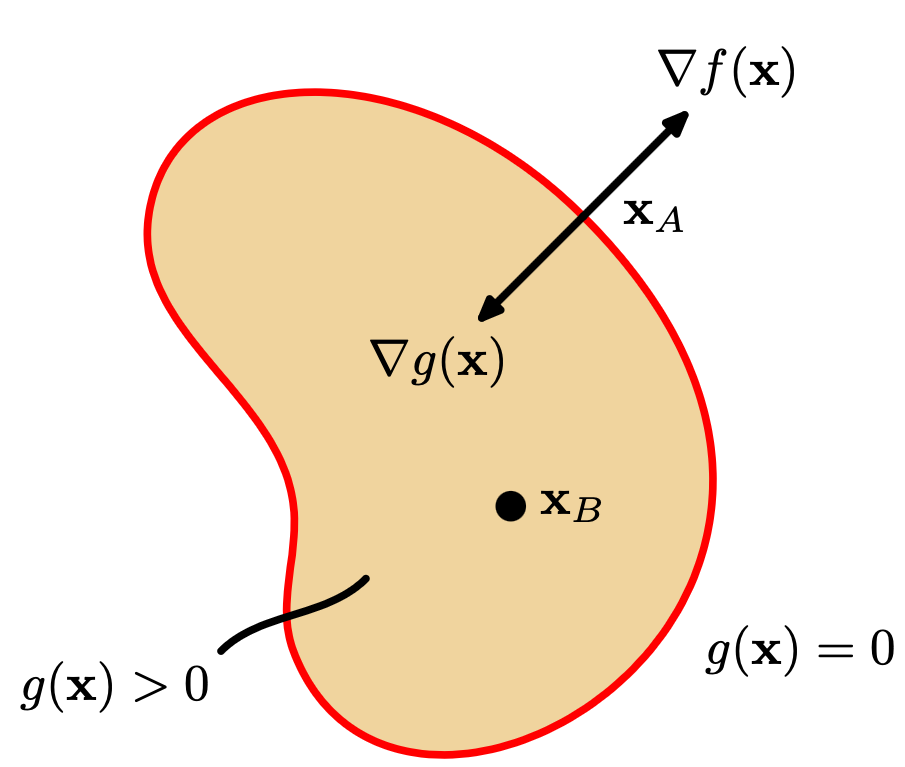
\includegraphics[width=5cm]{chapter005/figures/fig004}
    \caption{Lagrange Multipliers subject to $g(x) \geq 0$}
\end{figure}

Any support vector $x_n$ satisfies $t_ny(x_n)=1$, gives

\begin{equation}
    t_n (\sum_{m \in S} a_m t_m k(x_n, x_m) + b) = 1
\end{equation}

where $S$ denotes the set of indices of the support vectors.

\begin{equation}
    \begin{split}
    1 & = t_n (\sum_{m \in S} a_m t_m k(x_n, x_m) + b) \\
    & = t_n \sum_{m \in S} a_m t_m k(x_n, x_m) + t_nb \\
    \Leftrightarrow t_n & = t_n^2 \sum_{m \in S} a_m t_m k(x_n, x_m) + t_n^2b\\
    \Leftrightarrow t_n^2b & = t_n - t_n^2 \sum_{m \in S} a_m t_m k(x_n, x_m)\\
    \Leftrightarrow b & = t_n - \sum_{m \in S} a_m t_m k(x_n, x_m)\\
    \Leftrightarrow \sum_{n \in S} b & = \sum_{n \in S} (t_n - \sum_{m \in S} a_m t_m k(x_n, x_m))\\
    \Leftrightarrow N_S b & = \sum_{n \in S} (t_n - \sum_{m \in S} a_m t_m k(x_n, x_m))\\
    \Leftrightarrow b & = \frac{1}{N_S}\sum_{n \in S} (t_n - \sum_{m \in S} a_m t_m k(x_n, x_m))\\
    \end{split}
\end{equation}

where $N_S$ is the total number of support vectors.
Since $t_n=\pm 1$, $t_n^2=1$.

For later comparison with alternative models, we can express the maximum margin classifier in terms of the minimization of an error function, with a sample quadratic regularizer, in the form

\begin{equation}
    \label{form: svm error function}
    \sum_{n=1}^N E_\infty (y(x_n)t_n - 1) + \lambda ||w||^2
\end{equation}


Because the expected value of $y(x_n)t_n=1$, the \ref{form: svm error function} is minimum when $y(x_n)t_n=1$.

$E_\infty(z)$ is a function that is zero if $z \geq 0$ and $\infty$ otherwise and ensure that the constrain \ref{SVM: constraint} are satisfied.

 \section{Overlapping Class Distribution}
 
 We implicitly used an error function that gave infinite error if a data point was misclassified and zero error if it was classified correctly, and then optimized the model parameters to maximize the margin.
 
 We now modify this approach so that data points are allowed to be on the \textbf{wrong side} of the margin boundary, but with a penalty that increases with the distance from that boundary.
 
 To do this, we introduce \textbf{slack variables}, $\xi_n \geq 0$ where $n=1, ..., N$.
 
 These are defined by $\xi_n = 0$ for data points that are on or inside the correct margin boundary and $\xi_n = |t_n - y(x_n)|$ for other points. Thus a data point tht is on the decision boundary $y(x_n)=0$ will have $\xi_n=1$. $\xi_n > 1$ will be misclassified.
 
 The exact classification constraints are then replaced with
 \begin{equation}
    \label{SVM: slack variable constraint}
     t_ny(x_n) \geq 1 - \xi_n, n = 1,...,N
 \end{equation}
 in which the slack variables are constrained to satisfy $\xi \geq 0$. Data points for which $\xi \geq 0$ are correctly classified ($t_n = y(x_n)$). Points for which $0 < \xi \leq 1$ lie inside the margin, but on the correct side of the decision boundary. Those data points for which $\xi > 1$ lie on the wrong side of the decision boundary and are misclassified.
 
 
 \begin{figure}
    \centering
    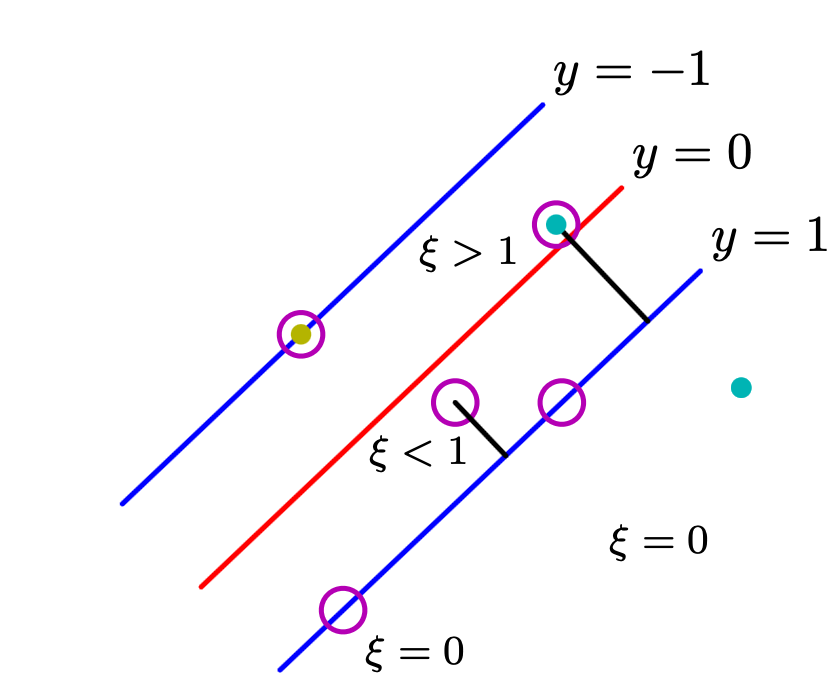
\includegraphics[width=5cm]{chapter005/figures/fig005}
    \caption{Illustration of the $\xi$ variable}
\end{figure}

This is sometimes described as relaxing the hard margin constraint to give a \textbf{soft margin} and allows some the training set data points to be misclassified.

Note that while slack variables allow for overlapping class distributions, this framework is still sensitive to outliers because the penalty for misclassification increases linearly with $\xi$.

Our goal is now to maximize the margin while softly penalizing points that lie on the wrong side of the margin boundary. We therefore minimize

\begin{equation}
    \label{SVM: C loss function}
    C \sum_{n=1}^N \xi_n + \frac{1}{2} ||w||^2
\end{equation}

where the parameter $C > 0$ controls the trade-off between the slack variable penalty and the margin. Because any point that is misclassified has $\xi > 1$, it follows that $\sum_n \xi_n$ is an upper bound on the number of misclassified points. The parameter $C$ is therefore analogous to a regularization coefficient because it controls the trade-off between minimizing training errors and controlling model complexity.

In the limit $C \rightarrow \infty$, we will recover the earlier support vector machine for separable data.

We now wish to minimize \ref{SVM: C loss function} subject to the constraints \ref{SVM: slack variable constraint} together with $\xi_n \geq 0$

The corresponding Lagrangian is given by

\begin{equation}
    \label{form: SVM Lagrangian}
    L(w, b, \xi, a, \mu) = \frac{1}{2} ||w||^2 + c\sum_{n=1}^N \xi_n - \sum_{n=1}^Na_n\{t_ny(x_n) - 1 + \xi_n\} - \sum_{n=1}^N \mu_n \xi_n
\end{equation}

Note that the constrain \ref{SVM: slack variable constraint} $\Leftrightarrow t_ny(x_n) - 1 + \xi_n \geq 0$
 
Where $\{a_n \geq 0\}$ and $\{\mu_n \geq 0 \}$ are Lagrange multipliers. The corresponding set of KKT conditions are given by


\begin{equation}
    \label{SVM: Lagrangian Soft-margin constraints}
  \left\{
    \begin{aligned}
      & a_n \geq 0\\
      & t_n y(x_n) - 1 + \xi_n \geq 0\\
      & a_n \{t_n y (x_n) - 1 + \xi_n \} = 0\\
      & \mu_n \geq 0\\
      & \xi_n \geq 0\\
      & \mu_n \xi_n = 0
    \end{aligned}
  \right.
\end{equation}

where $n=1,...,N$.

We know optimize out $w$, $b$ and $\{\xi_n\}$, then

\begin{equation}
    \frac{\partial L}{\partial w} = 0 \Leftrightarrow \frac{ \partial [\frac{1}{2} ||w||^2 - \sum_{n=1}^N a_n t_n w^T \phi(x_n) + \sum_{n=1}^N a_n t_n b - \sum_{n=1}^Na_n + \sum_{n=1}^Na_n \xi_n ]}{\partial w}= 0
\end{equation}

then,

\begin{equation}
    w - \sum_{n=1}^N a_n t_n \phi(x_n) = 0 \Leftrightarrow w = \sum_{n=1}^N a_n t_n \phi(x_n)
\end{equation}

In the similarity, we have

\begin{equation}
    \label{SVM: solution of Lagrange soft-margin}
  \left\{
    \begin{aligned}
      & \frac{\partial L}{\partial w} = 0 \Rightarrow \sum_{n=1}^N a_n t_n = 0\\
      & \frac{\partial L}{\partial \xi_n} = 0 \Leftrightarrow \sum_{n=1}^NC - \sum_{n=1}^Na_n - \sum_{n=1}^N \mu_n = 0 \Leftrightarrow  \sum_{n=1}^N(C - a_n - \mu_n) = 0 \Leftrightarrow a_n = C- \mu_n
    \end{aligned}
  \right.
\end{equation}

Then,

from \ref{form: SVM Lagrangian}, we have

\begin{equation}
    \label{SVM: Lagrange loss}
    L(a) = \sum_{n=1}^N a_n - \frac{1}{2}\sum_{n=1}^N\sum_{m=1}^N a_n a_m t_n t_m k(x_n, x_m)  
\end{equation}


which is identical to the separable case, except that the constraints are somewhat different. To see what these constraints are, we note that $a_n \geq 0$ is required because these are Lagrange multipliers.

Together with $u_n \geq 0$ implies $a_n \leq C$. We therefore have to maximize \ref{SVM:  Lagrange loss} with respect to the dual variables $\{a_n\}$ subject to

\begin{equation}
  \left\{
    \begin{aligned}
      & 0 \leq a_n \leq C\\
      & \sum_{n=1}^N a_n t_n = 0
    \end{aligned}
  \right.
\end{equation}

for $n=1, ..., N$.

\begin{enumerate}
    \item if $a_n = 0$, they do not contribute to the predictive model.
    \item if $a_n > 0$, from \ref{SVM: Lagrangian Soft-margin constraints}, we have $a_n(t_ny(x_n) -1 + \xi_n) = 0 \Leftrightarrow t_ny(x_n) -1 + \xi_n = 0$. Then, $t_ny(x_n) = 1 - \xi_n$.
    \item if $a_n < C$, then from \ref{SVM: solution of Lagrange soft-margin}, we have $a_n = C - \mu_n \Leftrightarrow \mu_n = C - a_n \Leftrightarrow \mu_n > 0$. From \ref{SVM: Lagrangian Soft-margin constraints}, we have $\mu_n \xi_n = 0$, thus $\xi_n = 0$. In other words, data points lie on the margin.
    \item if $a_n = C$, then $\mu_n = 0$. At this moment, we have 2 cases. If $\xi_n = 0$, then the points lie inside the margin. The last case is $\xi_n \neq 0$, it leads to 2 sub-cases. If $\xi_n \leq 1$, the points is correctly classified. Otherwise, they are misclassified.
\end{enumerate}




\appendix
\chapter{Vector}

\section{Representation and Position Vectors}

\begin{figure}[h]
    \centering
    \cite{calculus}
    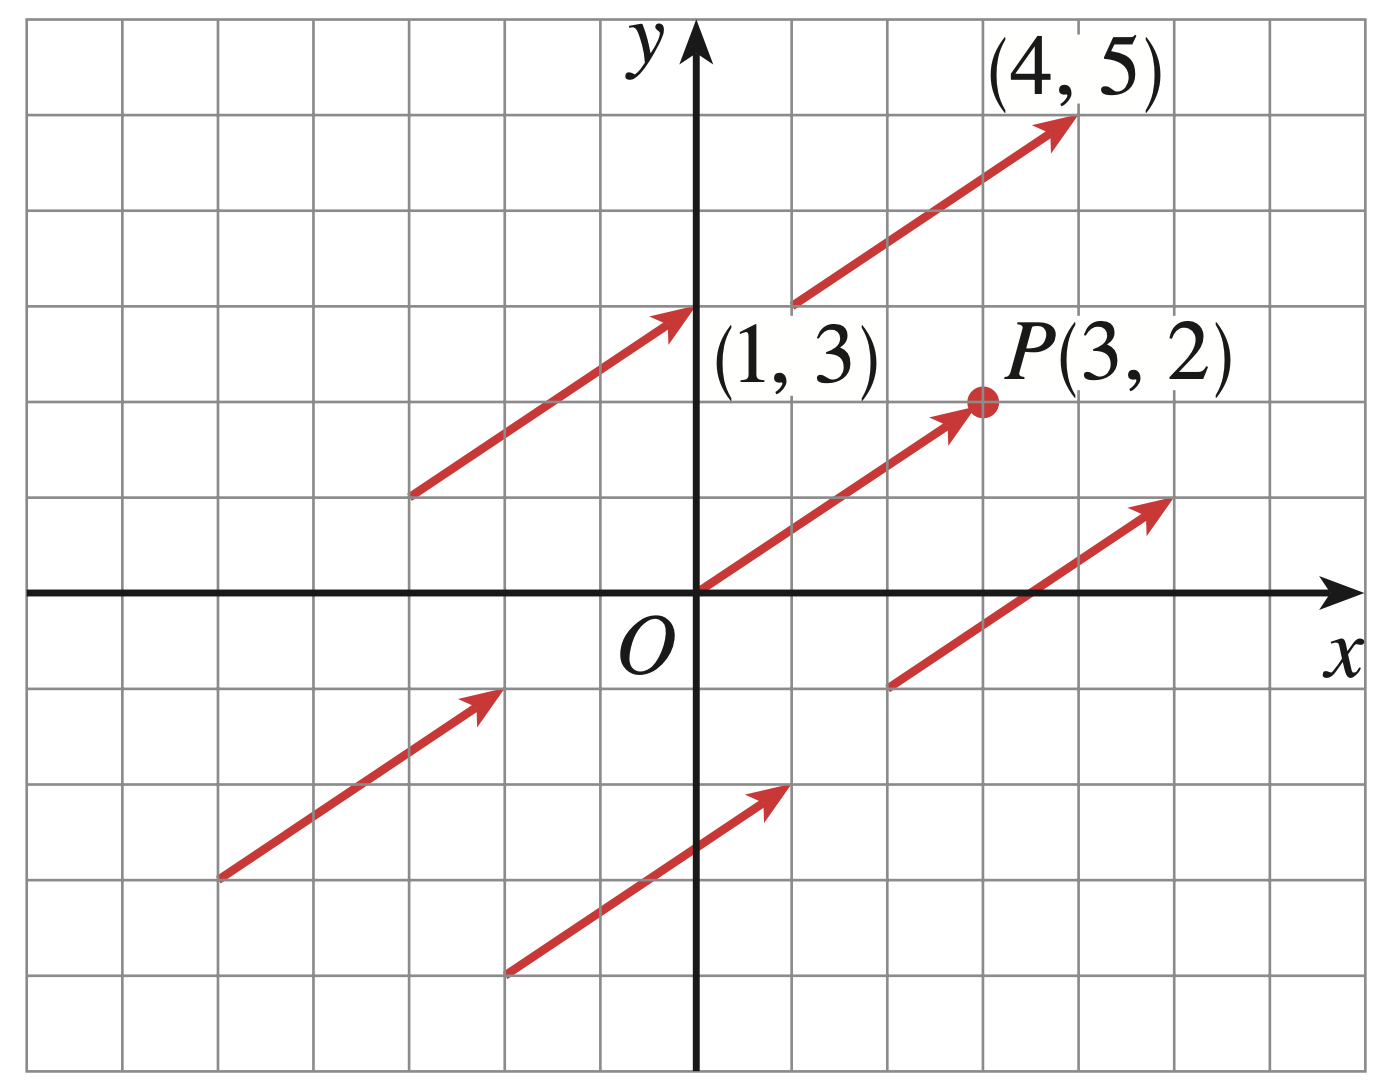
\includegraphics[scale=0.4]{appendices/figures/figure001}
    \caption{Basic Vectors}
    \label{Basic Vectors}
\end{figure}

All of the vectors shown in the above figure are equivalent to the vector $\vec{OP}=<3, 2>$ whose terminal point is $P(3, 2)$. What they have in common is that the
terminal point is reached from the initial point by a displacement of three units to the right and two upward. We can think of all these geometric vectors as \textbf{representations} of the algebraic vector $\vec{a}=<3, 2>$. The particular representation $\vec{OP}$ from the origin to the point $P(3, 2)$ is called the \textbf{position vector} of the point $P$.

\begin{definition}
Given the points $A(x_1, y_1, z_1)$ and $B(x_2, y_2, z_2)$, the vector $\vec{a}$ with representation $\vec{AB}$ is
    \begin{equation}
        \vec{a} = <x_2 - x_1, y_2 - y_1, z_2 - z_1>
    \end{equation}
\end{definition}

\begin{figure}[h]
    \centering
    \cite{calculus}
    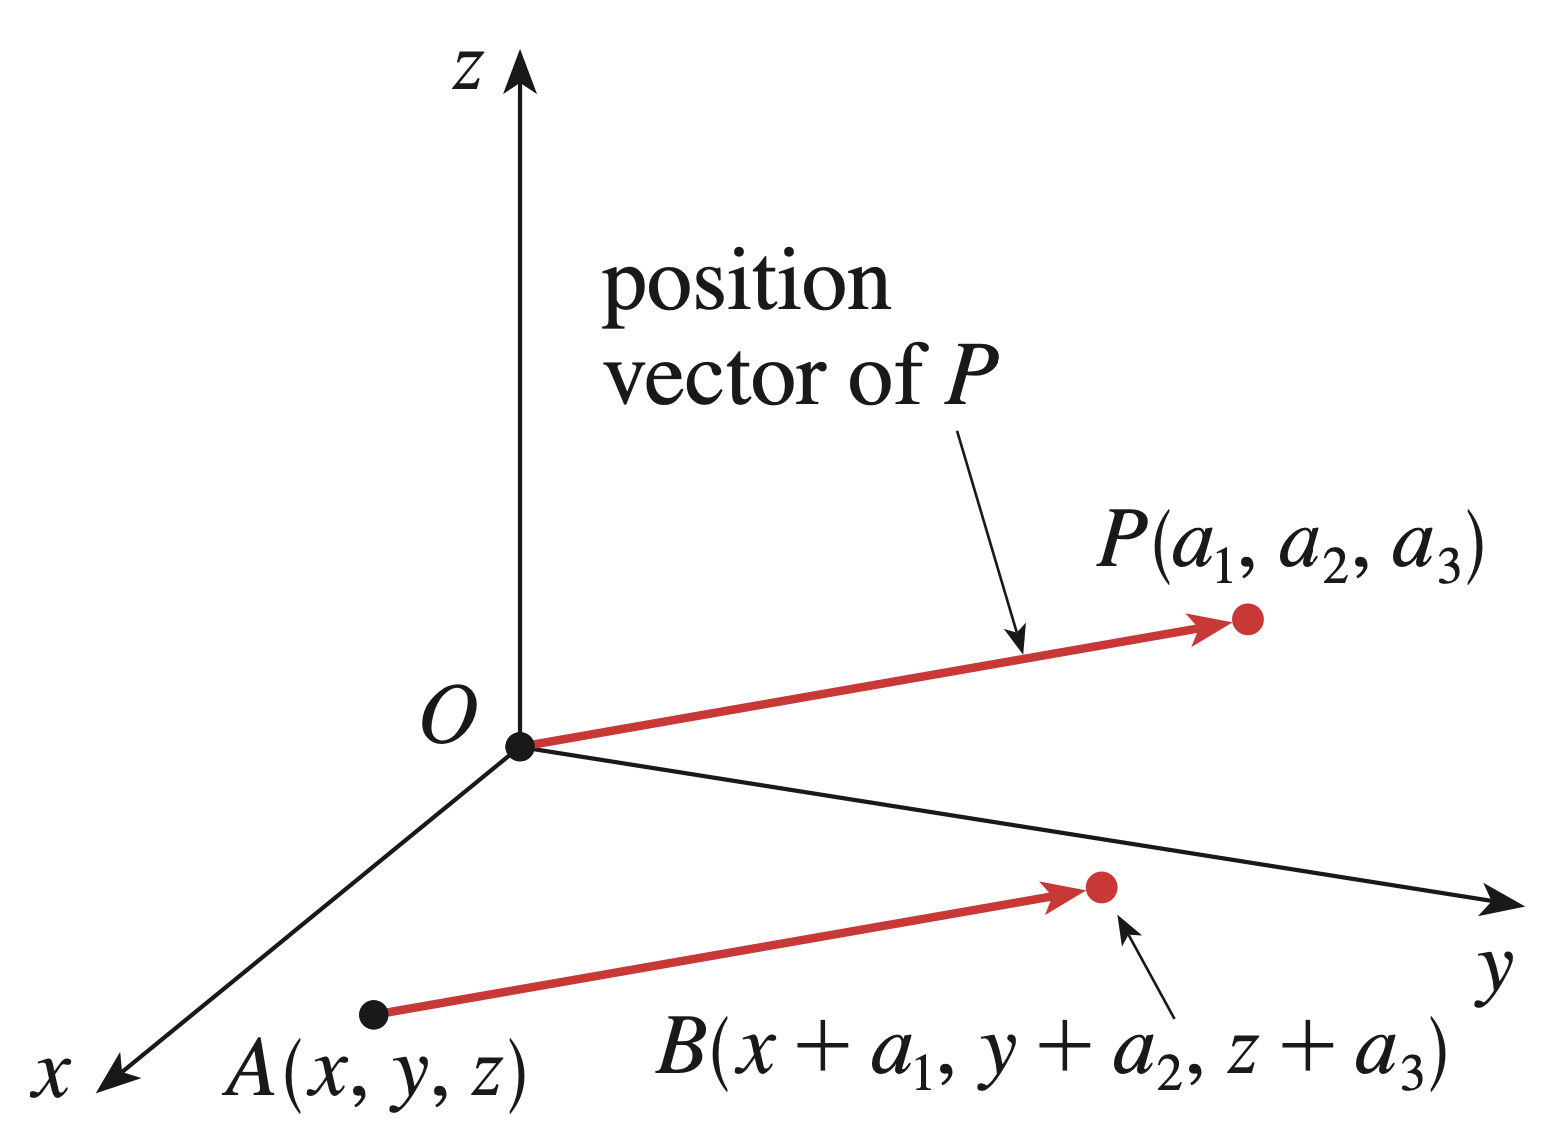
\includegraphics[scale=0.45]{appendices/figures/figure002}
    \caption{Position Vectors}
    \label{Position Vectors}
\end{figure}

\section{Projections}

\begin{figure}[h]
    \centering
    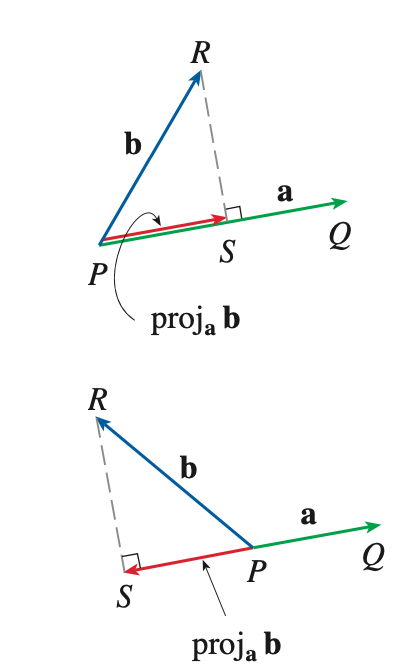
\includegraphics[scale=0.45]{appendices/figures/fig006}
    \caption{Vector projection}
    \label{Vector projection}
\end{figure}

In the figure \ref{Vector projection}, if $S$ is the foot of the perpendicular from $R$ to $\vec{PQ}$, then the vector with representation $\vec{PS}$ is called the \textbf{vector projection} of \textbf{b} onto \textbf{a} and is denoted by $proj_ab$.

The scalar projection of \textbf{b} onto \textbf{a} which is also called \textbf{component of b along a} is denoted by $comp_ab$.

\begin{equation}
    comp_ab = \frac{a \cdot b}{|a|}
\end{equation}

\begin{equation}
    proj_ab = (\frac{a \cdot b}{|a|}) \frac{a}{|a|} = \frac{a \cdot b}{|a|^2}a
\end{equation}

Note that $\frac{a}{|a|}$ is a unit vector. $\frac{a \cdot b}{|a|}$ and $\frac{1}{|a|}$ are numbers and $a$ is a vector.
\chapter{Equations of Lines and Planes}

\section{Lines}

A line $L$ in three-dimensional space is determined when we know a point $P_0(x_0, y_0, z_0)$ on $L$ and a direction for $L$, which is conveniently described by a vector $\vec{v}$ parallel to the line.

Let $P(x, y, z)$ be an arbitrary point on $L$ and let $\vec{r_0}$ and $\vec{r}$ be the position vectors of $P_0$ and $P$. At this moment, $\vec{r_0}$ and $\vec{r}$ have representations $\vec{OP_0}$ and $\vec{OP}$, respectively. Thus, $\vec{r} = \vec{r_0} + \vec{a}$

\begin{figure}
    \centering
    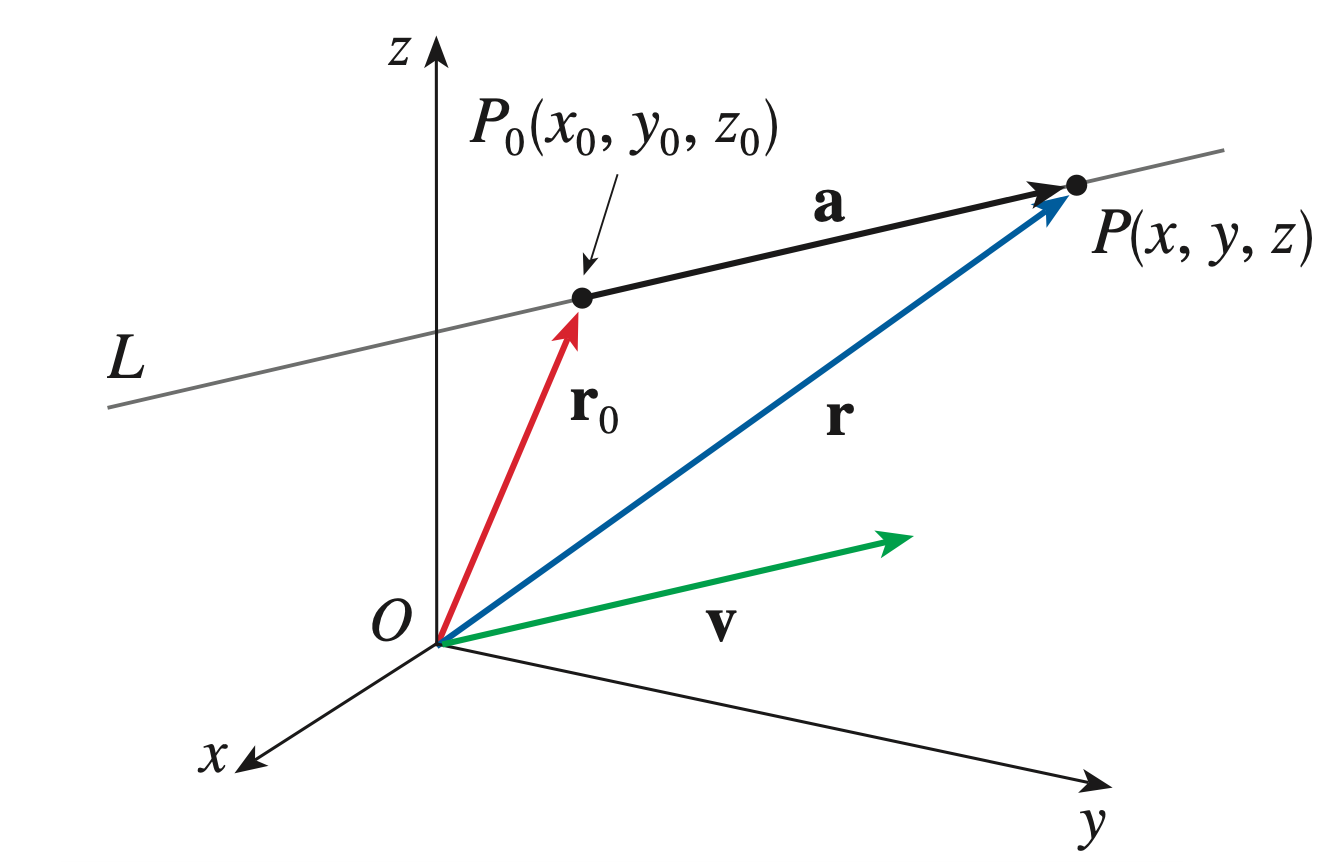
\includegraphics[width=8cm]{appendices/figures/fig003.png}
    \caption{Line representation}
\end{figure}

In the following figure, we have $\vec{v}$ is paralleled to $\vec{a}$, then $\vec{a} = t\vec{v}$. Thus, $\vec{r} = \vec{r_0} + t\vec{v}$ which is a \textbf{vector equation} of L. Each value of the parameter t gives the position vector $\vec{r}$ of a point on $L$.

\begin{figure}
    \centering
    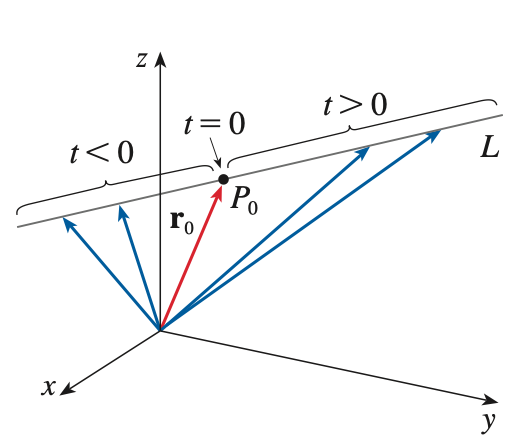
\includegraphics[width=8cm]{appendices/figures/fig004.png}
    \caption{Line representation}
\end{figure}

Given $v = <a, b, c>$, $r=<x, y, z>$ and $r_0=<x_0, y_0, z_0>$, then

\begin{equation}
    <x, y, z> = <x_0 + ta, y_0 + tb, z_0 + tc>
\end{equation}

Two vectors are equal if and only if corresponding components are equal. Therefore, we have three scalar equations:

\begin{equation}
    \label{parametric equation}
  \left\{
    \begin{aligned}
      & x = x_0 + ta\\
      & y = y_0 + tb\\
      & z = z_0 + tc
    \end{aligned}
  \right.
\end{equation}

where $t \in \mathbb{R}$.

These equations are called \textbf{parametric equations} of the line L through the point $P_0(x_0, y_0, z_0)$ and parallel to the vector $\vec{v} = <a, b, c>$. Each value of $t$ gives a point $(x, y, z)$ on $L$.

From the \ref{parametric equation} we have,

\begin{equation}
    \label{symmetric equation}
    \frac{x - x_0}{a} = \frac{y - y_0}{b} = \frac{z - z_0}{c}
\end{equation}

If the line pass through one more point $r_1$, then $\vec{v} = r_1 - r_0$ and

\begin{equation}
    r = r_0 + t(r_1 - r_0) = (1 - t)r_0 + tr_1
\end{equation}


\section{Planes}

A single vector parallel to the plane is not enough to convey the "direction" of the plane, but a vector perpendicular to the planes does completely specify its direction. Thus a plane is space is determined by a point $P_0(x_0, y_0, z_0)$ in the plane and a vector $\vec{n}$ that is orthogonal to the plane. This orthogonal vector $\vec{n}$ is called a \textbf{normal vector}.

Let $P(x, y, z)$ be an arbitrary point the plane, and let $\vec{r_0}$ and $\vec{r}$ be the position vectors of $P_0$ and $P$. Then the vector $\vec{r} - \vec{r_0}$ is represented by $\vec{P_0P}$

The normal vector $\vec{n}$ is orthogonal to every vector in the given plane. In particular, $\vec{n}$ is orthogonal to $\vec{r} - \vec{r_0}$ and so we have

\begin{figure}
    \centering
    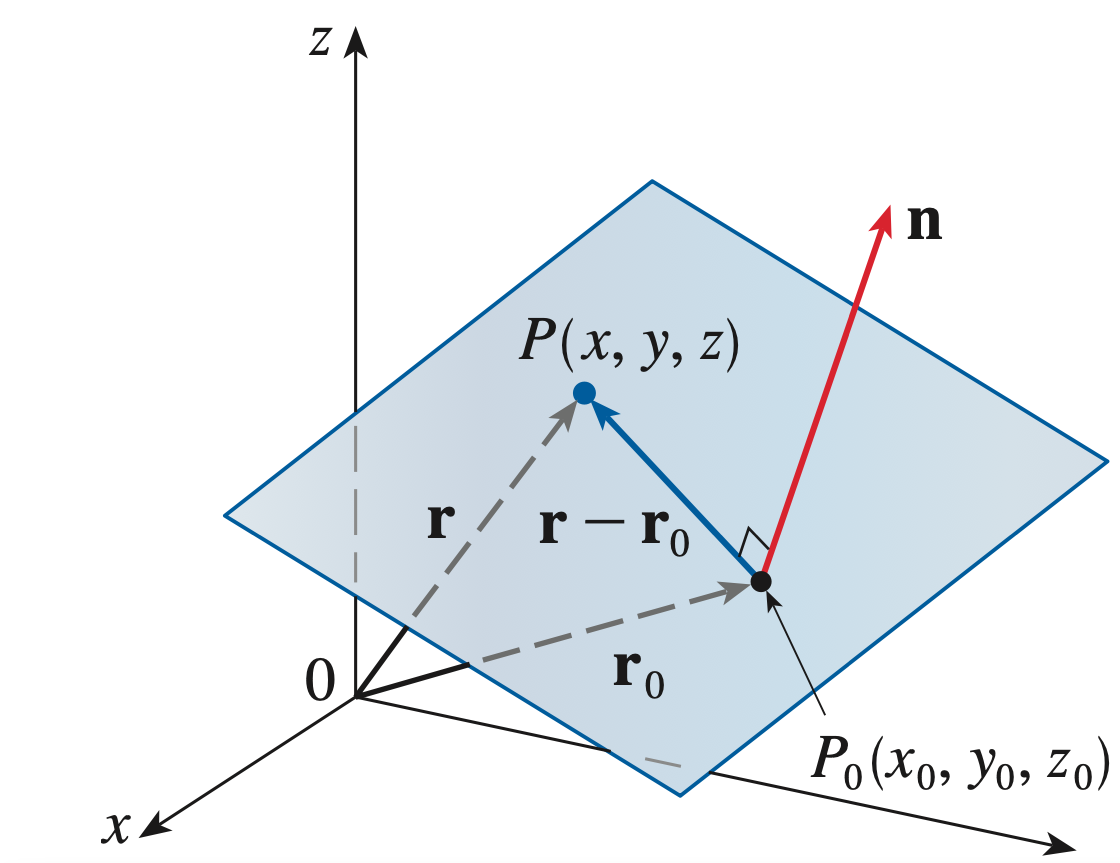
\includegraphics[width=8cm]{appendices/figures/fig005}
    \caption{Line representation}
\end{figure}

\begin{equation}
    \label{Vector equation of a plane}
    n \cdot (\vec{r} - \vec{r_0}) = 0 \Leftrightarrow n \cdot r = n \cdot r_0
\end{equation}

\ref{Vector equation of a plane} is called \textbf{Vector equation of a plane}.

Given $n = <a, b, c>, r = <x, y, z>$ and $r_0 = <x_0, y_0, z_0>$, then

\begin{equation}
    <a, b, c> \cdot <x - x_0, y - y_0, z - z_0> = 0
\end{equation}

In other words,

\begin{equation}
    \label{Linear equation of the plane}
    \begin{split}
        a(x - x_0) + b(y - y_0) + c(z - z_0) & = 0\\
        \Leftrightarrow ax - ax_0 + by - by_0 + cz - cz_0 & = 0\\
        \Leftrightarrow ax + by + cz - ax_0 - by_0 - cz_0 & = 0\\
        \Leftrightarrow ax + by + cz + d = 0
    \end{split}
\end{equation}

where $d = -(ax_0 + by_0 + cz_0)$ 

\ref{Linear equation of the plane} is called a \textbf{linear equation}.

In machine learning, we usually,

\begin{align}
    w &= \begin{bmatrix}
           a \\
           b \\
           c
         \end{bmatrix}
\end{align}

and

\begin{align}
    x &= \begin{bmatrix}
           x_1 \\
           x_2 \\
           x_3
         \end{bmatrix}
  \end{align}

where $x$ is a data point and $x_1, x_2$ and $x_3$ is its vector components. Then, \ref{Linear equation of the plane} is represented as

\begin{equation}
    w^Tx + d = 0    
\end{equation}

Thus, $w$ is \textbf{normal vector} of the plane.

\section{Distance}

In order to find a formula for the distance $D$ from a point $P_1(x_1, y_1, z_1)$ to the plane $ax + by + cz + d = 0$, we let $P_0(x_0, y_0, z_0)$ be any point in the given plane and $\vec{b}$ be the vector corresponding to $\vec{P_0P_1}$. Then,

\begin{equation}
    b = <x_1 - x_0, y_1 - y_0, z_1 - z_0>
\end{equation}

the distance $D$ from $P_1$ to the plane is equal to the absolute value of the scalar projection of $\vec{b}$ onto the normal vector $\vec{n} = <a, b, c>$. Thus,

\begin{equation}
    \begin{split}
        D & = ||comp_n\vec{b}|\\
          & = \frac{|n \cdot b|}{|n|}\\
          & = \frac{|a(x_1 - x_0) + b(y_1 - y_0) + c(z_1 - z_0)|}{\sqrt{a^2 + b^2 + c^2}}\\
          & = \frac{|ax_1 + by_1 + cz_1 + d|}{\sqrt{a^2 + b^2 + c^2}}
    \end{split}
\end{equation}


\chapter{Matrices}

\section{Symmetric Matrices}

Given a matrix $A_{3x3}$ defined as

$$
A = 
\begin{bmatrix}
a_{11} & a_{12} & a_{13}\\
a_{21} & a_{22} & a_{23}\\
a_{31} & a_{32} & a_{33}
\end{bmatrix}
$$

thus,

$$
A^T = 
\begin{bmatrix}
a_{11} & a_{21} & a_{31}\\
a_{12} & a_{22} & a_{32}\\
a_{13} & a_{23} & a_{33}
\end{bmatrix}
$$

\begin{equation}
    AA^T = 
    \begin{bmatrix}
        (a_{11}a_{11} + a_{12}a_{12} + a_{13}a_{13}) & (a_{11}a_{21} + a_{12}a_{22} + a_{13}a_{23}) & (a_{11}a_{31} + a_{12}a_{32} + a_{13}a_{33})\\
        (a_{21}a_{11} + a_{22}a_{12} + a_{23}a_{13}) & (a_{21}a_{21} + a_{22}a_{22} + a_{23}a_{23}) & (a_{21}a_{31} + a_{22}a_{32} + a_{23}a_{33})\\
        (a_{31}a_{11} + a_{32}a_{12} + a_{33}a_{13}) & (a_{31}a_{21} + a_{32}a_{22} + a_{33}a_{23}) & (a_{31}a_{31} + a_{32}a_{32} + a_{33}a_{33})
    \end{bmatrix}    
\end{equation}

let

$$
K = (a_{11}a_{11} + a_{12}a_{12} + a_{13}a_{13})
$$

$$
L = (a_{11}a_{21} + a_{12}a_{22} + a_{13}a_{23})
$$

$$
H = (a_{11}a_{31} + a_{12}a_{32} + a_{13}a_{33})
$$

$$
M = (a_{21}a_{21} + a_{22}a_{22} + a_{23}a_{23})
$$

$$
N = (a_{21}a_{31} + a_{22}a_{32} + a_{23}a_{33})
$$

$$
G = (a_{31}a_{31} + a_{32}a_{32} + a_{33}a_{33})
$$

then,

\begin{equation}
    AA^T = 
    \begin{bmatrix}
        K & L & H\\
        L & M & N\\
        H & N & G
    \end{bmatrix}    
\end{equation}

and

$$
(AA^T)^T = 
\begin{bmatrix}
    K & L & H\\
    L & M & N\\
    H & N & G
\end{bmatrix}
$$

therefore,

\begin{equation}
    AA^T = (AA^T)^T
\end{equation}

In conclusion, $AA^T$ is a symmetric matrix.

\section{Derivatives}
Given

$$
w = 
\begin{bmatrix}
    w_1\\
    w_2\\
    w_3
\end{bmatrix}
\ \ \ \ A =
\begin{bmatrix}
    a_{11} & a_{12} & a_{13}\\
    a_{21} & a_{22} & a_{23}\\
    a_{31} & a_{32} & a_{33}
\end{bmatrix}
$$

thus,

$$
w^TAw =
[w_1\ w_2\ w_3]
\begin{bmatrix}
    a_{11} & a_{12} & a_{13}\\
    a_{21} & a_{22} & a_{23}\\
    a_{31} & a_{32} & a_{33}
\end{bmatrix}
\begin{bmatrix}
    w_1\\
    w_2\\
    w_3
\end{bmatrix}
$$

$$
w^TAw =
\begin{bmatrix}
    (w_1a_{11} + w_2a_{21} + w_3a_{31}) & (w_1a_{12} + w_2a_{22} + w_3a_{32}) & (w_1a_{13} + w_2a_{23} + w_3a_{33})\\
\end{bmatrix}
\begin{bmatrix}
    w_1\\
    w_2\\
    w_3
\end{bmatrix}
$$

$$
\Leftrightarrow w^TAw =
    (w_1w_1a_{11} + w_1w_2a_{21} + w_1w_3a_{31}) + (w_2w_1a_{12} + w_2w_2a_{22} + w_2w_3a_{32}) + (w_3w_1a_{13} + w_3w_2a_{23} + w_3w_3a_{33})\\
$$

if $A$ is a symmetric matrix, then $a_{21} = a_{12}$, $a_{13} = a_{31}$, $a_{32} = a_{23}$

then,
$$
w^TAw =
    (w_1w_1a_{11} + w_1w_2a_{12} + w_1w_3a_{13}) + (w_2w_1a_{12} + w_2w_2a_{22} + w_2w_3a_{23}) + (w_3w_1a_{13} + w_3w_2a_{23} + w_3w_3a_{33})\\
$$

$$
w^TAw =
    (w_1w_1a_{11} + 2w_1w_2a_{12} + 2w_1w_3a_{13}) + (w_2w_2a_{22} + 2w_2w_3a_{23} +w_3w_3a_{33})\\
$$

$$
\frac{\partial (w^TAw)}{\partial w_1} = \frac{2w_1a_{11} + 2w_2a_{12} + 2w_3a_{13}}{\partial w_1}
$$

$$
\frac{\partial (w^TAw)}{\partial w_2} = \frac{2w_1a_{12} + 2w_2a_{22} + 2w_3a_{23}}{\partial w_2}
$$

$$
\frac{\partial (w^TAw)}{\partial w_3} = \frac{2w_1a_{31} + 2w_2a_{23} + 2w_3a_{33}}{\partial w_3}
$$
in other words,

\begin{equation}
    \frac{\partial w^TAw}{\partial w} = 
    \begin{bmatrix}
        2w_1a_{11} + 2w_2a_{12} + 2w_3a_{13}\\
        2w_1a_{12} + 2w_2a_{22} + 2w_3a_{23}\\
        2w_1a_{31} + 2w_2a_{23} + 2w_3a_{33}
    \end{bmatrix}
\end{equation}


since,

$$
Aw = 
\begin{bmatrix}
    a_{11}w_1 + a_{12}w_2 + a_{13}w_3\\
    a_{21}w_1 + a_{22}w_2 + a_{23}w_3\\
    a_{31}w_1 + a_{32}w_2 + a_{33}w_3
\end{bmatrix}
$$

thus

\begin{equation}
    \frac{\partial w^TAw}{\partial w} = 2Aw
\end{equation}






\chapter{Integrals}

\section{Change of Variables in Double Integrals}

The new variable $r$ and $\theta$ are related to the old variables $x$ and $y$ by the equations

\begin{align}
    x = r\cos \theta && y = r\sin \theta
\end{align}

We consider a change of variables that is given by a transformation $T$ from the $uv$-plane to the $xy$-plane

\begin{equation}
    T(u, v) = (x, y)
\end{equation}

where $x$ and $y$ are related to $u$ and $v$ by the equations

\begin{align}
    x = g(u, v) && y = h(u, v)
\end{align}

we usually assume that $T$ is a $C^1$ transformation, which means that $g$ and $h$ have continuous first-order partial derivatives.

A transformation $T$ is really just a function whose domain and range are both subsets of $\mathbb{R}^2$.

If $T(u_1, v_1)=(x_1, y_1)$, then the point $(x_1, y_1)$ is called the \textbf{image} of the point $(u_1, v_1)$.

If no two points have the same image, $T$ is called \textbf{one-to-one}.

\begin{figure}
    \centering
    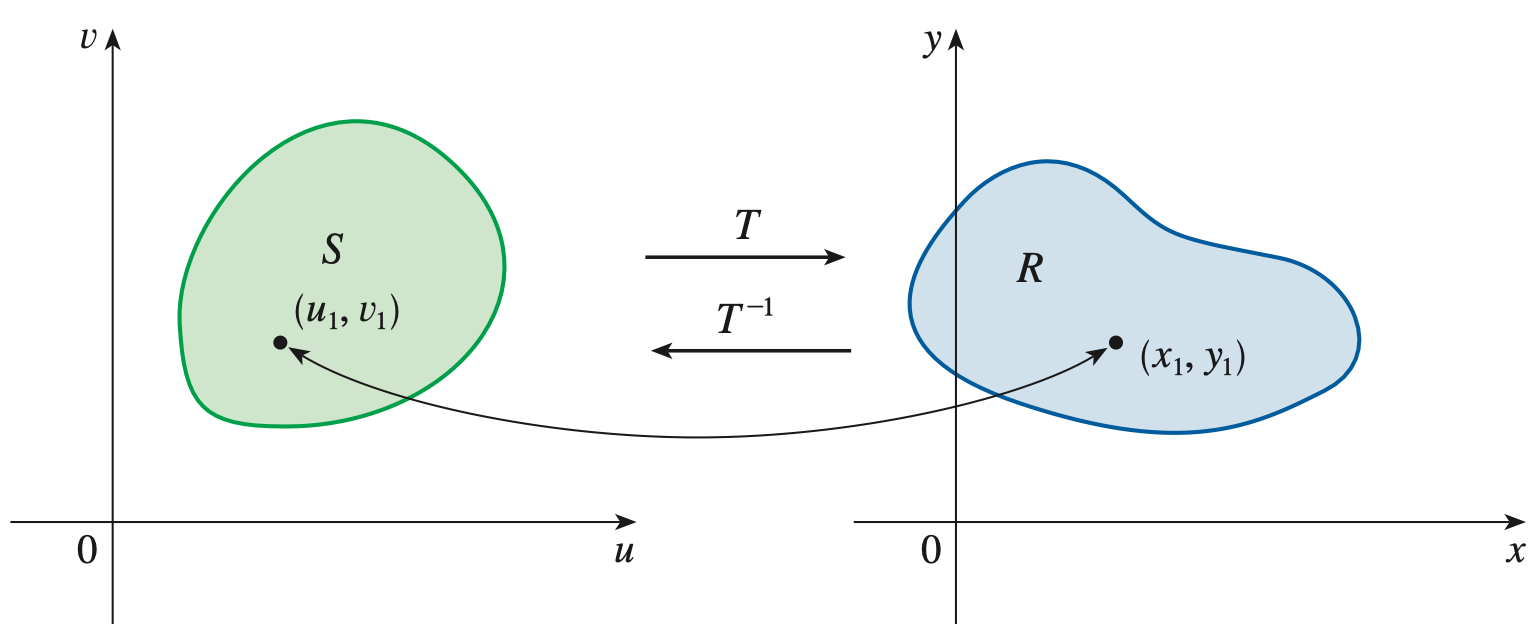
\includegraphics[scale=0.3]{appendices/figures/fig008.png}
    \caption{One-to-one Transformation}
\end{figure}

$T$ transforms $S$ into a region $R$ in the $xy$-plane called the \textbf{image of S}, consisting of the images of all points in $S$.

If $T$ is a one-to-one transformation, then it has an \textbf{inverse transformation} $T^{-1}$ from the $xy$-plane to the $uv$-plane.

\begin{figure}
    \centering
    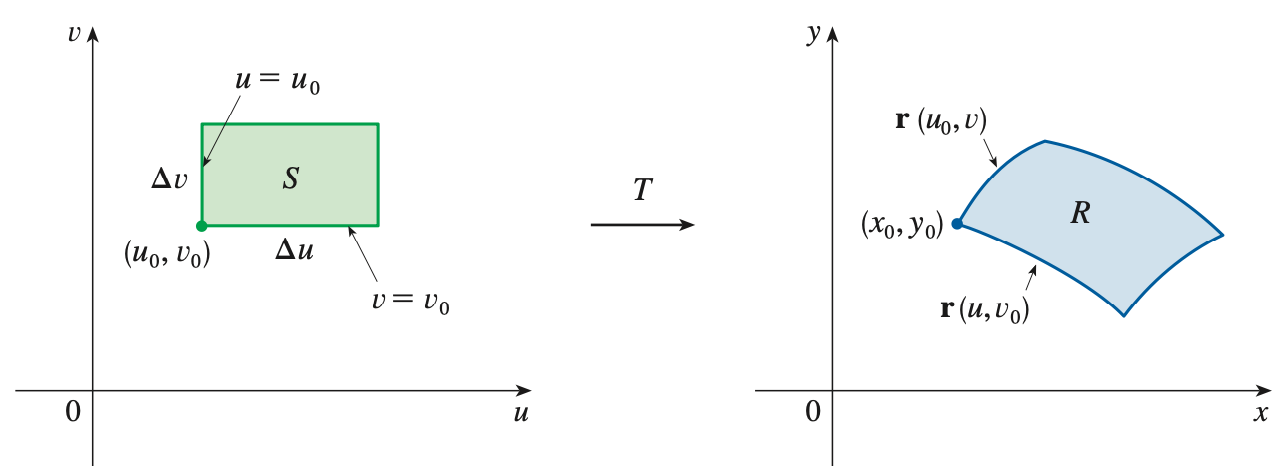
\includegraphics[scale=0.3]{appendices/figures/fig009.png}
    \caption{A change of variables affects a double integral}
\end{figure}

We start with a small rectangle $S$ in the $uv$-plane whose lower left corner is the point $(u_0, v_0)$ and whose dimensions are $\Delta u$ and $\Delta v$.

The image of $S$ is a region $R$ in the $xy$-plane, one of whose boundary points $(x_0, y_0)$ = $T(u_0, v_0)$. The vector $r(u, v)$ is defined as

\begin{equation}
    r(u, v) = g(u, v) \mathbf(i) + h(u, v) \mathbf(j)
\end{equation}

The vector $r(u, v)$ is the position vector of the image of the point $(u, v)$ .

The equation of the lower side of $S$ is $v = v_0$, whose image curve is given by the vector function $r(u, v_0)$. The tangent vector at $(x_0, y_0)$ to this image curve is

\begin{equation}
    r_u = g_u(u_0, v_0)\mathbf{i} + h_u(u_0, v_0)\mathbf{j} = \frac{\partial x}{\partial u}\mathbf{i} + \frac{\partial y}{\partial u}\mathbf{j}
\end{equation}

\begin{figure}
    \centering
    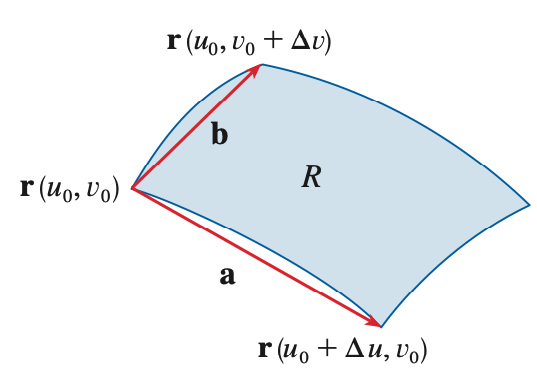
\includegraphics[scale=0.3]{appendices/figures/fig010.png}
    \caption{A change of variables affects a double integral}
\end{figure}

Similarity, the tangent vector at $(x_0, y_0)$ to the image curve of the left side of $S$ is

\begin{equation}
    r_v = g_v(u_0, v_0)\mathbf{i} + h_v(u_0, v_0)\mathbf{j} = \frac{\partial x}{\partial v}\mathbf{i} + \frac{\partial y}{\partial v}\mathbf{j}
\end{equation}

We can approximate the image region $R=T(S)$ by a parallelogram determined by the secant vectors

\begin{align}
    a = r(u_0 + \Delta u, v_0) - r(u_0, v_0) && b = r(u_0, v_0 + \Delta v) - r(u_0, v_0)
\end{align}

but 

\begin{equation}
    r_u = \lim_{\Delta u \rightarrow 0} \frac{r(u_0 + \Delta u, v_0) - r(u_0, v_0)}{\Delta u}
\end{equation}

and so

\begin{equation}
    r(u_0 + \Delta u, v_0) - r(u_0, v_0) \approx \Delta u r_u
\end{equation}

similarity

\begin{equation}
    r(u_0, v_0 + \Delta v) - r(u_0, v_0) \approx \Delta v r_v
\end{equation}

This means that we can approximate $R$ by a parallelogram determined by the vectors $\Delta u r_u$ and $\Delta v r_v$

\begin{figure}
    \centering
    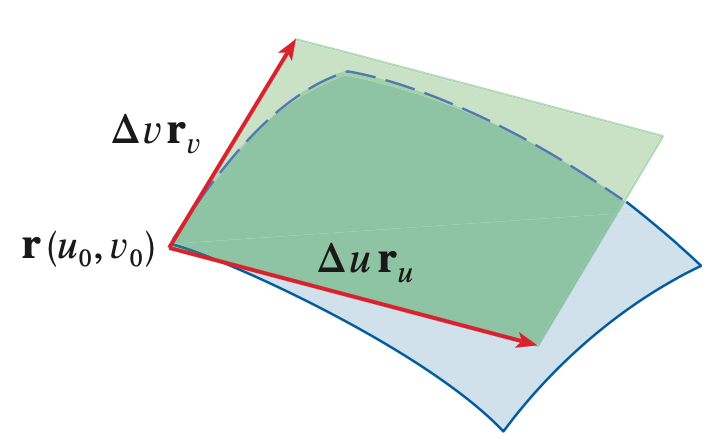
\includegraphics[scale=0.3]{appendices/figures/fig011.png}
    \caption{A change of variables affects a double integral}
\end{figure}

Therefore we can approximate the area of $R$ by the area of this parallelogram, which is

\begin{equation}
    |(\Delta u r_u) \times (\Delta v r_v)| = |r_u \times r_v| \Delta u \Delta v
\end{equation}

Computing the cross product, we obtain

\begin{align*}
    \vec{r_u} \times \vec{r_v} = 
    \begin{vmatrix}
        \mathbf{i} & \mathbf{j} & \mathbf{k}\\
        \frac{\partial x}{\partial u} & \frac{\partial y}{\partial u} & 0\\
        \frac{\partial x}{\partial v} & \frac{\partial y}{\partial v} & 0
    \end{vmatrix}
     = 
     \begin{vmatrix}
        \frac{\partial x}{\partial u} & \frac{\partial y}{\partial u}\\
        \frac{\partial x}{\partial v} & \frac{\partial y}{\partial v}
    \end{vmatrix}
    \mathbf{k} =
     \begin{vmatrix}
        \frac{\partial x}{\partial u} & \frac{\partial x}{\partial v}\\
        \frac{\partial y}{\partial u} & \frac{\partial y}{\partial v}
    \end{vmatrix}
    \mathbf{k}
\end{align*}

The determinant that arises in this calculation is called the \textbf{Jacobian}

\begin{definition}
    The Jacobian of transformation T given by $x=g(u, v)$ and $y=h(u, v)$ is
    
    \begin{align*}
    \frac{\partial(x, y)}{\partial (u, v)} = 
     \begin{vmatrix}
        \frac{\partial x}{\partial u} & \frac{\partial x}{\partial v}\\
        \frac{\partial y}{\partial u} & \frac{\partial y}{\partial v}
    \end{vmatrix}
    =
    \frac{\partial x}{\partial u} \frac{\partial y}{\partial v} - \frac{\partial x}{\partial v}\frac{\partial y}{\partial u}
    \end{align*}
\end{definition}

\begin{definition}
    Suppose that $T$ is a $C^1$ transformation whose Jacobian is nonzero and that $T$ maps a region $S$ in the $uv$-plane onto a region R in the $xy$-plane. Suppose that $f$ is continuous on $R$ and that $R$ and $S$ are type I and type II plane regions. Suppose also that $T$ is one-to-one, except perhaps on the boundary of $S$. Then
\end{definition}

\begin{align*}
    \iint_{R} f(x, y)dA = 
    \iint_{S}f(x(u, v), y(u, v))
    \begin{vmatrix}
        \frac{\partial(x, y)}{\partial (u, v)}
    \end{vmatrix}
  dudv
\end{align*}


\bibliographystyle{plain}
\bibliography{refs/refs}

\end{document}